%%% Hlavní soubor. Zde se definují základní parametry a odkazuje se na ostatní části. %%%

%% Verze pro jednostranný tisk:
% Okraje: levý 40mm, pravý 25mm, horní a dolní 25mm
% (ale pozor, LaTeX si sám přidává 1in)
\documentclass[12pt,a4paper]{report}
\setlength\textwidth{145mm}
\setlength\textheight{247mm}
\setlength\oddsidemargin{15mm}
\setlength\evensidemargin{15mm}
\setlength\topmargin{0mm}
\setlength\headsep{0mm}
\setlength\headheight{0mm}
% \openright zařídí, aby následující text začínal na pravé straně knihy
\let\openright=\clearpage

%% Pokud tiskneme oboustranně:
% \documentclass[12pt,a4paper,twoside,openright]{report}
% \setlength\textwidth{145mm}
% \setlength\textheight{247mm}
% \setlength\oddsidemargin{14.2mm}
% \setlength\evensidemargin{0mm}
% \setlength\topmargin{0mm}
% \setlength\headsep{0mm}
% \setlength\headheight{0mm}
% \let\openright=\cleardoublepage

%% Vytváříme PDF/A-2u
\usepackage[a-2u]{pdfx}

%% Přepneme na českou sazbu a fonty Latin Modern
\usepackage[czech]{babel}
\usepackage{lmodern}
\usepackage[T1]{fontenc}
\usepackage{textcomp}

%% Použité kódování znaků: obvykle latin2, cp1250 nebo utf8:
\usepackage[utf8]{inputenc}

%%% Další užitečné balíčky (jsou součástí běžných distribucí LaTeXu)
\usepackage{amsmath}        % rozšíření pro sazbu matematiky
\usepackage{amsfonts}       % matematické fonty
\usepackage{amsthm}         % sazba vět, definic apod.
\usepackage{bbding}         % balíček s nejrůznějšími symboly
			    % (čtverečky, hvězdičky, tužtičky, nůžtičky, ...)
\usepackage{bm}             % tučné symboly (příkaz \bm)
\usepackage{graphicx}       % vkládání obrázků
\usepackage{fancyvrb}       % vylepšené prostředí pro strojové písmo
\usepackage{indentfirst}    % zavede odsazení 1. odstavce kapitoly
\usepackage{natbib}         % zajištuje možnost odkazovat na literaturu
			    % stylem AUTOR (ROK), resp. AUTOR [ČÍSLO]
\usepackage[nottoc]{tocbibind} % zajistí přidání seznamu literatury,
                            % obrázků a tabulek do obsahu
\usepackage{icomma}         % inteligetní čárka v matematickém módu
\usepackage{dcolumn}        % lepší zarovnání sloupců v tabulkách
\usepackage{booktabs}       % lepší vodorovné linky v tabulkách
\usepackage{paralist}       % lepší enumerate a itemize
\usepackage{xcolor}         % barevná sazba

\usepackage{tikz}			% tikz

%%% Údaje o práci

% Název práce v jazyce práce (přesně podle zadání)
\def\NazevPrace{Interakce testovacích částic s impulzními gravitačními vlnami}

% Název práce v angličtině
\def\NazevPraceEN{Interaction of test particles with impulsive gravitational waves}

% Jméno autora
\def\AutorPrace{Daniel Rod}

% Rok odevzdání
\def\RokOdevzdani{2021}

% Název katedry nebo ústavu, kde byla práce oficiálně zadána
% (dle Organizační struktury MFF UK, případně plný název pracoviště mimo MFF)
\def\Katedra{Ústav teoretické fyziky}
\def\KatedraEN{Institute of Theorethical Physics}

% Jedná se o katedru (department) nebo o ústav (institute)?
\def\TypPracoviste{Ústav}
\def\TypPracovisteEN{Institute}

% Vedoucí práce: Jméno a příjmení s~tituly
\def\Vedouci{RNDr. Robert Švarc, Ph.D.}

% Pracoviště vedoucího (opět dle Organizační struktury MFF)
\def\KatedraVedouciho{Ústav teoretické fyziky}
\def\KatedraVedoucihoEN{Institute of Theorethical Physics}

% Studijní program a obor
\def\StudijniProgram{studijní program}
\def\StudijniObor{studijní obor}

% Nepovinné poděkování (vedoucímu práce, konzultantovi, tomu, kdo
% zapůjčil software, literaturu apod.)
\def\Podekovani{%
Poděkování.
}

% Abstrakt (doporučený rozsah cca 80-200 slov; nejedná se o zadání práce)
\def\Abstrakt{%
Abstrakt.
}
\def\AbstraktEN{%
Abstract.
}

% 3 až 5 klíčových slov (doporučeno), každé uzavřeno ve složených závorkách
\def\KlicovaSlova{%
{klíčová} {slova}
}
\def\KlicovaSlovaEN{%
{key} {words}
}

%% Balíček hyperref, kterým jdou vyrábět klikací odkazy v PDF,
%% ale hlavně ho používáme k uložení metadat do PDF (včetně obsahu).
%% Většinu nastavítek přednastaví balíček pdfx.
\hypersetup{unicode}
\hypersetup{breaklinks=true}

%% Definice různých užitečných maker (viz popis uvnitř souboru)
%%% Tento soubor obsahuje definice různých užitečných maker a prostředí %%%
%%% Další makra připisujte sem, ať nepřekáží v ostatních souborech.     %%%

%%% Drobné úpravy stylu

% Tato makra přesvědčují mírně ošklivým trikem LaTeX, aby hlavičky kapitol
% sázel příčetněji a nevynechával nad nimi spoustu místa. Směle ignorujte.
\makeatletter
\def\@makechapterhead#1{
  {\parindent \z@ \raggedright \normalfont
   \Huge\bfseries \thechapter. #1
   \par\nobreak
   \vskip 20\p@
}}
\def\@makeschapterhead#1{
  {\parindent \z@ \raggedright \normalfont
   \Huge\bfseries #1
   \par\nobreak
   \vskip 20\p@
}}
\makeatother

% Toto makro definuje kapitolu, která není očíslovaná, ale je uvedena v obsahu.
\def\chapwithtoc#1{
\chapter*{#1}
\addcontentsline{toc}{chapter}{#1}
}

% Trochu volnější nastavení dělení slov, než je default.
\lefthyphenmin=2
\righthyphenmin=2

% Zapne černé "slimáky" na koncích řádků, které přetekly, abychom si
% jich lépe všimli.
\overfullrule=1mm

%%% Makra pro definice, věty, tvrzení, příklady, ... (vyžaduje baliček amsthm)

\theoremstyle{plain}
\newtheorem{veta}{Věta}
\newtheorem{lemma}[veta]{Lemma}
\newtheorem{tvrz}[veta]{Tvrzení}

\theoremstyle{plain}
\newtheorem{definice}{Definice}

\theoremstyle{remark}
\newtheorem*{dusl}{Důsledek}
\newtheorem*{pozn}{Poznámka}
\newtheorem*{prikl}{Příklad}

%%% Prostředí pro důkazy

\newenvironment{dukaz}{
  \par\medskip\noindent
  \textit{Důkaz}.
}{
\newline
\rightline{$\qedsymbol$}
}

%%% Prostředí pro sazbu kódu, případně vstupu/výstupu počítačových
%%% programů. (Vyžaduje balíček fancyvrb -- fancy verbatim.)

\DefineVerbatimEnvironment{code}{Verbatim}{fontsize=\small, frame=single}

%%% Prostor reálných, resp. přirozených čísel
\newcommand{\R}{\mathbb{R}}
\newcommand{\N}{\mathbb{N}}

%%% Užitečné operátory pro statistiku a pravděpodobnost
\DeclareMathOperator{\pr}{\textsf{P}}
\DeclareMathOperator{\E}{\textsf{E}\,}
\DeclareMathOperator{\var}{\textrm{var}}
\DeclareMathOperator{\sd}{\textrm{sd}}

%%% Příkaz pro transpozici vektoru/matice
\newcommand{\T}[1]{#1^\top}

%%% Vychytávky pro matematiku
\newcommand{\goto}{\rightarrow}
\newcommand{\gotop}{\stackrel{P}{\longrightarrow}}
\newcommand{\maon}[1]{o(n^{#1})}
\newcommand{\abs}[1]{\left|{#1}\right|}
\newcommand{\dint}{\int_0^\tau\!\!\int_0^\tau}
\newcommand{\isqr}[1]{\frac{1}{\sqrt{#1}}}

%%% Vychytávky pro tabulky
\newcommand{\pulrad}[1]{\raisebox{1.5ex}[0pt]{#1}}
\newcommand{\mc}[1]{\multicolumn{1}{c}{#1}}

\newcommand{\rmd}{\mathrm{d}}
\newcommand{\matu}{\mathcal{U}}
\newcommand{\matv}{\mathcal{V}}
\newcommand{\halfsqrt}{\frac{1}{\sqrt{2}}}
\newcommand{\rmi}{\mathrm{i}}


%% Titulní strana a různé povinné informační strany
\begin{document}
%%% Titulní strana práce a další povinné informační strany

%%% Titulní strana práce

\pagestyle{empty}
\hypersetup{pageanchor=false}

\begin{center}

\centerline{\mbox{
\includegraphics[width=166mm]{../img/logo-cs.pdf}}}

\vspace{-8mm}
\vfill

{\bf\Large BAKALÁŘSKÁ PRÁCE}

\vfill

{\LARGE\AutorPrace}

\vspace{15mm}

{\LARGE\bfseries\NazevPrace}

\vfill

\Katedra

\vfill

{
\centerline{\vbox{\halign{\hbox to 0.45\hsize{\hfil #}&\hskip 0.5em\parbox[t]{0.45\hsize}{\raggedright #}\cr
Vedoucí bakalářské práce:&\Vedouci \cr
\noalign{\vspace{2mm}}
Studijní program:&\StudijniProgram \cr
\noalign{\vspace{2mm}}
Studijní obor:&\StudijniObor \cr
}}}}

\vfill

% Zde doplňte rok
Praha \RokOdevzdani

\end{center}

\newpage

%%% Následuje vevázaný list -- kopie podepsaného "Zadání bakalářské práce".
%%% Toto zadání NENÍ součástí elektronické verze práce, nescanovat.

%%% Strana s čestným prohlášením k bakalářské práci

\openright
\hypersetup{pageanchor=true}
\pagestyle{plain}
\pagenumbering{roman}
\vglue 0pt plus 1fill

\noindent
Prohlašuji, že jsem tuto bakalářskou práci vypracoval(a) samostatně a výhradně
s~použitím citovaných pramenů, literatury a dalších odborných zdrojů.
Tato práce nebyla využita k získání jiného nebo stejného titulu.

\medskip\noindent
Beru na~vědomí, že se na moji práci vztahují práva a povinnosti vyplývající
ze zákona č. 121/2000 Sb., autorského zákona v~platném znění, zejména skutečnost,
že Univerzita Karlova má právo na~uzavření licenční smlouvy o~užití této
práce jako školního díla podle §60 odst. 1 autorského zákona.

\vspace{10mm}

\hbox{\hbox to 0.5\hsize{%
V \hbox to 6em{\dotfill} dne \hbox to 6em{\dotfill}
\hss}\hbox to 0.5\hsize{\dotfill\quad}}
\smallskip
\hbox{\hbox to 0.5\hsize{}\hbox to 0.5\hsize{\hfil Podpis autora\hfil}}

\vspace{20mm}
\newpage

%%% Poděkování

\openright

\noindent
\Podekovani

\newpage

%%% Povinná informační strana bakalářské práce

\openright

\vbox to 0.5\vsize{
\setlength\parindent{0mm}
\setlength\parskip{5mm}

Název práce:
\NazevPrace

Autor:
\AutorPrace

\TypPracoviste:
\Katedra

Vedoucí bakalářské práce:
\Vedouci, \KatedraVedouciho

Abstrakt:
\Abstrakt

Klíčová slova:
\KlicovaSlova

\vss}\nobreak\vbox to 0.49\vsize{
\setlength\parindent{0mm}
\setlength\parskip{5mm}

Title:
\NazevPraceEN

Author:
\AutorPrace

\TypPracovisteEN:
\KatedraEN

Supervisor:
\Vedouci, \KatedraVedoucihoEN

Abstract:
\AbstraktEN

Keywords:
\KlicovaSlovaEN

\vss}

\newpage

\openright
\pagestyle{plain}
\pagenumbering{arabic}
\setcounter{page}{1}


%%% Strana s automaticky generovaným obsahem bakalářské práce

\tableofcontents

%%% Jednotlivé kapitoly práce jsou pro přehlednost uloženy v samostatných souborech
\chapter*{Úvod}
\addcontentsline{toc}{chapter}{Úvod}

\section*{Obecná teorie relativity}

Roku 1915 Albert Einstein představil a publikoval Obecnou teorii relativity \cite{Einstein1915}, nejmodernější a doposud nejúspěšnější teorii gravitace. Za více jak 100 let od její formulace byly v nesčetném množství
experimentů úspěšně ověřeny její předpovědi. První dva klíčové úspěchy této teorie byly objasnění anomálního stáčení perihelia Merkuru následované pozorováním ohybu paprsků světla procházejících v blízkosti slunce
sirem Eddingtone při zatmění slunce v roce 1919.
Technicky nejsložitější a nejdéle očekávaným testem obecné relativity byla první detekce gravitačních vln v roce 2015 na interferometrech LIGO v Livingstonu a Hanfordu, která byla následována
desítkami dalších detekcí k nimž nyní přispívá i evropský projekt VIRGO. \textcolor{red}{Další zajímavé experimentální ověření?}.



Obecná teorie relativity je geometrická teorie popisující chování hmoty a energie v prostoročasu, který reprezentuje jako diferenciální varietu vybavenou metrickým tenzorem $g_{\mu \nu}$.
Tvar metrického tenzoru, resp. jeho složek (metrických funkcí) je s fyzikální realitou gravitačního pole spojen Einsteinovými rovnicemi, které mají v geometrizovaných jednotkách
tvar
\begin{equation}
    \label{eq:einsten_field_equations}
    R_{\mu \nu} - \frac{1}{2} R g_{\mu \nu} + \Lambda g_{\mu \nu} = 8 \pi T_{\mu \nu}.
\end{equation}
Jedná se o 10 nelineárních parciálních diferenciálních rovnic druhého řádu, jejichž levá strana představuje geometrii na diferenciální varietě reprezentující prostoročas, $R_{\mu \nu}$ je Ricciho tenzor křivosti, $R$ je Ricciho skalární křivost a $\Lambda$
představuje tzv. kosmologickou konstantu. Tenzor energie a hybnosti $T_{\mu \nu}$ na pravé straně pak dává spojení geometrických objektů s fyzikálním modelem, představuje rozložení hmoty,
energie a jejich toky a hybnosti.
10 nezávislých složek Ricciho tenzoru lze v Newman Penroseově formalismu \textcolor{red}{odkaz na příslušnou kapitolu (spinory nebo appendix, ještě uvidím)} popsat pomocí šesti obecně komplexních skalárních funkcí, které
závisí na tzv. lokální tetrádě. Tyto funkce značíme $\Phi_{ij}$, kde indexy $i, j=0,1,2$. \textcolor{red}{mám zde uvést i definici?}

Kromě metrického tenzoru je na prostoročasové varietě definovaná lineární konexe
\chapter{Prostoročasy konstantní křivosti}
\label{chap:kap01}
V této kapitole představíme prostoročasy, které budou sloužit jako pozadí pro propagaci impulslních gravitačních vln. Jde o maximálně
symetrická řešení Einsteinových polních rovnic \eqref{eq:einsten_field_equations} s nulovou pravou stranou a s konstantní skalární křivostí $R$ na celém prostoročase.
Celkem rozlišujeme tři takové geometrie lišící se znaménkem skalární křivosti (a tedy znaménkem kosmologické konstanty). Nulová skalární křivost odpovídá řešení s nulovou
kosmologickou konstantou, kterému se říká Minkowského prostoročas, kladná křivost odpovídá takzvanému de Sitterovu prostoročasu s kladnou kosmologickou
konstantou a záporná odpovídá anti-de Sitterovu prostoročasu se zápornou kosmologickou konstantou. Vztah mezi kosmologickou konstantou a skalární
křivostí ve vakuových řešeních (tedy s nulovým tenzorem energie a hybnosti) dostaneme kontrakcí polních rovnic \eqref{eq:einsten_field_equations} jako
\begin{equation}
     R = 4 \Lambda.
\end{equation}
Všechna tato řešení vykazují deset generátorů symetrie, tedy maximální počet ve čtyřrozměrném prostoročase, které se však pro jednotlivá znaménka kosmologické konstanty liší.

I přes svou jednoduchost jsou zmíněné prostoročasy na poli teoretické fyziky velmi podstatné, čtyřdimenzionální Minkowského prostoročas je arénou speciální
teorie relativity a standardní kvantové teorie pole, vícedimenzionální Minkowského prostoročas pak často slouží jako vhodný prostor pro vnoření a vizualizaci složitějších prostoročasů.
De-Sitterův prostoročas je pro moderní fyziku důležitý při popisu kosmologických modelů. Experimentální data
ukazují, že v aproximaci do prvního řádu lze vesmír právě na velkých škálách (a také v inflační epoše) popsat právě jako de Sitterův prostoročas.
Anti-de Sitterův prostoročas na poli teoretické fyziky nachází uplatnění v modelech snažících se o jednotný popis všech fyzikálních interakcí (Maldacenova dualita kalibračních teorií a gravitace).
Pro další komentáře a reference k těmto řešením odkazujeme na úvodní kapitolu Bičákovy práce \cite{Bicak:2000ea}, podrobný popis geometrie a parametrizací Minkowského, de~Sitterova a anti-de~Sitterova
řešení je k nalezení v \cite{griffiths_podolsky_2009}. V následujících sekcích popíšeme nejpodstatnější vlasnosti
a parametrizace těchto prostoročasů, používané ke zkoumání impulsních gravitačních vln.

\section{Minkowskeho prostoročas}
Minkowského prostoročas $\mathbb{E}^{1,3}$ je nejjednodušší řešení Einsteinových polních rovnic s nulovou pravou stranou.
Jde o řešení s nulovou křivostí v celém prostoročase. Grupou symetrií Minkowského prostoročasu je Poincarého
grupa, která je tvořena všemi translacemi a Lorentzovou grupou představující rotace a boosty.

Metrika Minkowského prostoročasu má v nejpřirozenějším vyjádření, v kartézských souřadnicích, tvar
\begin{equation}
     \label{eq:minkowski}
     \rmd s^2 = - \rmd t^2 + \rmd x^2 + \rmd y^2 + \rmd z^2.
\end{equation}
Souřadnicovými transformacemi
\begin{equation}
     \label{eq:retarded_coordinates}
     \matu = \halfsqrt (t - z),~~~~~~\matv = \halfsqrt (t + z),
\end{equation}
\begin{equation}
     \label{eq:complex_coordinates}
     \eta = \halfsqrt (x + iy), ~~~~~~\bar{\eta} = \halfsqrt (x - iy),
\end{equation}
převedeme metriku do symetrického tvaru
\begin{equation}
     \label{eq:minkowski_null_metric}
     \rmd s^2 = -2 ~ \rmd \matu ~ \rmd \matv + 2 ~ \rmd \eta ~ \rmd \bar{\eta}.
\end{equation}
Souřadnicím $\matu$, $\matv$ zavedeným transformací \eqref{eq:retarded_coordinates} se říká retardovaná a advancovaná souřadnice,
z důvodu symetrie se transformací \eqref{eq:complex_coordinates} zavádí komplexní souřadnice $\eta, \bar{\eta}$ a
metrika \eqref{eq:minkowski_null_metric} je pak v symetrickém tvaru v takzvaných světelných (nulových) souřadnicích.
Pokud zkoumáme axiálně symetrickou situaci na pozadí Minkowského prostoročasu, je vhodné zavést cylindrické
souřadnice parametrizací
\begin{equation}
     x = \rho \cos \varphi, ~~~~~~ y = \rho \sin \varphi,
\end{equation}
kde $\rho \in [0, \infty)$ a $\varphi \in [0, 2\pi)$. Metrika pak nabývá tvaru
\begin{equation}
     \rmd s^2 = -\rmd t^2 + \rmd \rho^2 + \rho^2 \rmd \varphi^2 + \rmd z^2.
\end{equation}

V Minkowského prostoročase jsou složky afinní konexe v kartézských souřadnicích,
kterým odpovídá metrika \eqref{eq:minkowski}, identicky nulové. Řešení rovnice geodetiky pak
nabývá tvaru přímek, tedy
\begin{equation}
     \label{eq:minkowski_cartesian_geodesics}
     \begin{split}
     t(\lambda) &= t_0 + \lambda {\dot t}_0 \\
     x(\lambda) &= x_0 + \lambda {\dot x}_0 \\
     y(\lambda) &= y_0 + \lambda {\dot y}_0 \\
     z(\lambda) &= z_0 + \lambda {\dot z}_0,
     \end{split}
\end{equation}
kde veličiny s dolním indexem $0$ představují počáteční polohy a rychlosti.


\section{de Sitterův prostoročas}

De Sitterův prostoročas $dS_4$ je maximálně symetrické vakuové řešení Einsteinových rovnic s kladnou kosmologickou
konstantou $\Lambda$. Isometrie čtyřrozměrného de Sitterova prostoročasu tvoří grupu $SO(1,\,4)$. De Sitterův prostoročas topologicky odpovídá
$\mathbb{R}^1 \times \mathbb{S}^3$ a lze jej přirozeně reprezentovat jako vnoření hyperboloidu
\begin{equation}
     \label{eq:dS_hyperboloid}
     - Z_0^2 + Z_1^2 + Z_2^2 + Z_3^2 + Z_4^2 = a^2
\end{equation}
do pětidimenzionálního Minkowského prostoru $\mathbb{E}^{1,4}$ s metrikou
\begin{equation}
     \label{eq:5d_minkowski}
     \rmd s^2 = - \rmd Z_0^2 + \rmd Z_1^2 + \rmd Z_2^2 + \rmd Z_3^2 + \rmd Z_4^2.
\end{equation}
Konstanta $a$ je daná kosmologickou konstantou jako $a = \sqrt{3/\Lambda}$.

Přirozenou parametrizací celého de-Sitterova prostoročasu jakožto hyperboloidu jsou souřadnice $(t, \chi, \theta, \phi)$
\begin{equation}
     \begin{split}
          Z_0 &= a \sinh \frac{t}{a}, \\
          Z_1 &= a \cosh \frac{t}{a} \cos \chi, \\
          Z_2 &= a \cosh \frac{t}{a} \sin \chi \cos \theta, \\
          Z_3 &= a \cosh \frac{t}{a} \sin \chi \sin \theta \cos \phi, \\
          Z_4 &= a \cosh \frac{t}{a} \sin \chi \sin \theta \sin \phi,
     \end{split}
\end{equation}
kde $t \in \left(-\infty, +\infty\right), \chi \in \left[0, \pi\right], \theta \in \left[0, \pi \right]$ a
$\phi \in \left[0, 2\pi\right]$. Souřadnicové singularity v~$\chi = 0, \pi$ a $\theta = 0, \pi$ odpovídají pólům
ve sférických souřadnicích.
V souřadnicích $(t, \chi, \theta, \phi)$ má metrika de Sitterova prostoročasu formu FLRW metriky s
křivostí prostorových řezů $k=1$,
\begin{equation}
     \rmd s^2 = - \rmd t^2 + a^2 \cosh^2 \frac{t}{a} \left[\rmd \chi^2 + \sin^2 \chi \left( \rmd \theta^2 + \sin^2 \theta ~ \rmd \phi^2\right) \right].
\end{equation}

\begin{figure}[H]
     \centering
     \begin{tikzpicture}
          \node[inner sep=0pt, anchor=south west] (ds) at (0,0)
         {\adjincludegraphics[trim={{.25\width} {.22\height} {.25\width} {.3\height}}, width=.7\textwidth, clip]{../img/kap01/hyperboloiddS.pdf}};
         \node[text width=5cm, anchor=north] at (6.8,7.15) {$t = konst.$};
         \node[text width=5cm, rotate=90] at (6.17,6.65) {$\chi = konst.$};
         \filldraw[white] (8.9,2.2) circle (9pt);
         \node[text width=12pt] at (8.9,2.2) {\small{$Z_4$}};
         \filldraw[white] (4.3,0.5) circle (9pt);
         \node[text width=12pt] at (4.3,0.5) {\small{$Z_1$}};
         \filldraw[white] (0.3,4.6) circle (9pt);
         \node[text width=12pt] at (0.3,4.6) {\small{$Z_0$}};
     \end{tikzpicture}
     \caption{Vnoření dS prostoročasu do $\mathbb{E}^{1,4}$. Plocha hyperboloidu je vykreslena pro $\theta=\phi=\frac{\pi}{2}$, tedy v řezu $Z_2 = Z_3 = 0$. Dále jsou vykresleny souřadnicové
              čáry odpovídající konstantním hodnotám $t$ a $\chi$.}
\end{figure}


Hyperboloid představující de Sitterův prostoročas lze dále parametrizovat souřadnicemi $(\matu, \matv, \eta, \bar{\eta})$,

\begin{equation}
     \label{eq:5DToNullMetricTransformation}
     \begin{split}
          Z_0 &= \tfrac{1}{\sqrt{2}} \left(\matu + \matv\right) \left[1-\tfrac{1}{6} \Lambda \left(\matu \matv - \eta \bar{\eta}\right)\right]^{-1}, \\
          Z_1 &= \tfrac{1}{\sqrt{2}} \left(\matv - \matu\right) \left[1-\tfrac{1}{6} \Lambda \left(\matu \matv - \eta \bar{\eta}\right)\right]^{-1}, \\
          Z_2 &= \tfrac{1}{\sqrt{2}} \left(\eta + \bar{\eta}\right) \left[1-\tfrac{1}{6} \Lambda \left(\matu \matv - \eta \bar{\eta}\right)\right]^{-1}, \\
          Z_3 &= \tfrac{-i}{\sqrt{2}} \left(\eta - \bar{\eta}\right) \left[1-\tfrac{1}{6} \Lambda \left(\matu \matv - \eta \bar{\eta}\right)\right]^{-1}, \\
          Z_4 &= a \left[1 + \tfrac{1}{6} \Lambda \left(\matu \matv - \eta \bar{\eta}\right)\right] \left[1-\tfrac{1}{6} \Lambda \left(\matu \matv - \eta \bar{\eta}\right)\right]^{-1},
     \end{split}
\end{equation}
které pro $\matu, \matv \in \left(-\infty, +\infty\right)$ a komplexní $\eta$ pokrývají de Sitterův hyperboloid až na singularity v  $\mathcal{U}, \mathcal{V} = \infty$.
Inverzní transformační vztahy jsou
\begin{equation}
     \label{eq:NullConformalToD5Transformation}
     \begin{split}
          \matu &= \sqrt{2} a \frac{Z_0 - Z_1}{Z_4 + a}, \\
          \matv &= \sqrt{2} a \frac{Z_0 + Z_1}{Z_4 + a}, \\
          \eta &= \sqrt{2} a \frac{Z_2 + i Z_3}{Z_4 + a}.
     \end{split}
\end{equation}

Tato parametrizace indukuje metriku
\begin{equation}
     \label{eq:konfmetric}
     \rmd s^2 = \frac{-2 ~ \rmd \matu ~ \rmd \matv + 2 ~ \rmd \eta ~ \rmd \bar{\eta}}{\left[1-\tfrac{1}{6} \Lambda \left(\matu \matv - \eta \bar{\eta}\right)\right]^2}.
\end{equation}

Tato metrika je v takzvaném konformně plochém tvaru, tedy ve tvaru
\begin{equation}
     \rmd s^2 = \frac{\rmd s_0^2}{\Omega^2},
\end{equation}
kde $\rmd s_0^2$ je metrika na $\mathbb{E}^{1,3}$ a $\Omega$ je hladkou funkcí souřadnic. Jak uvidíme dále,
metrika \eqref{eq:konfmetric} je ve tvaru, který unifikuje všechny prostoročasy konstantní křivosti v nulových souřadnicích,
pro $\Lambda = 0$ se redukuje na \eqref{eq:minkowski_null_metric} a pro $\Lambda < 0$ představuje metriku na
anti-de Sitterově prostoročase, viz. další odstavec.

Souřadnicové čáry $\matu =$ konst. a $\matv =$ konst. tvoří na de Sitterově hyperboloidu nulové
přímky, resp. nadplochy.

\section{Anti-de Sitterův prostoročas}

Anti-de Sitterův prostoročas $AdS_4$ je maximálně symetrické vakuové řešení Einsteinových rovnic se zápornou
kosmologickou konstantou $\Lambda$. Isometrie tvoří grupu $SO(2,\,3)$ a topologie $AdS_4$ odpovídá $\mathbb{S}^1 \times \mathbb{R}^3$.
Vnořením $AdS_4$ do $\mathbb{E}^{2,3}$, tedy do prostoru s metrikou
\begin{equation}
     \label{eq:AdS5DMetric}
     \rmd s^2 = -\rmd Z_0^2 + \rmd Z_1^2 + \rmd Z_2^2 + \rmd Z_3^2 - \rmd Z_4^2,
\end{equation}
vzniká hyperboloid
\begin{equation}
     \label{eq:AdS_hyperboloid}
     -Z_0^2 + Z_1^2 + Z_2^2 + Z_3^2 - Z_4^2 = a^2,
\end{equation}
kde $a = \sqrt{3/|\Lambda|}$.

Celý hyperboloid je pak pokrytý souřadnicemi $(T, r, \theta, \phi)$
\begin{equation}
     \begin{split}
          Z_0 &= a \cosh r \sin \frac{T}{a}, \\
          Z_1 &= a \sinh r \cos \theta, \\
          Z_2 &= a \sinh r \sin \theta \cos \phi, \\
          Z_3 &= a \sinh r \sin \theta \sin \phi, \\
          Z_4 &= a \cosh r \cos \frac{T}{a}.
     \end{split}
\end{equation}

Metrika anti-de Sitterova prostoročasu v těchto souřadnicích nabývá tvaru

\begin{equation}
     \rmd s^2 = - \cosh^2 r ~ \rmd T^2 + a^2 \left[ \rmd r^2 + \sinh^2 r \left( \rmd \theta^2 + \sin^2 \theta ~ \rmd \phi^2 \right) \right]
\end{equation}
a vidíme, že každý řez $T =$ konst. odpovídá pro $r\in\left[0, \infty\right], \theta \in \left[0, \pi\right], \phi \in \left[0, 2\pi\right]$
prostoru konstantní negativní křivosti (hyperbolickému prostoru $H^3$).
Singularity v $r = 0$ a $\theta = 0, \pi$ jsou pouze souřadnicové.

Parametr $T$ představuje časovou souřadnici, která je $2 \pi a-$periodická, což odpovídá již zmíněné topologii $\mathbb{S}^1 \times \mathbb{R}^3$.
Obvykle se ale uvažuje $T \in \left(-\infty, +\infty\right)$, dochází tedy k rozvinutí $\mathbb{S}^1$ na celé $\mathbb{R}^1$, a dostáváme
prostor s topologií $\mathbb{R}^4$, jehož univerzálním nakrytím je AdS prostoročas.


\begin{figure}[H]
     \centering
     \begin{tikzpicture}
          \node[inner sep=0pt, anchor=south west] (ds) at (0,0)
         {\adjincludegraphics[trim={{.25\width} {.22\height} {.25\width} {.3\height}}, width=.7\textwidth, clip]{../img/kap01/hyperboloidAdS.pdf}};
         \node[text width=5cm, anchor=north] at (6.2,7.2) {$T = konst.$};
         \node[text width=5cm, rotate=90] at (6,7) {$r = konst.$};
         \filldraw[white] (8.9,2.2) circle (9pt);
         \node[text width=12pt] at (8.9,2.2) {\small{$Z_4$}};
         \filldraw[white] (4.1,0.5) circle (9pt);
         \node[text width=12pt] at (4.1,0.5) {\small{$Z_1$}};
         \filldraw[white] (0.3,4.6) circle (9pt);
         \node[text width=12pt] at (0.3,4.6) {\small{$Z_0$}};
     \end{tikzpicture}
     \caption{Vnoření AdS prostoročasu do $\mathbb{E}^{2,3}$. Plocha hyperboloidu je vykreslena pro $\theta=\phi=\frac{\pi}{2}$,
              tedy v řezu $Z_2 = Z_3 = 0$. Souřadnicové čáry odpovídají konstantním hodnotám $T$ a $r$.}
\end{figure}

Parametrizací \eqref{eq:5DToNullMetricTransformation} obdržíme totožný konformě plochý tvar metriky \eqref{eq:konfmetric} jako
v případě de Sitterova prosotočasu, tedy
\begin{equation*}
     \rmd s^2 = \frac{-2 ~ \rmd \matu ~ \rmd \matv + 2 ~ \rmd \eta ~ \rmd \bar{\eta}}{\left[1-\tfrac{1}{6} \Lambda \left(\matu \matv - \eta \bar{\eta}\right)\right]^2},
\end{equation*}
lišící se pouze znaménkem kosmologické konstanty (zde $\Lambda<0$).
\chapter{Neexpandující impulzní gravitační vlny}
\label{chap:kap02}
V této kapitole se budeme věnovat neexpandujícím impulzním gravitačním vlnám propagujícím se na pozadí Minkowského a (anti--)de Sitterova
prostoročasu. Popíšeme matematickou konstrukci prostoročasů, která vede k takzvaným refrakčním rovnícím pro geodetiky a které dále využijeme k vizualizaci účinku
impulzních řešení a k interpretaci jejich působení na různé konfigurace testovacích částic.


\section{Konstrukce prostoročasu}
Nejprve intuitivně popíšeme konstrukci prostoročasů s neexpandujícími impulzními gravitačními vlnami
pomocí Penroseovy geometrické metody \cite{Penrose:1972xrn} označované jako "cut and paste". Následně zavedeme souřadnice, ve
kterých je metrika spojitá, a dále se budeme věnovat přirozenému distribučnímu popisu prostoročasů s impulzními gravitačními
vlnami. Tento přístup byl detailně popsán a prozkoumán v \cite{Podolsky:2014ysa}.

\subsection{"Cut and paste"\ metoda}
\label{sec:cut_and_paste_konstrukce1}
Geometrická metoda konstrukce "cut and paste"\ impulzních gravitačních vln v~Minkowského prostoročase \eqref{eq:minkowski} se zakládá na rozdělení celého prostoročasu podél rovinné
světelné nadplochy $\mathcal{N}$, kde bude výsledná implulzní vlna lokalizována na dvě části $\mathcal{M}^+$ a $\mathcal{M}^-$. Opětovným spojením těchto částí a ztotožněním bodů na hranici
řezu $\mathcal{N}$ se specifickým posunutím dostaneme prostoročas s impulzní gravitační vlnou.

\begin{figure}[ht]\centering
\begin{tikzpicture}[scale=1.4]
\clip(-2.5,-0.5) rectangle (6.,3.5);
\draw [line width=1.2pt] (-2.,1.)-- (0.,0.);
\draw [line width=1.2pt] (-2.,3.)-- (-2.,1.);
\draw [line width=1.2pt] (0.,0.)-- (0.,2.);
\draw [line width=1.2pt] (0.,2.)-- (-2.,3.);
\draw [line width=1.2pt] (-2.,3.)-- (1.,3.);
\draw [line width=1.2pt] (0.,2.)-- (3.,2.);
\draw [line width=1.2pt] (1.,3.)-- (3.,2.);
\draw [line width=1.2pt] (0.,0.)-- (1.,0.);
\draw [line width=1.2pt] (1.,0.)-- (3.,2.);
\draw [line width=1.2pt,dash pattern=on 2pt off 2pt] (1.,0.)-- (-1.,1.);
\draw [line width=1.2pt,dash pattern=on 2pt off 2pt] (-2.,1.)-- (-1.,1.);
\draw [line width=1.2pt,dash pattern=on 2pt off 2pt] (-1.,1.)-- (1.,3.);
\draw [line width=1.2pt] (2.5,0.)-- (4.5,2.);
\draw [line width=1.2pt] (2.5,0.)-- (5.5,0.);
\draw [line width=1.2pt] (5.5,0.)-- (5.5,2.);
\draw [line width=1.2pt] (4.5,2.)-- (5.5,2.);
\draw [line width=1.2pt] (4.5,2.)-- (2.5,3.);
\draw [line width=1.2pt] (5.5,2.)-- (3.5,3.);
\draw [line width=1.2pt] (2.5,3.)-- (3.5,3.);
\draw [line width=1.2pt] (2.,2.5)-- (2.5,3.);
\draw [line width=1.2pt] (2.5,0.)-- (1.5,0.5);
\draw [line width=1.2pt] (1.9,0.3)-- (3.9,2.3);
\draw [line width=1.2pt,dash pattern=on 2pt off 2pt] (2.2,2.4)-- (0.2,0.4);
\begin{scriptsize}
\draw[color=black] (-1.1302677200189184,1.864045432930641) node {$\mathcal{M}^+$};
\draw[color=black] (2.8186222701156605,2.585603404549911) node {$\mathcal{N}$};
\draw[color=black] (4.6815537604781525,0.46028719723496975) node {$\mathcal{M}^-$};
\draw [fill=black] (0.9503176308657735,1.1503176308657732) circle (2.5pt);
\draw[color=black] (1.2574332042485015,1.0112951028351398) node {$P^+$};
\draw [fill=black] (3.4,1.8) circle (2.5pt);
\draw[color=black] (3.6976110719064135,1.5885414801305562) node {$P^-$};
\end{scriptsize}
\end{tikzpicture}
\caption{Princip geometrické konstrukce neexpandující impulzní gravitační vlny pomocí metody "cut and paste", 
podél nadplochy $\mathcal{N}$ dojde k rozdělení prostoročasu na dvě části $\mathcal{M}^+$ a $\mathcal{M}^-$ 
a opětovnému ztotožnění bodů na hranici obou částí se specifickým posunem.}
\label{obr01:geomkonstrukt}
\end{figure}

Pro světelnou nadplochu $\mathcal{N}$ danou podmínkou $\mathcal{U}=0$ v adaptovaných souřadnicích pak tato konstrukce odpovídá Penroseovým 
napojovacím (lepícím) podmínkám

\begin{equation}
    \label{eq:lepici_podminky}
\left[\eta, \bar{\eta}, \mathcal{V}, \mathcal{U}=0_- \right]_{\mathcal{M}^-} \equiv 
\left[\eta, \bar{\eta}, \mathcal{V}-H\left(\eta, \bar{\eta}\right), \mathcal{U}=0_+  \right]_{\mathcal{M}^+},
\end{equation}
kde $H(\eta, \bar{\eta})$ je holomorfní funkcí souřadnic příčného prostoru. Penrose \cite{Penrose:1972xrn} ukázal, že impulzní gravitační vlny
jsou v tenzoru křivosti reprezentovány členy proporciálními Diracově delta distribuci $\delta(\mathcal{U})$.
V Minkowského pozadí je nadplocha $\mathcal{U}=0$ rovina a řešení spadá do rodiny takzvancýh impulzních \emph{pp}-vln, tedy
rovnoběžně se propagujících rovinných vln (viz například \cite{griffiths_podolsky_2009}). Obecně na pozadích konstantní křivosti platí stejné napojovací podmínky
\eqref{eq:lepici_podminky},viz \cite{Podolsky:2014ysa}, a nadplocha $\mathcal{U}=0$ +dstavuje plochu konstantní Gaussovské křivosti 
$K=\frac{1}{3}\Lambda$, která je popsána metrikou $d\sigma^2=2(1+\frac{1}{6}\Lambda \eta \bar{\eta})^{-2} 
d\eta~d\bar{\eta}$. V případě $\Lambda \neq 0$ se tedy jedná buďto o sféru
($\Lambda > 0$), nebo o hyperbolickou plochu ($\Lambda < 0$). Popis těchto nadploch konstatní křivostsi v (A)dS prostoročasech a
jejich geometrické vlastnosti jsou shrnuty v \cite{Podolsky:1997ri}, kde je také ukázáno,
že se jedná o neexpandující nadplochy.

\begin{figure}[H]
    \centering
    \begin{tikzpicture}
         \node[inner sep=0pt, anchor=south west] (ds) at (0,0)
        {\adjincludegraphics[trim={{.2\width} {.18\height} {.2\width} {.25\height}}, width=.8\textwidth, clip]{../img/kap02/CutAndPaste_only_past_gen.pdf}};
        \node[text width=5cm, rotate=45, anchor=north] at (7.6,8.6) {\tiny\textcolor{gray}{$\matu = \pm \infty$}};
        \node[text width=5cm, rotate=45, anchor=north] at (5.6,7.2) {\tiny$\matu = 0$};
        \filldraw[white] (0.05,5.4) circle (8pt);
        \node[text width=14pt] at (0.05,5.4) {\normalsize{$Z_0$}};
        \filldraw[white] (4.52,0.5) circle (9pt);
        \node[text width=14pt] at (4.52,0.5) {\normalsize{$Z_1$}};
        \filldraw[white] (10.7,2.2) circle (9pt);
        \node[text width=14pt] at (10.7,2.2) {\normalsize{$Z_4$}};
    \end{tikzpicture}
    \caption{Nulové geodetiky procházející impulzem nacházejícím se v $\matu=0$ (černá čára) v AdS prostoročase jsou podle "cut and paste"\ konstrukce posunuty
    v~souřadnici $\matv$ a dochází k refrakci. Ve spodní polovině jsou vykresleny nulové generátory anti--de Sitterova hyperboloidu.}
\end{figure}

\subsection{Spojitý tvar metriky}
Metoda "cut and paste"\ nám dává identifikaci bodů prostoročasu na obou stranách impulzní vlny, a tedy část\footnote{Jedná se pouze o podmínky napojení poloh, napojení rychlostí
je potřeba diskutovat detailněji, viz \cite{Podolsky:2014ysa}.} napojovacích podmínek
pro geodetiky, nic ale neříká o podobě metriky kompletního prostoročasu s impulzní vlnou. Potřebujeme tedy najít vhodný
souřadnicový systém, ve kterém bude metrika spojitá přes rozhraní $\mathcal{U}=0$. Toho dosáhneme postupem použitým např. v
\cite{Podolsky:2014ysa}, kde z metriky prostoročasu pozadí \eqref{eq:konfmetric}, tedy
\begin{equation}
    \label{eq:null_background_metric}
    \mathrm{d}s_0^2 = \frac{2~\mathrm{d}\eta~\mathrm{d}\bar{\eta}-2~\mathrm{d}\mathcal{U}~\mathrm{d}\mathcal{V}}
    {\left[1+\frac{1}{6}\Lambda \left(\eta \bar{\eta}
    -\mathcal{U}\mathcal{V}\right)\right]^2},
\end{equation}
souřadnicovou transformací
\begin{equation}
    \label{eq:nonexp_cont_transform}
    \mathcal{U}=U,~~~~ \mathcal{V}=V+H+UH_{,Z}H_{,\bar{Z}},~~~~ \eta=Z+UH_{,\bar{Z}},
\end{equation}
kde uvažujeme libovolnou reálnou funkci $H(Z, \bar{Z})$, obdržíme metriku
\begin{equation}
    \label{eq:nonexp_cont_nokink_metric}
    \mathrm{d} s^{2}=\frac{2\left|\mathrm{d} Z-U\left(H_{, Z \bar{Z}} 
    \mathrm{d} Z+H_{, \bar{Z} \bar{Z}} \mathrm{d} \bar{Z}\right)\right|^{2}-2 \mathrm{d} U 
    \mathrm{d} V}{\left[1+\frac{1}{6} \Lambda(Z \bar{Z}-U V-U G)\right]^{2}},
\end{equation}
kde $G(Z, \bar{Z}) \equiv H - Z H_{,Z}-\bar{Z}H_{,\bar{Z}}$. Metriku \eqref{eq:nonexp_cont_nokink_metric} pak 
uvažujeme pouze pro $U>0$, zatímco na $U<0$ provedeme ztotožnení souřadnic
\begin{equation}
    \label{eq:transformation_just_rename}
    \begin{split}
        &\mathcal{U} = U \\
        &\mathcal{V} = V \\
        &\eta = Z
    \end{split}
\end{equation}
a uvažujeme metriku vzniklou právě touto transformací.
Definováním takzvané kink funkce jako
\begin{equation}
    \label{eq:kink_function}
    U_+ \equiv U_+(U) = \begin{cases}
        0 & \text{pro } U \leq 0 \\
        U & \text{pro } U \geq 0
    \end{cases}
\end{equation}
můžeme výslednou metriku zapsat jako
\begin{equation}
    \label{eq:nonexp_continuous_metric}
    \mathrm{d} s^{2}=\frac{2\left|\mathrm{d} Z+U_+\left(H_{, Z \bar{Z}} 
    \mathrm{d} Z+H_{, \bar{Z} \bar{Z}} \mathrm{d} \bar{Z}\right)\right|^{2}-2 \mathrm{d} U 
    \mathrm{d} V}{\left[1+\frac{1}{6} \Lambda(Z \bar{Z}-U V-U_+ G)\right]^{2}}.
\end{equation}
Transformace \eqref{eq:nonexp_cont_transform} a \eqref{eq:transformation_just_rename} spojující separátně pro $\mathcal{U}>0$ a $\mathcal{U}<0$ metriku \eqref{eq:null_background_metric}
s metrikou \eqref{eq:nonexp_continuous_metric} lze pomocí Heavisideovy skokové funkce $\Theta(U)$ přepsat do tvaru 
\begin{equation}
    \label{eq:nonexp_cont_full_transform}
    \mathcal{U}=U,~~~~ \mathcal{V}=V+\Theta(U) H + U_+ H_{,Z}H_{,\bar{Z}},~~~~ \eta=Z+ U_+ H_{,\bar{Z}}.
\end{equation}
Stále je ale nutné provádět transformaci separátně pro $\mathcal{U}>0$ a $\mathcal{U}<0$, Heavisideova funkce
má při transformaci metriky \eqref{eq:null_background_metric} pro všechna $\matu$ za následek vznik členů proporcionálních delta funkci -- formálně tak generuje impulzní tvar metriky. Je také nutné podotknout,
že toto vyjádření je pak ve smyslu distribucí.
Tato transformace spojuje distribuční vyjádření metriky \eqref{eq:nonexp_distr_metric_omega}, které bude zavedeno dále,
se spojitým tvarem metriky \eqref{eq:nonexp_continuous_metric}, ve kterém se distribuční členy metriky a členy vzniké transformací kompenzují.
Transformace \eqref{eq:nonexp_cont_full_transform} zároveň obsahuje Penroseovy spojovací podmínky \eqref{eq:lepici_podminky} v $U=0$, kde
vzniká nespojitost v souřadnici $\mathcal{V}$. Tato metoda konstrukce, ve smyslu distribucí, tedy představuje explicitní realizaci "cut and paste"\ přístupu.


\subsection{Distribuční tvar metriky}
Dalším způsobem konstrukce impulzní gravitační vlny je přechod od příslušných rodin takzvaných "sandwichových"\
gravtiačních vln s hladkým profilem vlnoplochy k limitnímu distribučnímu vyjádření impulzní vlny. Pro případ neexpandujících vln propagujících se
na $\mathbb{E}^{1,3}$ byl tento limitní přechod uvažován např. v \cite{Penrose1968TwistorQuant}, \cite{Podolsky_1998}, \cite{Podolsky_1998_nonexpanding}.
Výsledná metrika nabývá tvaru
\begin{equation}
    \rmd s^2 = 2~ \rmd \xi \rmd \bar{\xi} - 2 \rmd u \rmd v + H(\xi, \bar{\xi}) \delta\left( u\right) \rmd u^2,
\end{equation}

přičemž $\delta(\matu)$ nahrazuje obecný sandwichový profil vlny.
Distribuční tvar metriky také dostaneme dosazením invezní transformace k \eqref{eq:nonexp_cont_full_transform} do spojité metriky 
\eqref{eq:nonexp_continuous_metric}. Vzhledem k nespojitosti v transformaci toto dosazení nemůže být provedeno
v rámci klasické teorie distribucí, kde nelze konzistentně definovat násobení dvou distribucí. S využitím regularizačních metod teorie
nelineárních zobecněných funkcí, které zakládají na Colombeaových algebrách, je ale možné odvodit pravidla pro násobení
jisté třídy distribucí, která dostačují pro toto odvození. Přehled teorie zobecněných distribucí lze nalézt například v \cite{Steinbauer_book}.
Konkrétně potřebujeme mít zavedené násobení distribucí
\begin{equation}
        \Theta^2 = \Theta, ~~~~ \Theta U_{+} = U_{+}.
\end{equation}
Kromě pravidel pro násobení ještě využijeme identity z klasické teorie distribucí
\begin{equation}
    \Theta' = \delta, ~~~~ U_{+}' = \Theta.
\end{equation}
Takto dostáváme pro libovolnou hodnotu $\Lambda$ metriku ve tvaru
\begin{equation} \label{eq:nonexp_distr_metric_omega}
\mathrm{d}s^2=\frac{2\mathrm{d}\eta~\mathrm{d}\bar{\eta} - 2 \mathrm{d}\mathcal{U}~\mathrm{d}\mathcal{V} + 2H(\eta, \bar{\eta}) \delta(\mathcal{U}) 
~\mathrm{d}\mathcal{U}^2}{\left[1+\frac{1}{6}\Lambda(\eta \bar{\eta}-\mathcal{U}\mathcal{V})\right]^2}.
\end{equation}

V případě nenulové kosmologické konstanty můžeme také využít vnoření do $\mathbb{E}^{1,4}$, případně $\mathbb{E}^{2,4}$ (podle znaménka kosmologické
konstanty, jak je popsáno v kapitole\autoref{chap:kap01}) s dodatečným neexpandujícím impulzem
\begin{equation}
    \label{eq:5DDistributionalWaveMetric}
    \rmd s^2 = \rmd Z_2^2 + \rmd Z_3^2 + \epsilon \rmd Z_4^2 - 2 \rmd \tilde{U} \rmd \tilde{V} + \mathcal{H}(Z_2, Z_3, Z_4) \delta(\tilde{U}) \rmd \tilde{U}^2,
\end{equation}
kde $\epsilon = \text{sign} (\Lambda)$, $\tilde{U} = \tfrac{1}{\sqrt{2}}(Z_0 - Z_1)$, $\tilde{V}= \tfrac{1}{\sqrt{2}}(Z_0 + Z_1)$.
S podmínkou analogickou k \eqref{eq:dS_hyperboloid} a \eqref{eq:AdS_hyperboloid},
\begin{equation}
    Z_2^2 + Z_3^2 + \epsilon Z_4^2 - 2 \tilde{U} \tilde{V} = \epsilon a^2,
\end{equation}
dostáváme reprezentaci impulzních vln propagujících se na (A)dS prostoročasu s impulzem na $\tilde{U}=0$. 
Funkce $H$ a $\mathcal{H}$ v metrikách \eqref{eq:nonexp_distr_metric_omega} a \eqref{eq:5DDistributionalWaveMetric} jsou svázány vztahem
\begin{equation}
    \mathcal{H} = \frac{2H}{1+\frac{1}{6}\Lambda \eta \bar{\eta}}.
\end{equation}

impulzní plocha má v těchto souřadnicích tvar
$Z_2^2 + Z_3^2 + \epsilon Z_4^2 = \epsilon a^2,$
a odpovídá tedy, jak již bylo zmíněno, 2-sféře pro $\epsilon=1$ a 2-hyperboloidu pro $\epsilon=-1$.

\section{\texorpdfstring{$\mathcal{C}^1$}{C1}-matching a refrakční rovnice}
Dále budeme explicitně modelovat geodetiky na prostoročasech s neexpandujícími impulzními vlnami v souřadnicích
\eqref{eq:nonexp_distr_metric_omega}. V těchto souřadnicích není řešení rovnice geodetiky dobře definované v
klasické teorii distribucí. Pro neexpandující impulzní vlny na Minkowského prostoročasu byla rovnice geodetiky
a její řešení zkoumána v rámci teorie zobecněných funkcí ve smyslu Colombeaových algeber v článích \cite{Steinbauer_1998} a \cite{Kunzinger_1999},
přičemž byla ukázána existence a jednoznačnost řešení v prostoru těchto funkcí a bylo ověřeno, že geodetiky na $\mathcal{M}^-$ a $\mathcal{M}^+$ odpovídají
geodetikám na Minkowského pozadí se skokem v souřadnici $\matv$ při přechodu přes nadplochu $\matu=0$. V prostoročasech s
nenulovou kosmologickou konstantou lze využít přístup vnoření do pětidimenzionálního Minkowského prostoru, kde se v rovnici
geodetiky nachází pouze výrazy jednoznačně definované v klasické teorii distribucí. Řešení rovnice geodetiky
pro (anti--)de Sitterův prostoročas s impulzními neexpandujícími vlnami byly tímto způsobem odvozeny v \cite{Podolsk__2001}.
V článku \cite{Podolsky:2014ysa} byla odvoena rovnice geodetiky ve spojitých souřadnicích \eqref{eq:nonexp_continuous_metric}.
Odvozený tvar je v tomto případě analyzován ve smyslu Filippovových řešení (diferenciálních inkluzí) \cite{filippov1988differential}, což je zobecnění teorie obyčejných diferenciálních rovnic.
V článku je ukázána existence a jednoznačnost takových řešení, dále autoři využívají metodou $\mathcal{C}^1$-matchingu,
kde při splnění lokální lipschitzovskosti metriky lze řešení ve smyslu Filippovova přiřadit řešením rovnice geodetiky na jednotlivých částech prostoročasu
("před "a "za" impulzem), bez nutné znalosti detailů teorie za Filippovovými řešeními. Prakticky pak pouze přecházíme od
spojitého $C^1$ řešení k souřadnicím explicitně vyjadřujícím impulzní povahu vlny.

Výsledkem $\mathcal{C}^1$-matchingu je sada refrakčních rovnic, které udávají jak skok v~souřadnici $\matv$,
tak i změnu v rychlostech před a za impulzem. Geodetiku procházející impulzní plochou ve spojitých souřadnicích tedy
ztotožníme transformací \eqref{eq:nonexp_cont_full_transform} (a její derivací), v oblastech $U > 0$ a $U < 0$ separátně, s geodetikami v souřadnicích prostoročasu na pozadí.
Pro polohy dostáváme limitou $U \to 0^+$ a $U \to 0^-$ rovnice
\begin{equation}
    \label{eq:refraction_nonexpanding_positions}
    \begin{split}
        \matu^{+}_{\mathrm{i}} &= \matu^{-}_{\mathrm{i}} = 0,\\
        \matv^{+}_{\mathrm{i}} &= \matv^{-}_{\mathrm{i}} + H_{\mathrm{i}},\\
        \eta^{+}_{\mathrm{i}} &= \eta^{-}_{\mathrm{i}},
    \end{split}
\end{equation}
což přesně odpovídá Penroseovým spojovacím podmínkám \eqref{eq:lepici_podminky} - geodetika je spojitá v $\matu$ a $\eta$ a dochází ke skoku ve $\matv$.
Pro rychlosti obdržíme stejnou limitou rovnice
\begin{equation}
    \label{eq:refraction_nonexpanding_velocities}
    \begin{split}
        &\dot{\mathcal{U}}^{+}_{\mathrm{i}} = \dot{\mathcal{U}}^{-}_{\mathrm{i}},\\
        &\dot{\mathcal{V}}^{+}_{\mathrm{i}} = \dot{\mathcal{V}}_{\mathrm{i}}^{-} + H_{\mathrm{i}, Z}
        \dot{\eta}^{-}_{\mathrm{i}} + H_{\mathrm{i}, \bar{Z}} \dot{\overline{\eta}}^{-}_{\mathrm{i}} + 
        H_{\mathrm{i}, Z} H_{\mathrm{i}, \bar{Z}} \dot{\mathcal{U}}_{\mathrm{i}}^{-},\\
        &\dot{\eta}_{\mathrm{i}}^{+} =\dot{\eta}_{\mathrm{i}}^{-}+H_{\mathrm{i}, \bar{Z}}
        \dot{\mathcal{U}}_{\mathrm{i}}^{-}.
    \end{split}
\end{equation}
Index $\rmi$ zde znamená hodnotu na impulzní nadploše $\matu = 0$, složky označené znakem + jsou za impulzem ($\matu > 0$),
složky označené znakem - jsou před impulzem ($\matu <0$).

Všimněme si, že při přechodu přes impulzní plochu platí $\eta_{\mathrm{i}} = Z_{\mathrm{i}}$, a tedy $ H_{\mathrm{i},Z} = \frac{\partial}{\partial \eta} H(\eta, \bar{\eta})\vert_{\matu = 0}$.

Bližším pohledem na refrakční rovnice také vidíme, že zachovávají kauzální charakter. Složka rychlosti $\dot \matu$ se
nemění, ve složkách $\dot \matv$ a $\dot \eta$ dojde k refrakci tak, že nedochází ke změně normy čtyřrychlosti.

Dále uvedeme refrakční rovnice v reálných polárních prostorových souřadnicích, které vychází z transformace spojitých souřadnic
\begin{equation}
    \begin{split}
        \rho &= \sqrt{2} \left|Z + U_{+} H_{,\bar{Z}}\right|, \\
        \varphi &= \frac{1}{2i} \log \frac{Z + U_+ H_{,\bar{Z}}}{\bar{Z} + U_+ H_{,Z}}
    \end{split}
\end{equation}
Limitou $U \to 0^+$ a $U \to 0^-$ dostáváme
\begin{equation}
    \begin{split}
        \matv^{+}_{\mathrm{i}} &= \matv^{-}_{\mathrm{i}} + H_{\mathrm{i}},\\
        \rho^{+}_{\mathrm{i}} &= \rho^{-}_{\mathrm{i}},\\
        \varphi^{+}_{\mathrm{i}} &= \varphi^{-}_{\mathrm{i}},
    \end{split}
\end{equation}
tedy radiální i úhlová složka jsou spojité. Pro složky rychlosti pak provedeme stejnou limitu na derivaci souřadnic,
\begin{equation}
    \begin{split}
        \dot{\mathcal{V}}_{\mathrm{i}}^{+}=& ~\dot{\mathcal{V}}_{\mathrm{i}}^{-}+\frac{1}{\sqrt{2}}\left(e^{i \varphi_{\mathrm{i}}^{-}} H_{\mathrm{i}, Z}+e^{-i \varphi_{\mathrm{i}}^{-}} H_{\mathrm{i}, \bar{Z}}\right) \dot{\rho}_{\mathrm{i}}^{-}+\frac{i}{\sqrt{2}}\left(e^{i \varphi_{\mathrm{i}}^{-}} H_{\mathrm{i}, Z}-e^{-i \varphi_{\mathrm{i}}^{-}} H_{\mathrm{i}, \bar{Z}}\right) \rho_{\mathrm{i}}^{-} \dot{\varphi}_{\mathrm{i}}^{-} \\
        &+\left(H_{\mathrm{i}, Z} H_{\mathrm{i}, \bar{Z}}\right) \dot{\mathcal{U}}_{\mathrm{i}}^{-}, \\
        \dot{\rho}_{\mathrm{i}}^{+}=& \dot{\rho}_{\mathrm{i}}^{+} + \frac{1}{2} \left(e^{i \varphi^-_\mathrm{i}} H_{\mathrm{i},Z} + e^{-i \varphi^-_\mathrm{i}} H_{\mathrm{i},\bar{Z}}\right)\dot{\matu}_\mathrm{i}^{-},\\
        \dot{\varphi}_{\mathrm{i}}^{+}=&\dot{\varphi}_{\mathrm{i}}^{-} + \frac{i}{\sqrt{2}\rho_{\mathrm{i}}^{-}} \left(e^{i \varphi_{\mathrm{i}}^{-}} H_{\mathrm{i}, Z} - e^{-i \varphi_{\mathrm{i}}^{-}} H_{\mathrm{i}, \bar{Z}}\right) \dot{\matu}_{\mathrm{i}}^{-}.
        \end{split}
\end{equation}

Transformací
\begin{align}
    Z &= \frac{1}{\sqrt{2}}\left(X + i Y\right) & \bar{Z} = \frac{1}{\sqrt{2}}\left(X - i Y\right)
\end{align}
můžeme odvodit refrakční rovnice v reálných souřadnicích $(\matu, \matv, x, y)$

\begin{align}
    \label{eq:kartezske_refrakcni_rovnice}
        \matu_i^{+} &= \matu_i^{-} = 0, & 
        \matv_i^{+} &= \matv_i^{-} + H_i, &
        x_i^{+} &= x_i^{-}, & 
        y_i^{+} &= y_i^{-},
\end{align}
a pro čtyřrychlosti
\begin{equation}
    \label{eq:refraction_velocity_null_cart}
    \begin{split}
        \dot \matu_{\mathrm{i}}^{+} &= \dot \matu_{\mathrm{i}}^{-}, \\
        \dot \matv_{\mathrm{i}}^{+} &= \dot \matv_{\mathrm{i}}^{-} + H_{\mathrm{i}, X} \dot x_{\mathrm{i}}^{-} + H_{\mathrm{i}, Y} \dot y_{\mathrm{i}}^{-} + \frac{1}{2}\left(\left(H_{\mathrm{i}, X}\right)^2 + \left(H_{\mathrm{i}, Y}\right)^2\right) \dot \matu_{\mathrm{i}}^{-}, \\
        \dot x_{\mathrm{i}}^{+} &= \dot x_{\mathrm{i}}^{-} + H_{\mathrm{i}, X} \dot \matu_{\mathrm{i}}^{-}, \\
        \dot y_{\mathrm{i}}^{+} &= \dot y_{\mathrm{i}}^{-} + H_{\mathrm{i}, Y} \dot \matu_{\mathrm{i}}^{+}.
    \end{split}
\end{equation}

Hodnoty $H_{i,X}$ a $H_{i, Y}$ odpovídají derivacím funkce $H$ ve směru $X$ a $Y$ vyčísleným v bodě impulzu, díky spojitosti tedy platí
$H_{i,X} = \frac{\partial}{\partial x} H\vert_{\matu=0}$, $H_{i,Y} = \frac{\partial}{\partial y} H\vert_{\matu=0}$.

Díky tomu, že odvození rovnic \eqref{eq:refraction_nonexpanding_positions} a \eqref{eq:refraction_nonexpanding_velocities} bylo provedeno v konformně plochých souřadnicích,
jejich tvar nezávisí na hodnotě kosmologické konstanty $\Lambda$ a jedná se o jednotné rovnice pro refrakci geodetik způsobenou impulzními vlnami propagujícími se v
Minkowského, de Sitterově a anti--de Sitterově prostoročase.

V de Sitterově a anti--de Sitterově prostoročase můžeme také využít pětidimenzionálního formalismu a odvodit refrakční rovnice v souřadnicích \eqref{eq:5DDistributionalWaveMetric}.
Konformní faktor je na jednotlivých částech prostoročasu při "cut and paste"\ konstrukci daný jako $\Omega^{\pm}_{\mathrm{i}} = 1 + \frac{1}{6} \Lambda \eta^{\pm} \bar{\eta}^{\pm}$,
ze spojitosti $\eta, \bar{\eta}$ při přechodu přes $\matu=0$
však plyne, že pro konformní faktor stačí psát $\Omega_{\mathrm{i}}$, jelikož při přechodu přes impulzní nadplochu nedochází k jeho změně.

Z rovnic pro polohy \eqref{eq:kartezske_refrakcni_rovnice} dostáváme Penroseovu napojovací podmínku v 5--dimenzionálním formalismu
\begin{align}
        \tilde{U}^{+}_\mathrm{i} &= 0 = \tilde{U}^{-}_\mathrm{i}, &
        \tilde{V}^{+}_\mathrm{i} &= \tilde{V}^{-}_\mathrm{i} + \frac{H_\mathrm{i}}{\Omega_\mathrm{i}}, \nonumber \\
        Z^{+}_{2\mathrm{i}} &= Z^{-}_{2\mathrm{i}}, &
        Z^{+}_{3\mathrm{i}} &= Z^{-}_{3\mathrm{i}}, &
        Z^{+}_{4\mathrm{i}} &= Z^{-}_{4\mathrm{i}}.  &
\end{align}

Pro derivaci konformního faktoru podle afinního parametru máme
$\dot{\Omega}_{\mathrm{i}}^{+} = \dot{\Omega}^{-}_{\mathrm{i}} - \frac{1}{2 \epsilon a^2} G_{\mathrm{i}} \Omega_{\mathrm{i}}  \dot{\tilde{U}}^{-}_{\mathrm{i}}$, kde (díky spojitosti) $G_{\mathrm{i}}=G_{\mathrm{i}}^{\pm} = H_{\mathrm{i}} - \Omega_{\mathrm{i}}(H_{\mathrm{i}, X} Z_{2\mathrm{i}}^{\pm} + H_{\mathrm{i}, Y}Z_{3\mathrm{i}}^{\pm})$.
Refrakční rovnice složek rychlostí pak mají tvar
\begin{equation}
    \begin{split}
        \dot{\tilde{U}}^{-}_{\mathrm{i}} &= \dot{\tilde{U}}{}^{+}_{\mathrm{i}}, \\
        \dot{\tilde{V}}^{-}_{\mathrm{i}} &= \dot{\tilde{V}}^{+}_{\mathrm{i}} + 2 p \dot{\tilde{U}}^{+}_{\mathrm{i}} - H_{\mathrm{i}, X} \dot Z_{2\mathrm{i}}^{+} - H_{\mathrm{i}, Y} \dot Z_{3\mathrm{i}}^{+} - \frac{G_\mathrm{i}}{2a} \dot Z_{4\mathrm{i}}^{+}, \\
        \dot Z_{2\mathrm{i}}^{-} &= \dot Z_{2\mathrm{i}}^{+} - \dot{\tilde{U}}^{+}_{\mathrm{i}} \left( H_{\mathrm{i},X} + \frac{G_{\mathrm{i}}}{2 \epsilon a^2} Z_{2\mathrm{i}}^{+}\right), \\
        \dot Z_{3\mathrm{i}}^{-} &= \dot Z_{3\mathrm{i}}^{+} - \dot{\tilde{U}}^{+}_{\mathrm{i}} \left( H_{\mathrm{i},Y} + \frac{G_{\mathrm{i}}}{2 \epsilon a^2} Z_{3\mathrm{i}}^{+}\right), \\
        \dot Z_{4\mathrm{i}}^{-} &= \dot Z_{4\mathrm{i}}^{+} - \dot{\tilde{U}}^{+}_{\mathrm{i}} \frac{G_{\mathrm{i}}}{\epsilon a \Omega_{\mathrm{i}}},
    \end{split}
\end{equation}
kde
\begin{equation}
    p = \frac{1}{4} \left[(H_{\rmi, X})^2 + (H_{\rmi, Y})^2 - \frac{G_{\rmi}}{\epsilon a^2} \left(\tilde{V}_{\rmi}^+ - \frac{H_{\rmi}}{\Omega_{\rmi}}\right)\right].
\end{equation}

Vidíme, že i v 5--dimenzionálním formalismu dochází ke skoku na vlnoploše v~souřadnici $\tilde{V}$ a refrakce je ve všech směrech, kromě normály na vlnoplochu (tedy kromě směru $\dot{\tilde{U}}$).
To má za následek, že se nulové generátory (A)--dS hyperboloidu po refrakci stávají generátory jiné nadplochy hyperboloidu (viz obrázek \ref{fig:jina_nadplocha}).

\begin{figure}[H]
    \centering
    \begin{tikzpicture}
         \node[inner sep=0pt, anchor=south west] (ds) at (0,0)
        {\adjincludegraphics[trim={{.2\width} {.2\height} {.25\width} {.3\height}}, width=.7\textwidth, clip]{../img/kap02/CutAndPaste_NOSUP.pdf}};
        \node[text width=5cm, rotate=45, anchor=north] at (7.6,8.3) {\tiny\textcolor{gray}{$\matu = \pm \infty$}};
        \node[text width=5cm, rotate=45, anchor=north] at (5.6,6.75) {\tiny$\matu = 0$};
        \filldraw[white] (0.2,5.2) circle (9pt);
        \node[text width=14pt] at (0.2,5.2) {\normalsize{$Z_0$}};
        \filldraw[white] (4.5,0.3) circle (9pt);
        \node[text width=14pt] at (4.5,0.3) {\normalsize{$Z_1$}};
        \filldraw[white] (9.9,1.6) circle (9pt);
        \node[text width=14pt] at (9.9,1.6) {\normalsize{$Z_4$}};
    \end{tikzpicture}
    \caption{Nulové geodetiky procházející impulzem nacházejícím se v $\matu=0$ (černá čára) v AdS prostoročase s impulzní vlnou.
    Geodetiky jsou po refrakci opět nulovými generátory AdS na $\matu > 0$, neleží už ale v $\eta = 0$, a proto
    neleží na ploše vykresleného hyperboloidu -- jsou generátory jiné nadplochy (A--)dS hyperboloidu.}
    \label{fig:jina_nadplocha}
\end{figure}

\section{Vizualizace geodetik v prostoročasech s neexpandující impulzní vlnou}
Refrakční rovnice jsou vhodným nástrojem k vizualizaci geodetik v souřadnicích prostoročasů na pozadí impulzní vlny.
Pro vybrané funkce $H$, resp. $\mathcal{H}$ v~prostoročasech s $\Lambda \neq 0$, byly jejich užitím zvolené geodetiky (respektive odpovídající počáteční data) před impulzem ztotožněny
s~geodetikami (daty) za impulzem. Integrací rovnice geodetiky na oblastech před a za impulzem zvlášť pak obdržíme celé geodetiky v prostoročasu s
impulzní vlnou. Řešení rovnice geodetiky v maximálně symetrických prostoročasech je známé v analytické podobě, viz například \cite{Podolsk__2001}, my jsme se však
rozhodli využít numerické řešení, sloužící jako základ pro diskuzi netriviálních gyratonických případů, kterým se věnuje kapitola~\ref{chap:kap03}.
Pro účel vizualizace geodetik v těchto prostoročasech autor této práce vytvořil balíček GRImpulsiveWaves pro jazyk Python,
tento open-source balíček je volně dostupný na platformě GitHub (\url{https://github.com/DSroD/GRImpulsiveWaves}) a na Python Package Index pod názvem
GRImpulsiveWaves. Instalaci tedy lze provést přímo přes vestavěný instalátor balíčku \emph{pip} příkazem \textit{pip install GRImpulsiveWaves}. V následujících podsekcích
představíme vizualizace pro tato vybraná řešení, pro různé parametry a počáteční podmínky geodetik. Všechny zde představené vizualizace lze jednoduše reprodukovat
pomocí kódu uveřejněného v~repozitáři na výše zmíněné platformě, který kromě statických obrázků generuje i interaktivní grafy, kde lze měnit úhel pohledu a přesně odečítat
hodnoty souřadnic na geodetikách, včetně vlastního času od průchodu vlnoplochou. Tyto interaktivní vizualizace jsou také vystaveny online
na webové adrese \url{https://impulsive-gravitational-waves.github.io/visualisations.html}.

\subsection{Impulzní gravitační vlna generovaná nehmotnými částicemi s multipólovou strukturou s \texorpdfstring{$\Lambda=0$}{Lambda=0}}

Řešení impulzní vlny generované nulovými částicemi s multipólovou strukturou v Minkowského prostoročase odvodili
Griffiths a Podolský v \cite{Griffiths_1997}. Polní rovnice se pro tento případ redukují na

\begin{equation}
    \label{eq:podminka_na_H}
    \Delta H = 2 H_{,\eta \bar{\eta}} = 8 \pi T_{\matu \matu},
\end{equation}
 
kde $T_{\matu \matu} = f(\eta, \bar{\eta}) \delta(\matu)$. Řešení částice s multipólovou strukturou pak odpovídá funkci $H$ v cylindrických prostorových souřadnicích ve tvaru
\begin{equation}
    \label{eq:multipole_minkowski}
    H = -b_0 \log(\rho) + \sum_{m=1}^\infty b_m \rho^{-m} \cos\left[ m \left(\phi - \phi_m \right) \right],
\end{equation}
kde $b_m$, $\phi_m$ jsou konstanty. Monopólový, dipólový a kvadrupólový příspěvek k této funkci je vykreslen na obrázku \ref{fig:mono_di_kvadru}.

Řešení s jedinou monopólovou částicí, tedy $b_m=0$ pro všechna $m \geq 1$, odpovídá Aichelburg--Sexlovu řešení (zkrácované jako AS) -- prostoročasu
zkonstruovanému ultraboostem Schwarzschildova řešení \cite{Aichelburg_1971}.

\begin{figure}[ht]
    \centering
    \begin{subfigure}[b]{0.32\textwidth}
        \begin{tikzpicture}
            \node[inner sep=0pt, anchor=south west] (ds) at (0,0)
           {\adjincludegraphics[trim={{.15\width} {.05\height} {.17\width} {.1\height}}, width=0.9\textwidth, clip]{../img/kap02/monopole.pdf}};
       \end{tikzpicture}
       \caption{}
    \end{subfigure}
     \hfill
     \begin{subfigure}[b]{0.32\textwidth}
        \begin{tikzpicture}
            \node[inner sep=0pt, anchor=south west] (ds) at (0,0)
           {\adjincludegraphics[trim={{.24\width} {.10\height} {.20\width} {.1\height}}, width=\textwidth, clip]{../img/kap02/dipole.pdf}};
       \end{tikzpicture}
       \caption{}
     \end{subfigure}
     \hfill
     \begin{subfigure}[b]{0.32\textwidth}
        \begin{tikzpicture}
            \node[inner sep=0pt, anchor=south west] (ds) at (0,0)
           {\adjincludegraphics[trim={{.17\width} {.15\height} {.17\width} {.1\height}}, width=0.8\textwidth, clip]{../img/kap02/quadrupole.pdf}};
       \end{tikzpicture}
       \caption{}
     \end{subfigure}
    \caption{Funkce $H$ v případě (a) AS řešení, impulzní vlny generované nulovou částicí s (b) dipólovou strukturou a s (c) kvadrupólovou strukturou.}
    \label{fig:mono_di_kvadru}
\end{figure}

Na obrázku \ref{fig:Null_UV_AichelburgSexl_parameters} je vyobrazena refrakce v AS řešení pro různé
parametry $b_0$. Dochází ke skoku v souřadnici $\matv$, jak plyne z Penroseových napojovacích podmínek, a k refrakci.
S rostoucí absolutní hodnotou parametru $b_0$ dochází k větší změně ve složce rychlosti $\dot \matv$.
Skok ve složce $\dot \matv$ doprovází změna ve složce $\dot \eta$, pro kterou opět platí, že spolu s
rostoucí absolutní hodnotou $b_0$ dochází k větší změně. To intuitivně odpovídá zachování 4--rychlosti.
Tato závislost je také vidět na obrázku \ref{fig:NullASRing01},
kde vidíme geodetikcý pohyb v prostoru v závislosti na retardované souřadnici $\matu$, kterou v případě neexpandujících vln
v Minkowského prostoročase můžeme použít jako afinní parametr. Geodetiky vykreslené přerušovanou čarou jsou v oblasti $\matu < 0$,
zatímco geodetiky vykreslené plnou čarou jsou v oblasti $\matu > 0$ a po refrakci.

\begin{figure}[ht]
    \centering
    \begin{tikzpicture}
        \node[inner sep=0pt, anchor=south west] (ds) at (0,0)
        {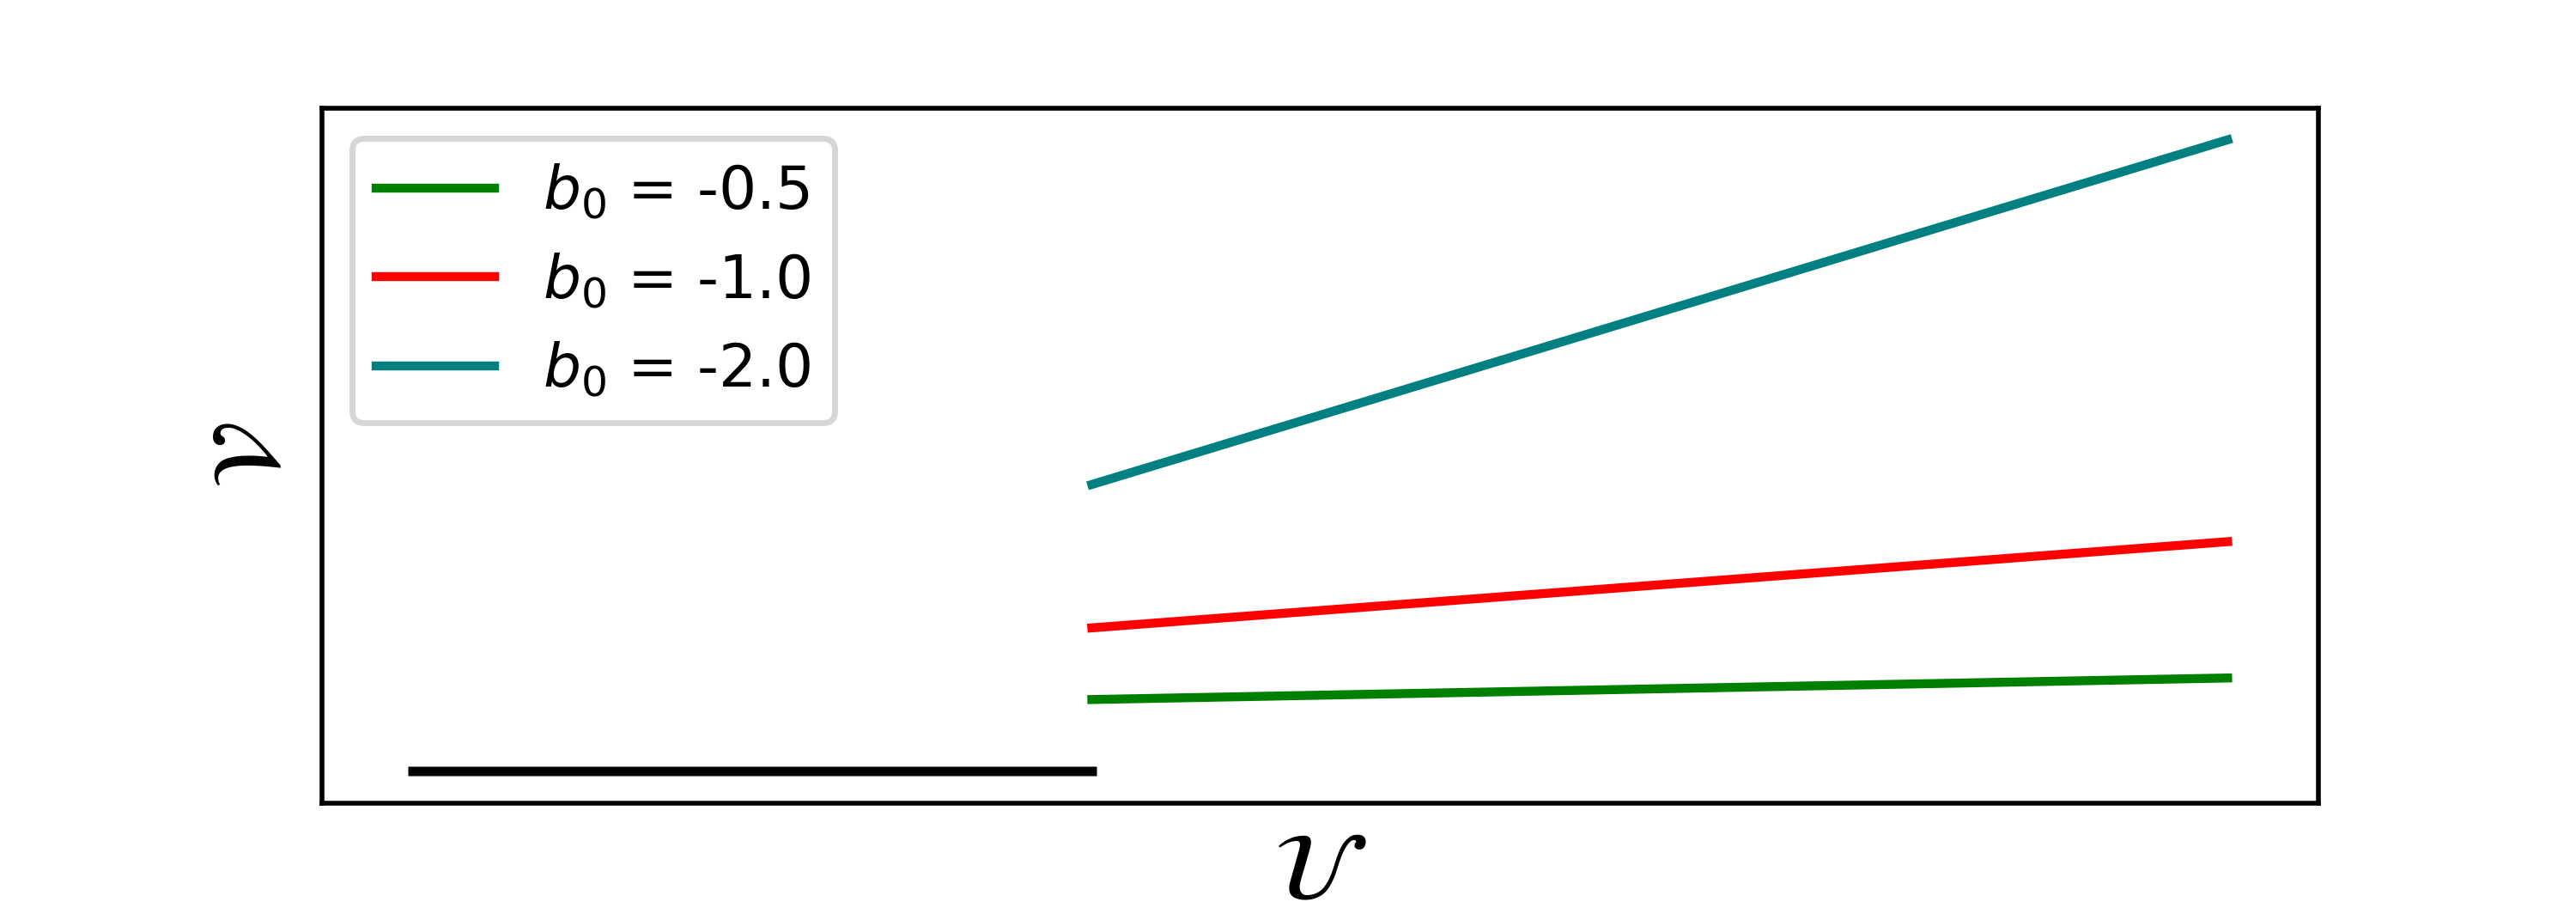
\includegraphics[width=.95\textwidth, clip]{../img/kap02/ASNullRing_UV.png}};
        \filldraw[white] (7.1,0.15) circle (10pt);
        \node[text width=12pt, anchor=north] at (7.1,0.5) {$\matu$};
        \filldraw[white] (1.3,2.3) circle (11pt);
        \node[text width=12pt, anchor=north] at (1.4,2.6) {$\matv$};
        \draw[dashed, thick, gray] (5.84,0.58) -- (5.84,4.22);
    \end{tikzpicture}
     \caption{Nulové geodetiky ($\dot \matu^-=1$, $\dot \matv^-=0$, $\dot \eta^-=0$) procházející impulzem
     AS řešení v $\rho=2$ pro různé parametry $b_0$.}
     \label{fig:Null_UV_AichelburgSexl_parameters}
\end{figure}

\begin{figure}[ht]
    \centering
    \begin{subfigure}[b]{0.45\textwidth}
        \begin{tikzpicture}
            \node[inner sep=0pt, anchor=south west] (ds) at (0,0)
            {\adjincludegraphics[trim={{.1\width} {.15\height} {.1\width} {.25\height}}, width=\textwidth, clip]{../img/kap02/ASNullRingxyUmu-1.pdf}};
            \filldraw[white] (0.59,2.65) circle (5pt);
            \node[text width=7pt] at (0.59,2.65) {\footnotesize{$\matu$}};
            \filldraw[white] (1.83,0.55) circle (5pt);
            \node[text width=7pt] at (1.82,0.55) {\footnotesize{$y$}};
            \filldraw[white] (4.7,0.55) circle (5pt);
            \node[text width=7pt] at (4.7,0.55) {\footnotesize{$x$}};
        \end{tikzpicture}
        \caption{$b_0 = -1$}
    \end{subfigure}
    \hfill
    \begin{subfigure}[b]{0.45\textwidth}
        \begin{tikzpicture}
            \node[inner sep=0pt, anchor=south west] (ds) at (0,0)
            {\adjincludegraphics[trim={{.1\width} {.15\height} {.1\width} {.25\height}}, width=\textwidth, clip]{../img/kap02/ASNullRingxyUmu-2.pdf}};
            \filldraw[white] (0.59,2.65) circle (5pt);
            \node[text width=7pt] at (0.59,2.65) {\footnotesize{$\matu$}};
            \filldraw[white] (1.83,0.55) circle (5pt);
            \node[text width=7pt] at (1.82,0.55) {\footnotesize{$y$}};
            \filldraw[white] (4.7,0.55) circle (5pt);
            \node[text width=7pt] at (4.7,0.55) {\footnotesize{$x$}};
        \end{tikzpicture}
        \caption{$b_0 = -2$}
    \end{subfigure}
    \caption{Nulové geodetiky ($\dot \matu^-=1$, $\dot \matv^-=0$, $\dot \eta^-=0$) procházející impulzní vlnou Aichelburg--Sexlova řešení. Prstenec testovacích částic je před průchodem impulzem v $\rho=2$.}
    \label{fig:NullASRing01}
\end{figure}

Záporné hodnoty parametru $b_0$, použté na obrázcích \ref{fig:Null_UV_AichelburgSexl_parameters} a \ref{fig:NullASRing01}, byly vhodné pro přehlednější vizualizaci
efektu impulzní vlny, nemají ale v originální konstrukci Aichelburg-Sexlova ultraboostu fyzikální význam. Parametr $b_0$
představuje v ultraboostové limitě $v \to 1, m \to 0$ konstantu, která splňuje $8m = b_0\sqrt{1-v^2}$, pro fyzikální systémy konstruované touto metodou
tedy nabývá kladných hodnot. Příklady nulových geodetiky pro kladné hodnoty jsou na obrázku \ref{fig:ASNullFyzikalnejsi}, kde vidíme,
že geodetiky jsou refraktovány směrem k $\rho=0$ -- jde tedy o přitažlivý efekt nulové částice generující impulzní vlnu.

\begin{figure}[ht]
    \centering
    \begin{subfigure}[b]{0.45\textwidth}
        \begin{tikzpicture}
            \node[inner sep=0pt, anchor=south west] (ds) at (0,0)
            {\adjincludegraphics[trim={{.1\width} {.1\height} {.1\width} {.25\height}}, width=\textwidth, clip]{../img/kap02/ASNullRingxyUmu1.pdf}};
            \filldraw[white] (0.59,3.1) circle (5pt);
            \node[text width=7pt] at (0.59,3.1) {\footnotesize{$\matu$}};
            \filldraw[white] (1.83,0.87) circle (5pt);
            \node[text width=7pt] at (1.82,0.87) {\footnotesize{$y$}};
            \filldraw[white] (4.7,0.85) circle (5pt);
            \node[text width=7pt] at (4.7,0.85) {\footnotesize{$x$}};
        \end{tikzpicture}
        \caption{$b_0 = 1$}
    \end{subfigure}
    \hfill
    \begin{subfigure}[b]{0.45\textwidth}
        \begin{tikzpicture}
            \node[inner sep=0pt, anchor=south west] (ds) at (0,0)
            {\adjincludegraphics[trim={{.1\width} {.1\height} {.1\width} {.25\height}}, width=\textwidth, clip]{../img/kap02/ASNullRingxyUmu2.pdf}};
            \filldraw[white] (0.59,3.1) circle (5pt);
            \node[text width=7pt] at (0.59,3.1) {\footnotesize{$\matu$}};
            \filldraw[white] (1.83,0.87) circle (5pt);
            \node[text width=7pt] at (1.82,0.87) {\footnotesize{$y$}};
            \filldraw[white] (4.7,0.85) circle (5pt);
            \node[text width=7pt] at (4.7,0.85) {\footnotesize{$x$}};
        \end{tikzpicture}
        \caption{$b_0 = 2$}
    \end{subfigure}
\caption{Nulové geodetiky ($\dot \matu^-=1$, $\dot \matv^-=0$, $\dot \eta^-=0$) procházející impulzem v $\rho=2$ pro kladné, tedy fyzikální hodnoty parametru $b_0$.}
\label{fig:ASNullFyzikalnejsi}
\end{figure}

Testovací částice s časupodobnými geodetikami se chovají stejným způsobem, na obrázku \ref{fig:AsMatter01} je vyobrazeno
šíření testovacích částic paralelně s osou $z$. Při průchodu $\matu = 0$ dochází k refrakci a částice po průchodu letí směrem k ose $z$.

\begin{figure}[H]
    \centering
    \begin{subfigure}[b]{0.45\textwidth}
        \begin{tikzpicture}
            \node[inner sep=0pt, anchor=south west] (ds) at (0,0)
        {\adjincludegraphics[trim={{.1\width} {.15\height} {.1\width} {.25\height}}, width=\textwidth, clip]{../img/kap02/ASMatterRingxyUmu0.5.pdf}};
        \filldraw[white] (0.59,2.6) circle (5pt);
        \node[text width=7pt] at (0.59,2.6) {\footnotesize{$\matu$}};
        \filldraw[white] (1.83,0.56) circle (5pt);
        \node[text width=7pt] at (1.82,0.56) {\footnotesize{$y$}};
        \filldraw[white] (4.7,0.57) circle (5pt);
        \node[text width=7pt] at (4.7,0.57) {\footnotesize{$x$}};
        \end{tikzpicture}
        \caption{$b_0 = 0.5$}
    \end{subfigure}
    \hfill
    \begin{subfigure}[b]{0.45\textwidth}
        \begin{tikzpicture}
            \node[inner sep=0pt, anchor=south west] (ds) at (0,0)
            {\adjincludegraphics[trim={{.1\width} {.15\height} {.1\width} {.25\height}}, width=\textwidth, clip]{../img/kap02/ASMatterRingxyUmu2.pdf}};
            \filldraw[white] (0.59,2.6) circle (5pt);
            \node[text width=7pt] at (0.59,2.6) {\footnotesize{$\matu$}};
            \filldraw[white] (1.83,0.56) circle (5pt);
            \node[text width=7pt] at (1.82,0.56) {\footnotesize{$y$}};
            \filldraw[white] (4.7,0.57) circle (5pt);
            \node[text width=7pt] at (4.7,0.57) {\footnotesize{$x$}};
        \end{tikzpicture}
        \caption{$b_0 = 2$}
    \end{subfigure}
    \caption{Časupodobné geodetiky ($\dot \matu^-=\frac{1}{2}$, $\dot \matv^-=1$, $\dot \eta^-=0$) procházející impulzní vlnou AS řešení. Prstenec testovacích částic je před průchodem impulzem lokalizován v $\rho=2$.}
    \label{fig:AsMatter01}
\end{figure}

Refrakce je slabší s rostoucí vzdáleností od částice generující impulz. Na obrázku \ref{fig:AS_zavislost_na_rho} jsou znázorněny už
refraktované časupodobné geodetiky pro různé vzdálenosti od osy symetrie. Před refrakcí se jedná o pohyb testovacích částic ve směru osy $z$.
Takové chování odpovídá intuitivnímu očekávání při uvážení fyzikální podstaty zdroje v AS řešení.

\begin{figure}[H]
    \centering
       \begin{tikzpicture}
           \node[inner sep=0pt, anchor=south west] (ds) at (0,0)
           {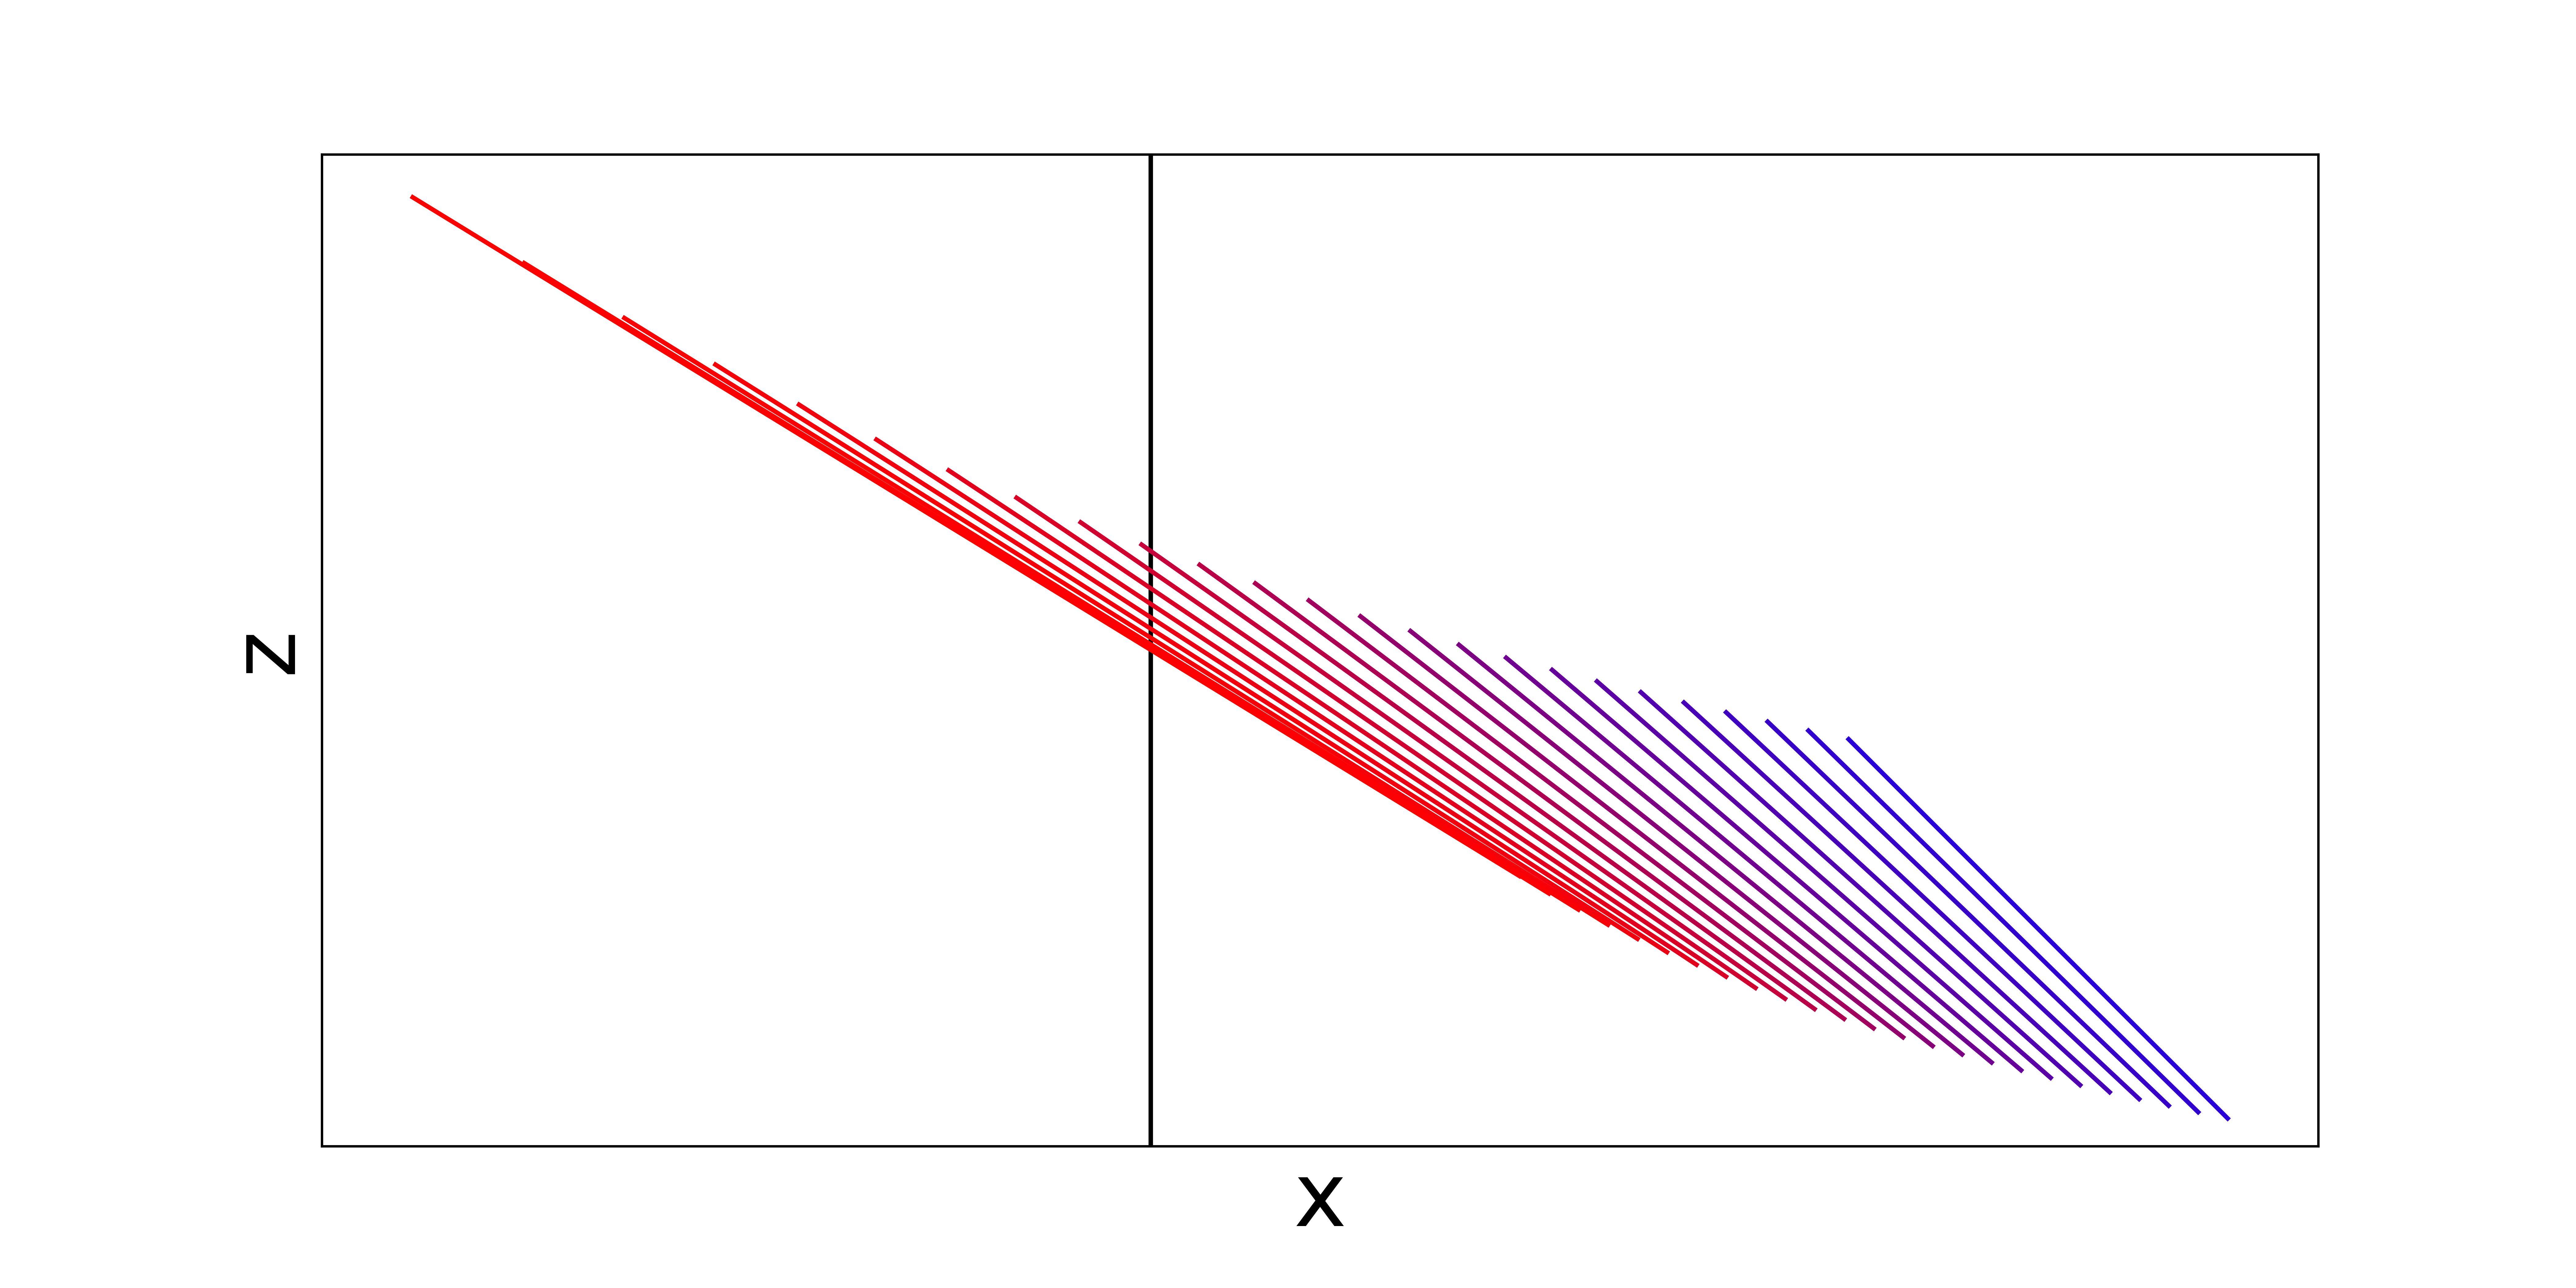
\includegraphics[width=.7\textwidth, clip]{../img/kap02/ASMatterLinexz.png}};
           \filldraw[white] (5.2,0.15) circle (9pt);
            \node[text width=10pt] at (5.2,0.15) {$x$};
            \filldraw[white] (0.9,2.4) circle (9pt);
            \node[text width=10pt] at (1,2.4) {$z$};
        \end{tikzpicture}
    \caption{Refraktované časupodobné geodetiky po průchodu impulzem v různých vzdálenostech $\rho$ pro $b_0 = \frac{1}{2}$.
    Červená barva odpovídá částici refraktované nejblíže ($\rho=\frac{1}{2}$), modrá nejdále ($\rho = 2$). Černá přímka odpovídá
    ose $x=0$.}
    \label{fig:AS_zavislost_na_rho}
\end{figure}


Pro potěšení oka čtenáře jsou přiloženy další vizualizace geodetického pohybu v Aichelburg-Sexlově řešení. Na obrázku \ref{fig:AsMatter02} je systém časupodobných geodetik, které se před
průchodem impulzní vlnou šíří směrem od osy symetrie $z$. V (b) dochází k refrakci, která otáčí směr šíření směrem zpět k ose $z$.
Na obrázku \ref{fig:AsMatterNonAxial} je pak zobrazení průchodu geodetik, které nejsou uspořádány axiálně symetricky.

\begin{figure}[H]
    \centering
    \begin{subfigure}[b]{0.45\textwidth}
        \begin{tikzpicture}
            \node[inner sep=0pt, anchor=south west] (ds) at (0,0)
            {\adjincludegraphics[trim={{.1\width} {.15\height} {.1\width} {.25\height}}, width=\textwidth, clip]{../img/kap02/ASMatterRing_XYMOVING__xyU_mu2.pdf}};
            \filldraw[white] (0.59,2.7) circle (5pt);
            \node[text width=7pt] at (0.59,2.7) {\footnotesize{$\matu$}};
            \filldraw[white] (1.83,0.54) circle (5pt);
            \node[text width=7pt] at (1.82,0.54) {\footnotesize{$y$}};
            \filldraw[white] (4.7,0.57) circle (5pt);
            \node[text width=7pt] at (4.7,0.57) {\footnotesize{$x$}};
        \end{tikzpicture}
        \caption{$b_0 = 2$}
    \end{subfigure}
    \hfill
    \begin{subfigure}[b]{0.45\textwidth}
        \begin{tikzpicture}
            \node[inner sep=0pt, anchor=south west] (ds) at (0,0)
            {\adjincludegraphics[trim={{.1\width} {.15\height} {.1\width} {.25\height}}, width=\textwidth, clip]{../img/kap02/ASMatterRing_XYMOVING__xyU_mu4.pdf}};
            \filldraw[white] (0.59,2.7) circle (5pt);
            \node[text width=7pt] at (0.59,2.7) {\footnotesize{$\matu$}};
            \filldraw[white] (1.83,0.54) circle (5pt);
            \node[text width=7pt] at (1.82,0.54) {\footnotesize{$y$}};
            \filldraw[white] (4.7,0.57) circle (5pt);
            \node[text width=7pt] at (4.7,0.57) {\footnotesize{$x$}};
        \end{tikzpicture}
        \caption{$b_0 = 4$}
    \end{subfigure}
    \caption{Časupodobné geodetiky ($\dot \matu^-=1$, $\dot \matv^-=2$, $\dot \eta^-=\sqrt{\frac{3}{2}} e^{i \phi}$), kde $\phi$ odpovídá úhlu v
    cylindrických souřadnicích, ve kterém částice leží, procházející impulzní vlnou AS řešení v $\rho=2$.}
    \label{fig:AsMatter02}
\end{figure}

\begin{figure}[H]
    \centering
    \begin{tikzpicture}
        \node[inner sep=0pt, anchor=south west] (ds) at (0,0)
        {\adjincludegraphics[trim={{.1\width} {.15\height} {.1\width} {.22\height}}, width=0.8\textwidth, clip]{../img/kap02/ASMatterHearthxyUmu1.pdf}};
        \filldraw[white] (1.87,2.7) circle (9pt);
        \node[text width=9pt] at (1.87,2.7) {\small{$\matu$}};
        \filldraw[white] (8.8,2.7) circle (10pt);
        \node[text width=7pt] at (8.8,2.7) {\small{$y$}};
        \filldraw[white] (5,0.57) circle (10pt);
        \node[text width=7pt] at (5,0.57) {\small{$x$}};
    \end{tikzpicture}
    \caption{Časupodobné geodetiky ($\dot \matu^-=\frac{1}{2}$, $\dot \matv^-=1$, $\dot \eta^-=0$) ve vybraném uspořádání procházející nadplochou $\matu = 0$.}
    \label{fig:AsMatterNonAxial}
\end{figure}
Pro $m>0$ závisí změna geodetického pohybu na prostorovém úhlu. Derivace profilové funkce $H_{i,Z}$, která vystupuje v refrakčních rovnicích, je pro jednotlivá $m$
\begin{equation}
    H_{i,Z}^{(m)}(\eta, \bar{\eta}) = -\frac{(\sqrt{2})^{m} b_m m}{\eta^{m+1}}.
\end{equation}
Speciálně pro $m=1$, tedy impulz generovaný částicí s dipólovou strukturou, je $H_{i,Z}^{(1)}$ vykreslena na obrázku \ref{fig:DipoleHZ}. Reálná část a imaginární část
odpovídá derivacím ve směru $X$ a $Y$ vystupujícím v refrakčních rovnicích \eqref{eq:refraction_velocity_null_cart} - přímo tedy ukazují závislost změny čtyřrychlosti v těchto směrech na místě průchodu geodetiky vlnoplochou,

\begin{equation}
    \begin{split}
        \Re(H_{i,Z}) &= \frac{1}{\sqrt{2}} H_{i,X}, \\
        \Im(H_{i,Z}) &=-\frac{1}{\sqrt{2}}H_{i,Y}.
    \end{split}
\end{equation}


Příklad nulových geodetik procházejících impulzem s jediným nenulovým členem pro $m=1$ je na obrázku \ref{fig:DipoleAxial}, pro časupodobné geodetiky dostáváme totožné
chování (viz obrázek \ref{fig:DipoleAxialTimelike})

\begin{figure}[ht]
    \centering
    \begin{subfigure}[b]{0.48\textwidth}
        \begin{tikzpicture}
            \node[inner sep=0pt, anchor=south west] (ds) at (0,0)
        {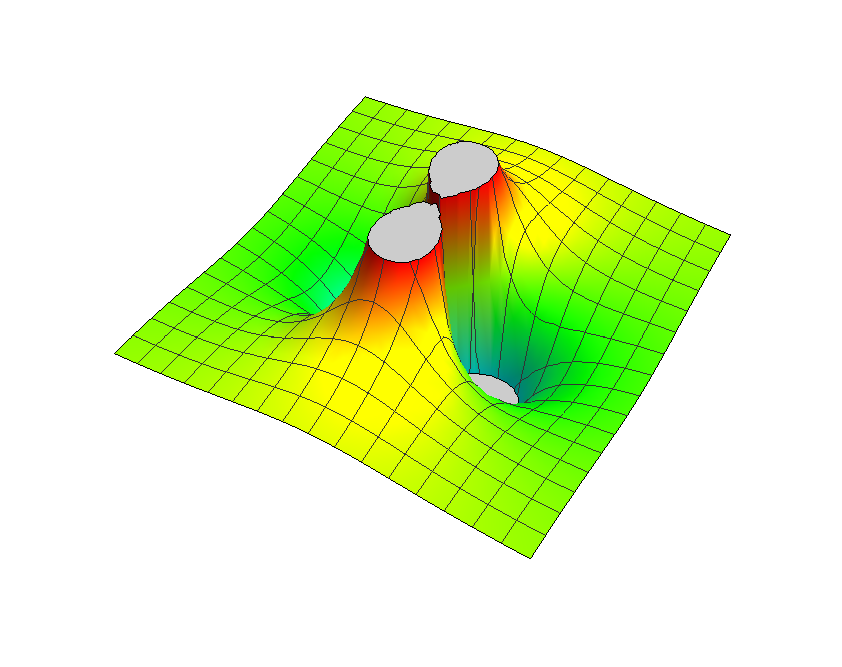
\includegraphics[width=1\textwidth, clip]{../img/kap02/DipoleHZReal.pdf}};
        \end{tikzpicture}
        \caption{$\Re(H_{i,Z}^{(1)})$}
    \end{subfigure}
    \hfill
    \begin{subfigure}[b]{0.48\textwidth}
        \begin{tikzpicture}
            \node[inner sep=0pt, anchor=south west] (ds) at (0,0)
            {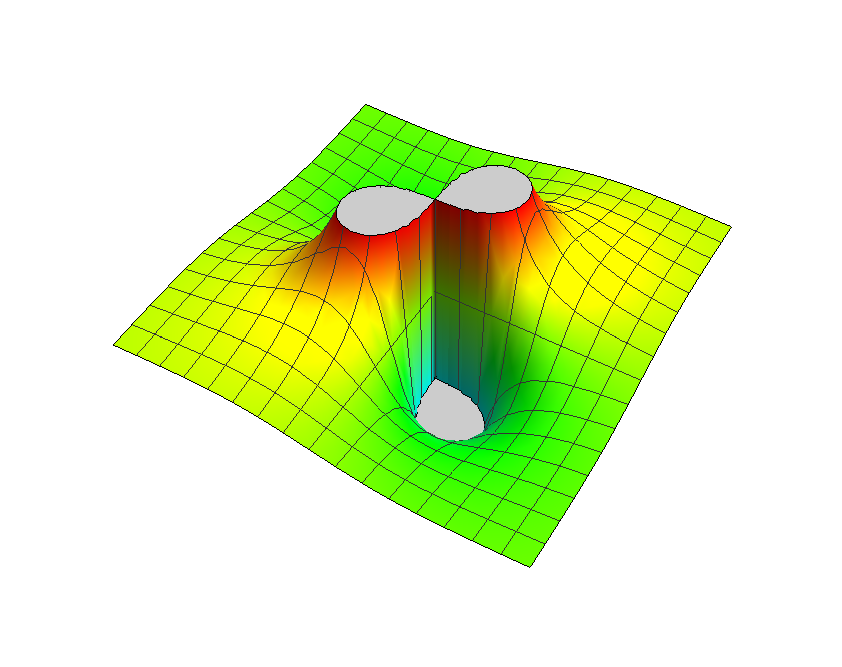
\includegraphics[width=1\textwidth, clip]{../img/kap02/DipoleHZImaginary.pdf}};
        \end{tikzpicture}
        \caption{$\Im(H_{i,Z}^{(1)})$}
    \end{subfigure}
    \caption{Reálná a imaginární část funkce profilu vlny $H_{i,Z}^{(1)}(x, y)$.}
    \label{fig:DipoleHZ}
\end{figure}
\begin{figure}[ht]
    \centering
    \begin{tikzpicture}
        \node[inner sep=0pt, anchor=south west] (ds) at (0,0)
        {\adjincludegraphics[trim={{.1\width} {.15\height} {.1\width} {.22\height}}, width=0.8\textwidth, clip]{../img/kap02/DipoleNullxyUb1_0.2.pdf}};
        \filldraw[white] (9.2,2) circle (9pt);
        \node[text width=9pt] at (9.2,2) {\small{$\matu$}};
        \filldraw[white] (2,4.92) circle (6pt);
        \node[text width=7pt] at (2,4.92) {\small{$x$}};
        \node at (5.8,1.083) [rectangle,draw, white, fill=white] {$y$};
        \node[text width=7pt] at (5.8,1.13) {\small{$y$}};
    \end{tikzpicture}    
    \caption{Nulové geodetiky ($\dot \matu^-=1$, $\dot \matv^-=0$, $\dot \eta^-=0$) v axiálně symetrickém uspořádání ($\rho=1$) na $\mathcal{M}^-$ procházející impulzní nadplochou vlny generované částicí s dipólovou strukturou
    s parametrem $b_1=0.2$.}
    \label{fig:DipoleAxial}
\end{figure}
\begin{figure}[ht]
    \centering
    \begin{tikzpicture}
        \node[inner sep=0pt, anchor=south west] (ds) at (0,0)
        {\adjincludegraphics[trim={{.1\width} {.15\height} {.1\width} {.22\height}}, width=0.8\textwidth, clip]{../img/kap02/DipoleTimelikexyUb1_0.4.pdf}};
        \filldraw[white] (9.2,2) circle (9pt);
        \node[text width=9pt] at (9.2,2) {\small{$\matu$}};
        \filldraw[white] (2,4.92) circle (6pt);
        \node[text width=7pt] at (2,4.92) {\small{$x$}};
        \node at (5.8,1.083) [rectangle,draw, white, fill=white] {$y$};
        \node[text width=7pt] at (5.8,1.13) {\small{$y$}};
    \end{tikzpicture}    
    \caption{Časupodobné geodetiky ($\dot \matu^-=0.5$, $\dot \matv^-=1$, $\dot \eta^-=0$) v axiálně symetrickém uspořádání ($\rho=1$) na $\mathcal{M}^-$ procházející impulzní nadplochou vlny generované částicí s dipólovou strukturou,
    s parametrem $b_1=0.4$.}
    \label{fig:DipoleAxialTimelike}
\end{figure}
\clearpage

\subsection{Impulzní gravitační vlna generovaná nehmotnými částicemi s multipólovou strukturou s \texorpdfstring{$\Lambda\neq 0$}{Lambda =/= 0}}

V prostoročasech s nenulovou konstantou odvodili Griffiths a Podolský \cite{Podolsky1997} tvar řešení obdobný \eqref{eq:multipole_minkowski},
tedy případ impulzních vln generovaných nulovými částicemi s multipólovou strukturou. Vyšli z redukce Einsteinových rovnic pro distribuční
metriku \eqref{eq:5DDistributionalWaveMetric}. V případě ryze gravitačních vln dostáváme podmínku
\begin{equation}
    \label{eq:podminka_na_H_lambda_stare}
    \left(\Delta + \frac{2}{3} \Lambda \right)\mathcal{H} = 0,
\end{equation}
kde $\Delta$ je Laplaceův operátor působící na impulzní nadploše. Při parametrizaci 
\begin{equation}
    \begin{split}
        Z_2 &= a \sqrt{\epsilon(1-z^2)} \cos \phi,\\
        Z_3 &= a \sqrt{\epsilon(1-z^2)} \sin \phi,\\
        Z_4 &= a~z,
    \end{split}
\end{equation}
kde pro $\Lambda > 0$ je $\left|z\right| \leq 1$ a pro $\Lambda < 0$ je $\left|z\right| \geq 1$,
nabývá funkce $\mathcal{H}(z, \phi)$ tvaru
\begin{equation}
    \mathcal{H}(z, \phi) = b_0 Q_1(z) + \sum_{m=1}^\infty b_0 Q_1^m(z) \cos [m(\phi - \phi_m)],
\end{equation}
kde $Q_1^m(z)$ jsou přidružené Legendrovy funkce druhého druhu, tedy
\begin{equation}
    Q_1^m(z) = -(\epsilon)^m |1-z^2|^{m/2} \frac{d^m}{dz^m}Q_1(z).
\end{equation}

První člen
\begin{equation}
    b_0 Q_1(z) = b_0 \left(\frac{z}{2} \log \left|\frac{1+z}{1-z}\right| - 1\right)
\end{equation}
představuje axiálně symetrické Hottovo--Tanakovo řešení \cite{Hotta_1993}, které odpovídá boostu Schwarzschildova--(anti--)de Sitterova
prostoročasu. Toto řešení je analogií Aichelburg--Sexlova řešení v (anti--)de Sitterově prostoročasu se singulární hmotou generující vlnu v $z=1$. V případě de Sitterova prostoročasu je impulzní nadplocha
neexpandující sféra generovaná dvěma nehmotnými částicemi, které letí v opačném směru. V anti--de Sitterově prostoročasu je impulzní nadplocha hyperboloidální
plochou generovaná částicí, která se (díky tomu, že se jedná o nakrytí $\mathbb{R}^4$ s topologií $\mathbb{S}^1 \times \mathbb{R}^3$) periodicky pohybuje mezi prostorovými nekonečny,
z jedné strany na druhou.

Na obrázku \ref{fig:funkceHhodnotyvADS} vidíme hodnoty funkce $\mathcal{H}(Z_2, Z_3, Z_4)$ Hottova--Tanakova řešení na vlnoploše v (A--)dS prostoročasu (s $|\Lambda | = 1$).

\begin{figure}[ht]
    \centering
    \begin{subfigure}[b]{0.45\textwidth}
        \begin{tikzpicture}
            \node[inner sep=0pt, anchor=south west] (ds) at (0,0)
        {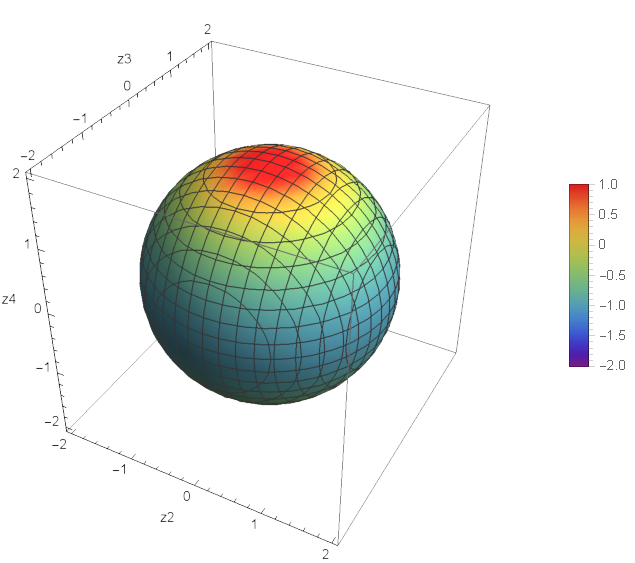
\includegraphics[width=1\textwidth, clip]{../img/kap02/dSWaveFrontHValue.pdf}};
        \end{tikzpicture}
        \caption{de Sitterův prostoročas}
    \end{subfigure}
    \hfill
    \begin{subfigure}[b]{0.45\textwidth}
        \begin{tikzpicture}
            \node[inner sep=0pt, anchor=south west] (ds) at (0,0)
            {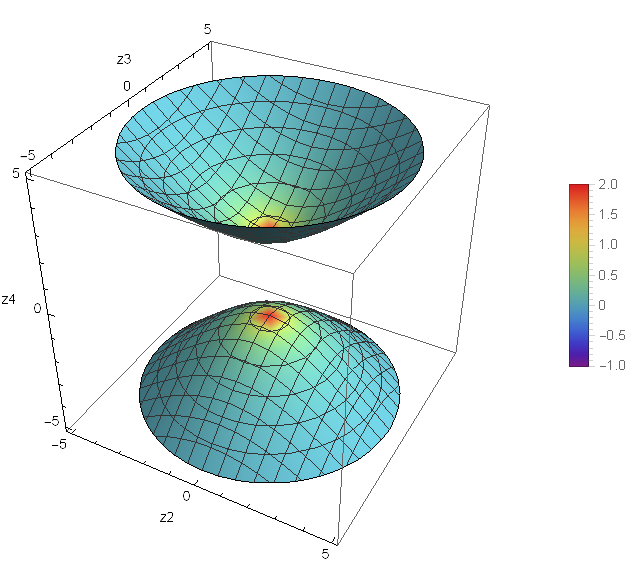
\includegraphics[width=1\textwidth, clip]{../img/kap02/AdSWaveFrontHValue.pdf}};
        \end{tikzpicture}
        \caption{anti--de Sitterův prostoročas}
    \end{subfigure}
    \caption{Funkce $\mathcal{H}$ má v de Sitterově prostoročasu singulární body na pólech sféry odpovídající vlnoploše ($Z_4 = \pm a$), v anti--de Sitterově
    prostoročase singularity leží na vrcholech hyperboloidálních vlnoploch.}
    \label{fig:funkceHhodnotyvADS}
\end{figure}

Geodetický pohyb nulových částic je v konformně plochých souřadnicích
nezávislý na hodnotě kosmologické konstanty, chování na impulzní ploše se pak liší pouze ve tvaru příslušné funkce $H(\eta, \bar{\eta})$, která má v případě Hottova--Tanakova řešení
v konformně plochých souřadnicích tvar
\begin{equation}
    \label{eq:Hotta_Tanaka_H_conf_flat_coords}
    H(\eta, \bar{\eta}) = \frac{1}{24} b_0 \left((\Lambda \eta \bar{\eta} + 6) \log \left(\left| \frac{6}{\Lambda \eta \bar{\eta} }\right| \right)+2 (\Lambda \eta \bar{\eta} - 6)\right),
\end{equation}
a v derivacích $H$ ve směru $\eta$, respektive $\bar{\eta}$.

Jako první ukážeme pohyb nulových částic v nadploše $y=0$ (to znamená, že souřadnice $\eta$ je reálná). Díky axiální symetrii tak zároveň prozkoumáme
vlastnosti nulových geodetik ve všech nadplochách obsahujících osu této symetrie.
Tento pohyb je pro řešení s $b_0 = 1$ zobrazen v konformně plochých souřadnicích  na obrázku \ref{fig:HottaTanakaNullY0}.

\begin{figure}[ht]
    \centering
    \begin{subfigure}[b]{0.45\textwidth}
        \begin{tikzpicture}
            \node[inner sep=0pt, anchor=south west] (ds) at (0,0)
            {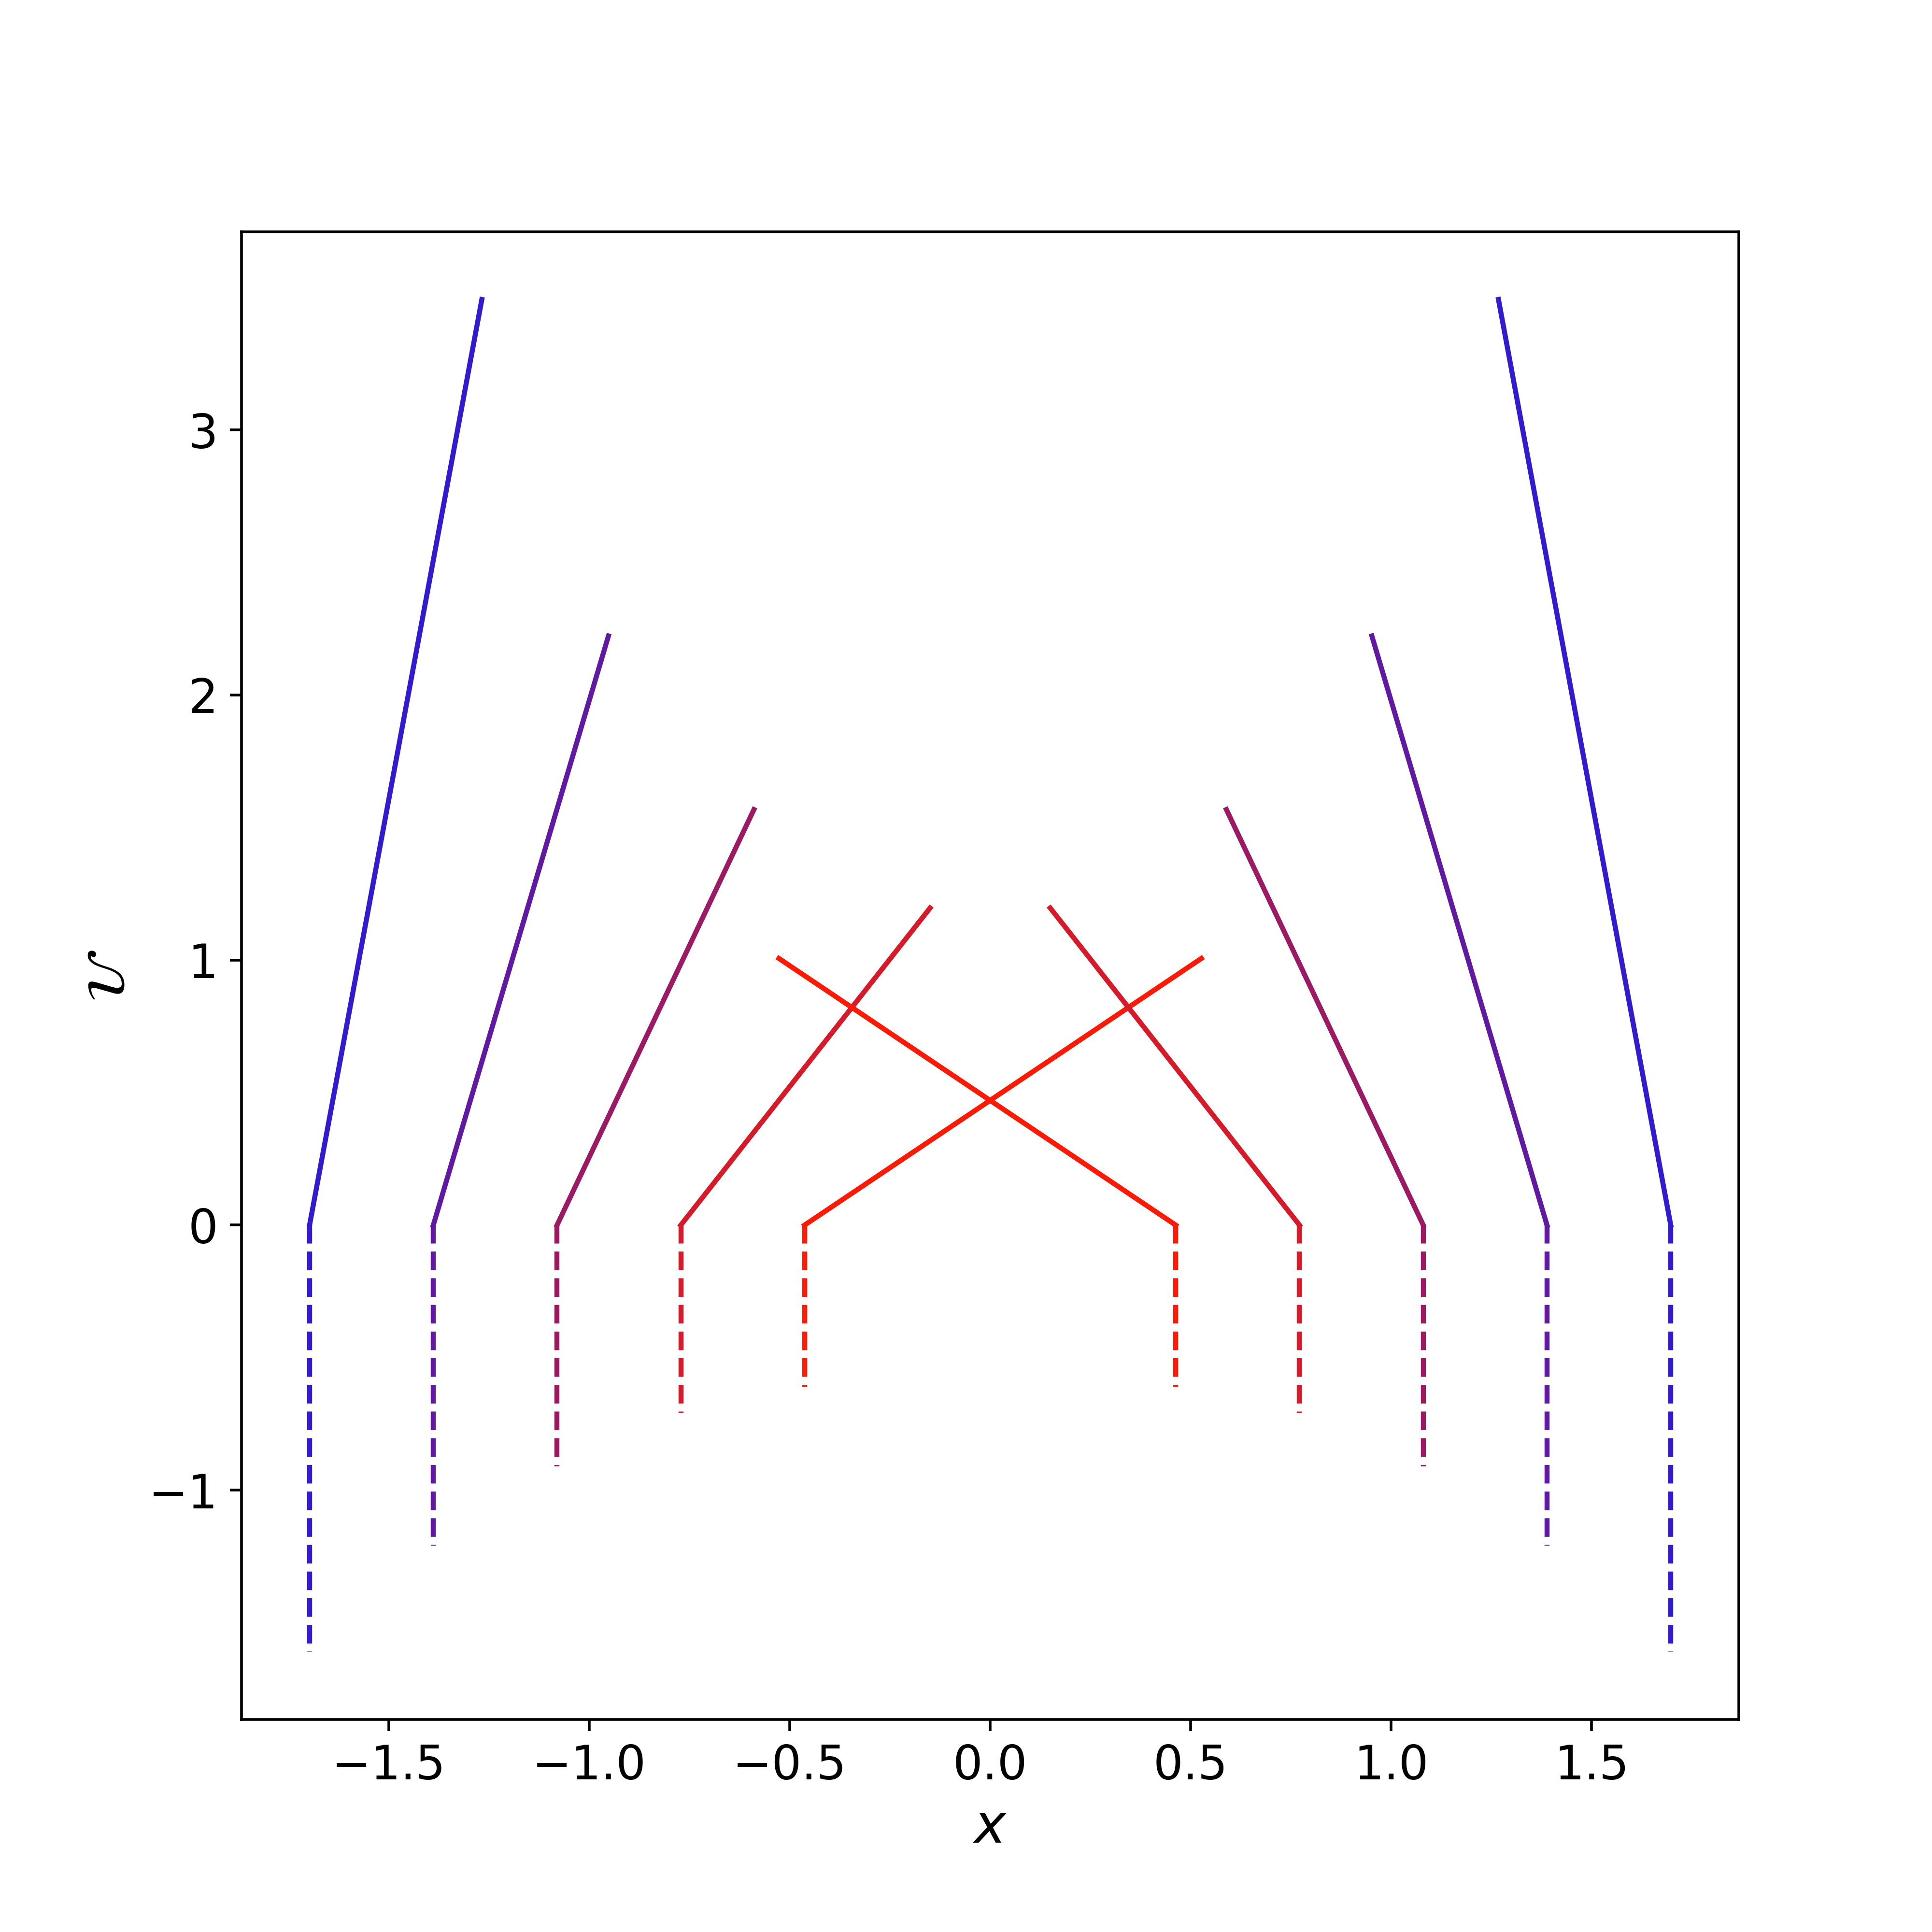
\includegraphics[width=.95\textwidth, clip]{../img/kap02/HT_y-0__xU_mu1_lmb1.png}};
            \filldraw[white] (0.29,3.1) circle (4pt);
            \node[text width=7pt] at (0.29,3.1) {\scriptsize{$\matu$}};
            \filldraw[white] (3.25,0.28) circle (4pt);
            \node[text width=7pt] at (3.25,0.28) {\scriptsize{$x$}};
        \end{tikzpicture}
        \caption{$\Lambda = 1$}
    \end{subfigure}
    \hfill
    \begin{subfigure}[b]{0.45\textwidth}
        \begin{tikzpicture}
            \node[inner sep=0pt, anchor=south west] (ds) at (0,0)
            {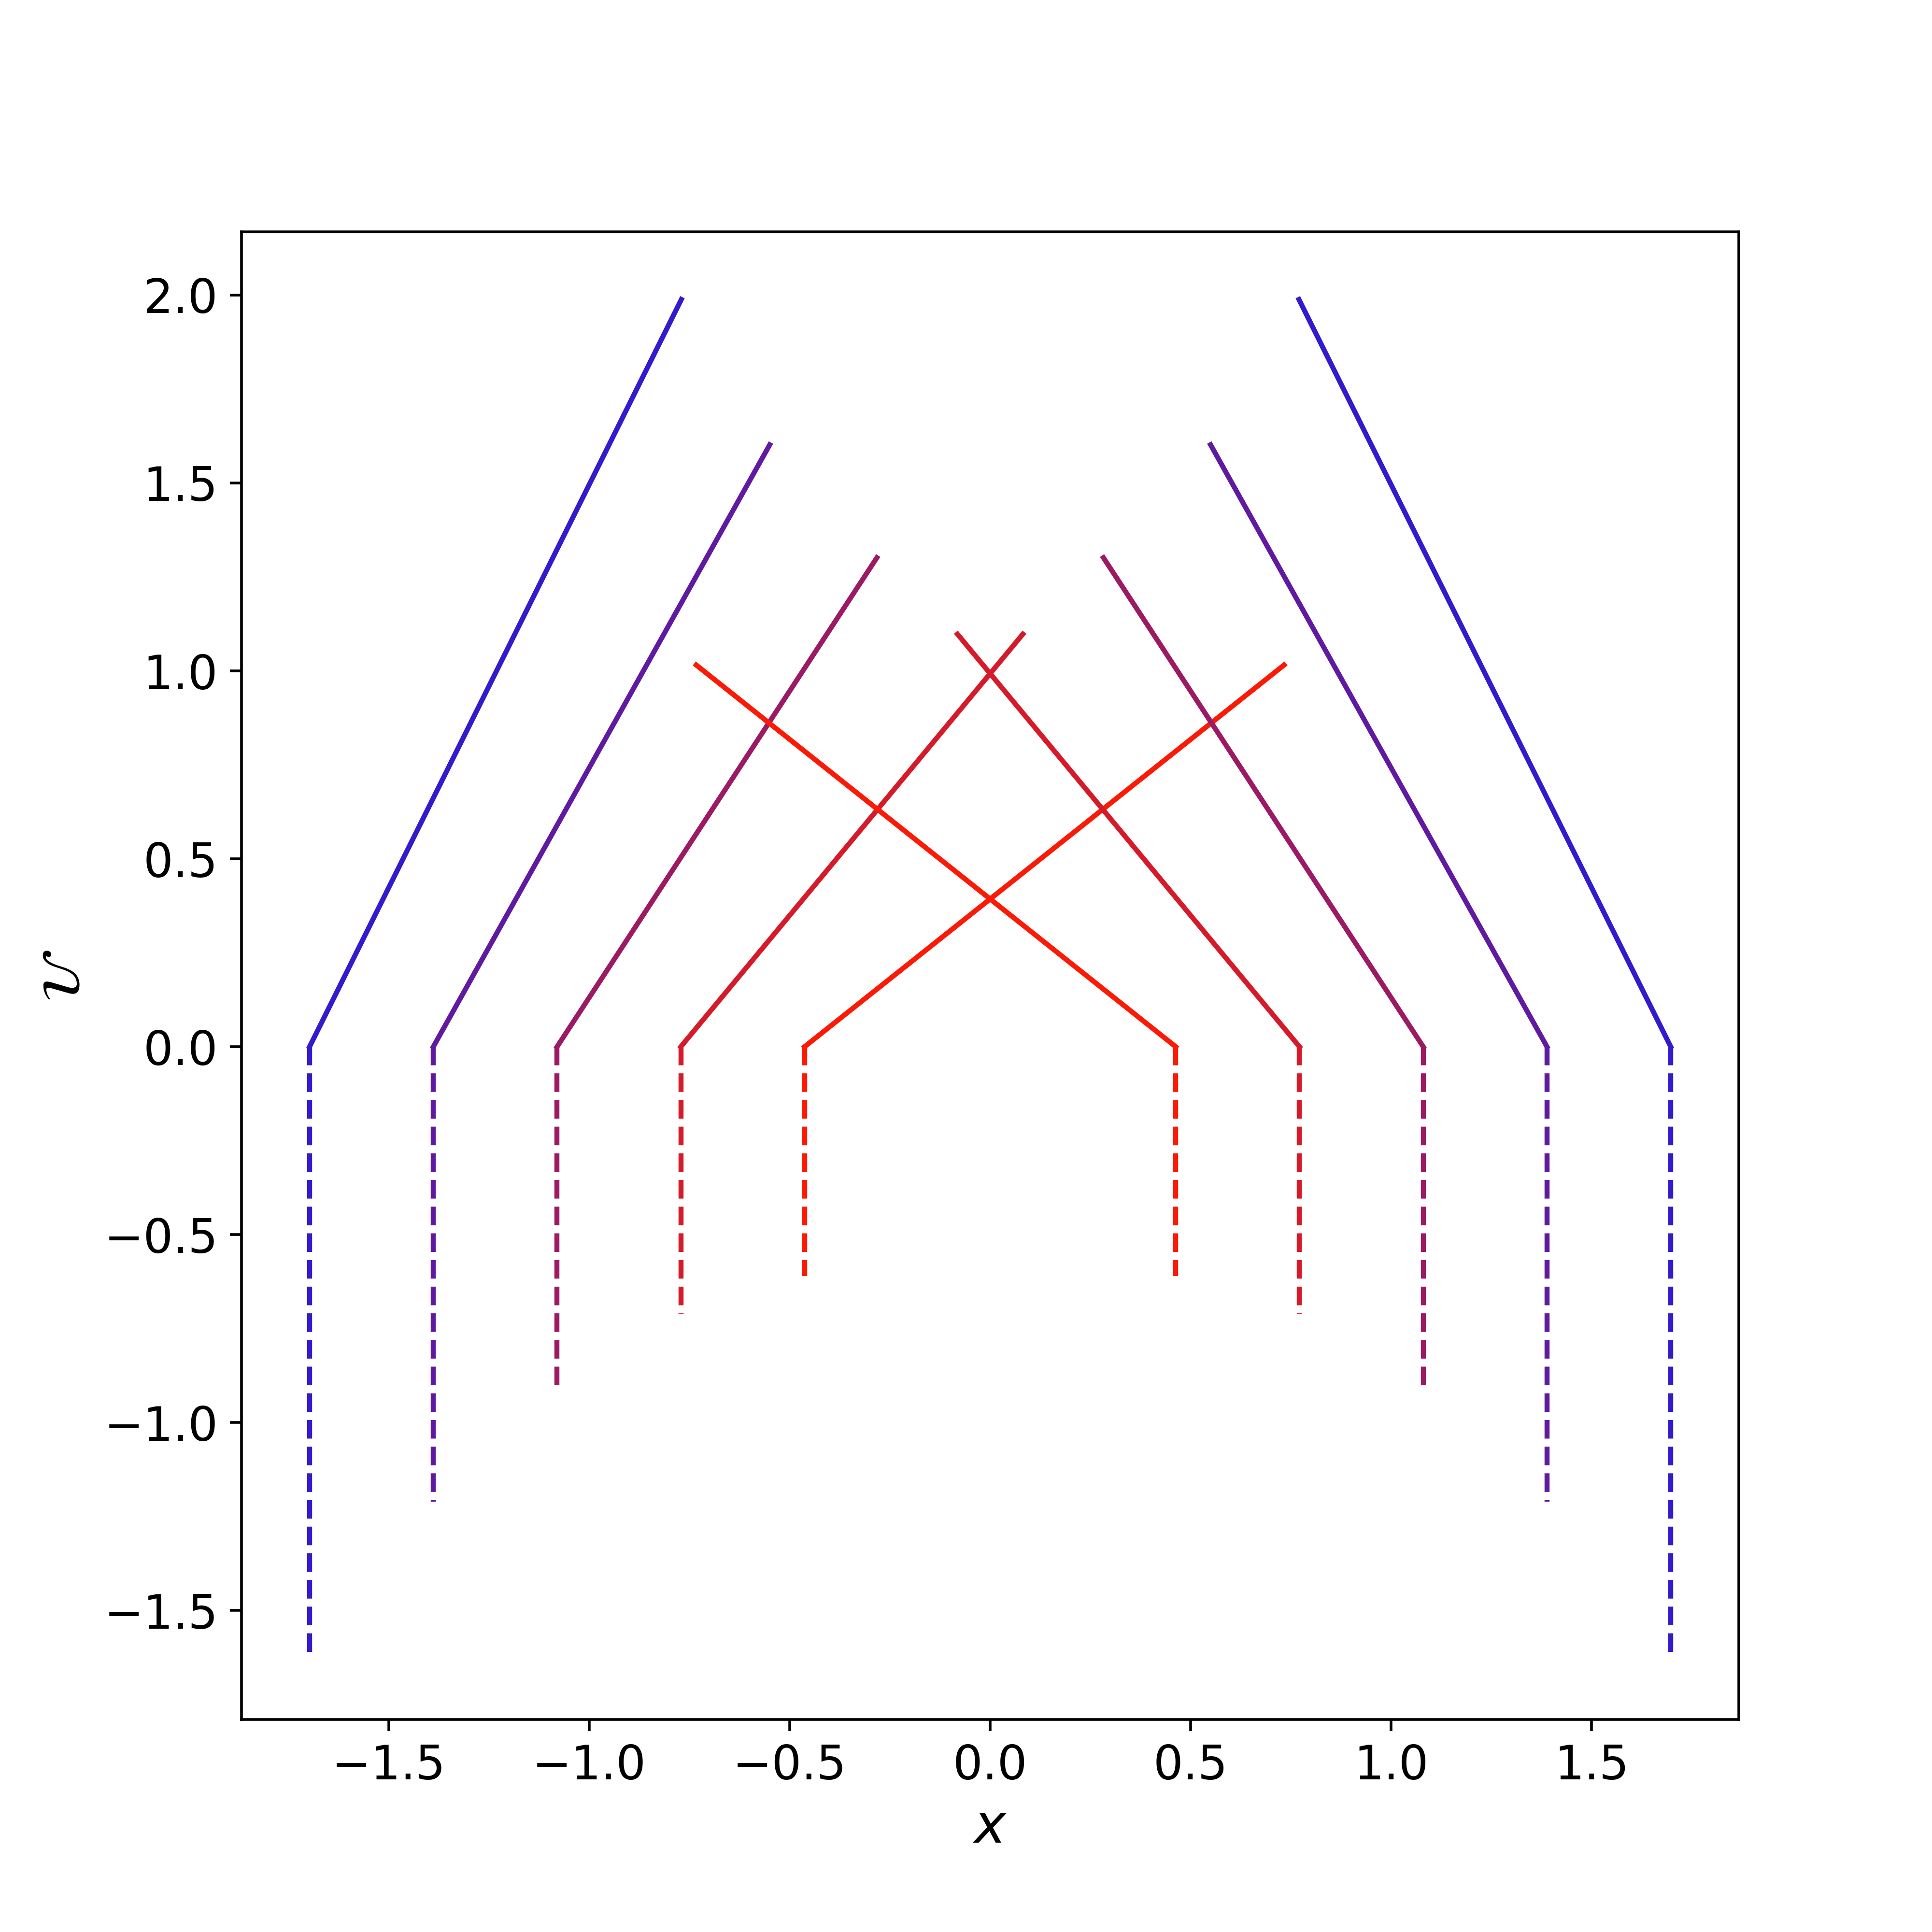
\includegraphics[width=.95\textwidth, clip]{../img/kap02/HT_y-0__xU_mu1_lmb-1.png}};
            \filldraw[white] (0.29,3.1) circle (4pt);
            \node[text width=7pt] at (0.29,3.1) {\scriptsize{$\matu$}};
            \filldraw[white] (3.25,0.28) circle (4pt);
            \node[text width=7pt] at (3.25,0.28) {\scriptsize{$x$}};
        \end{tikzpicture}
        \caption{$\Lambda = -1$}
    \end{subfigure}

    \begin{subfigure}[b]{0.45\textwidth}
        \begin{tikzpicture}
            \node[inner sep=0pt, anchor=south west] (ds) at (0,0)
            {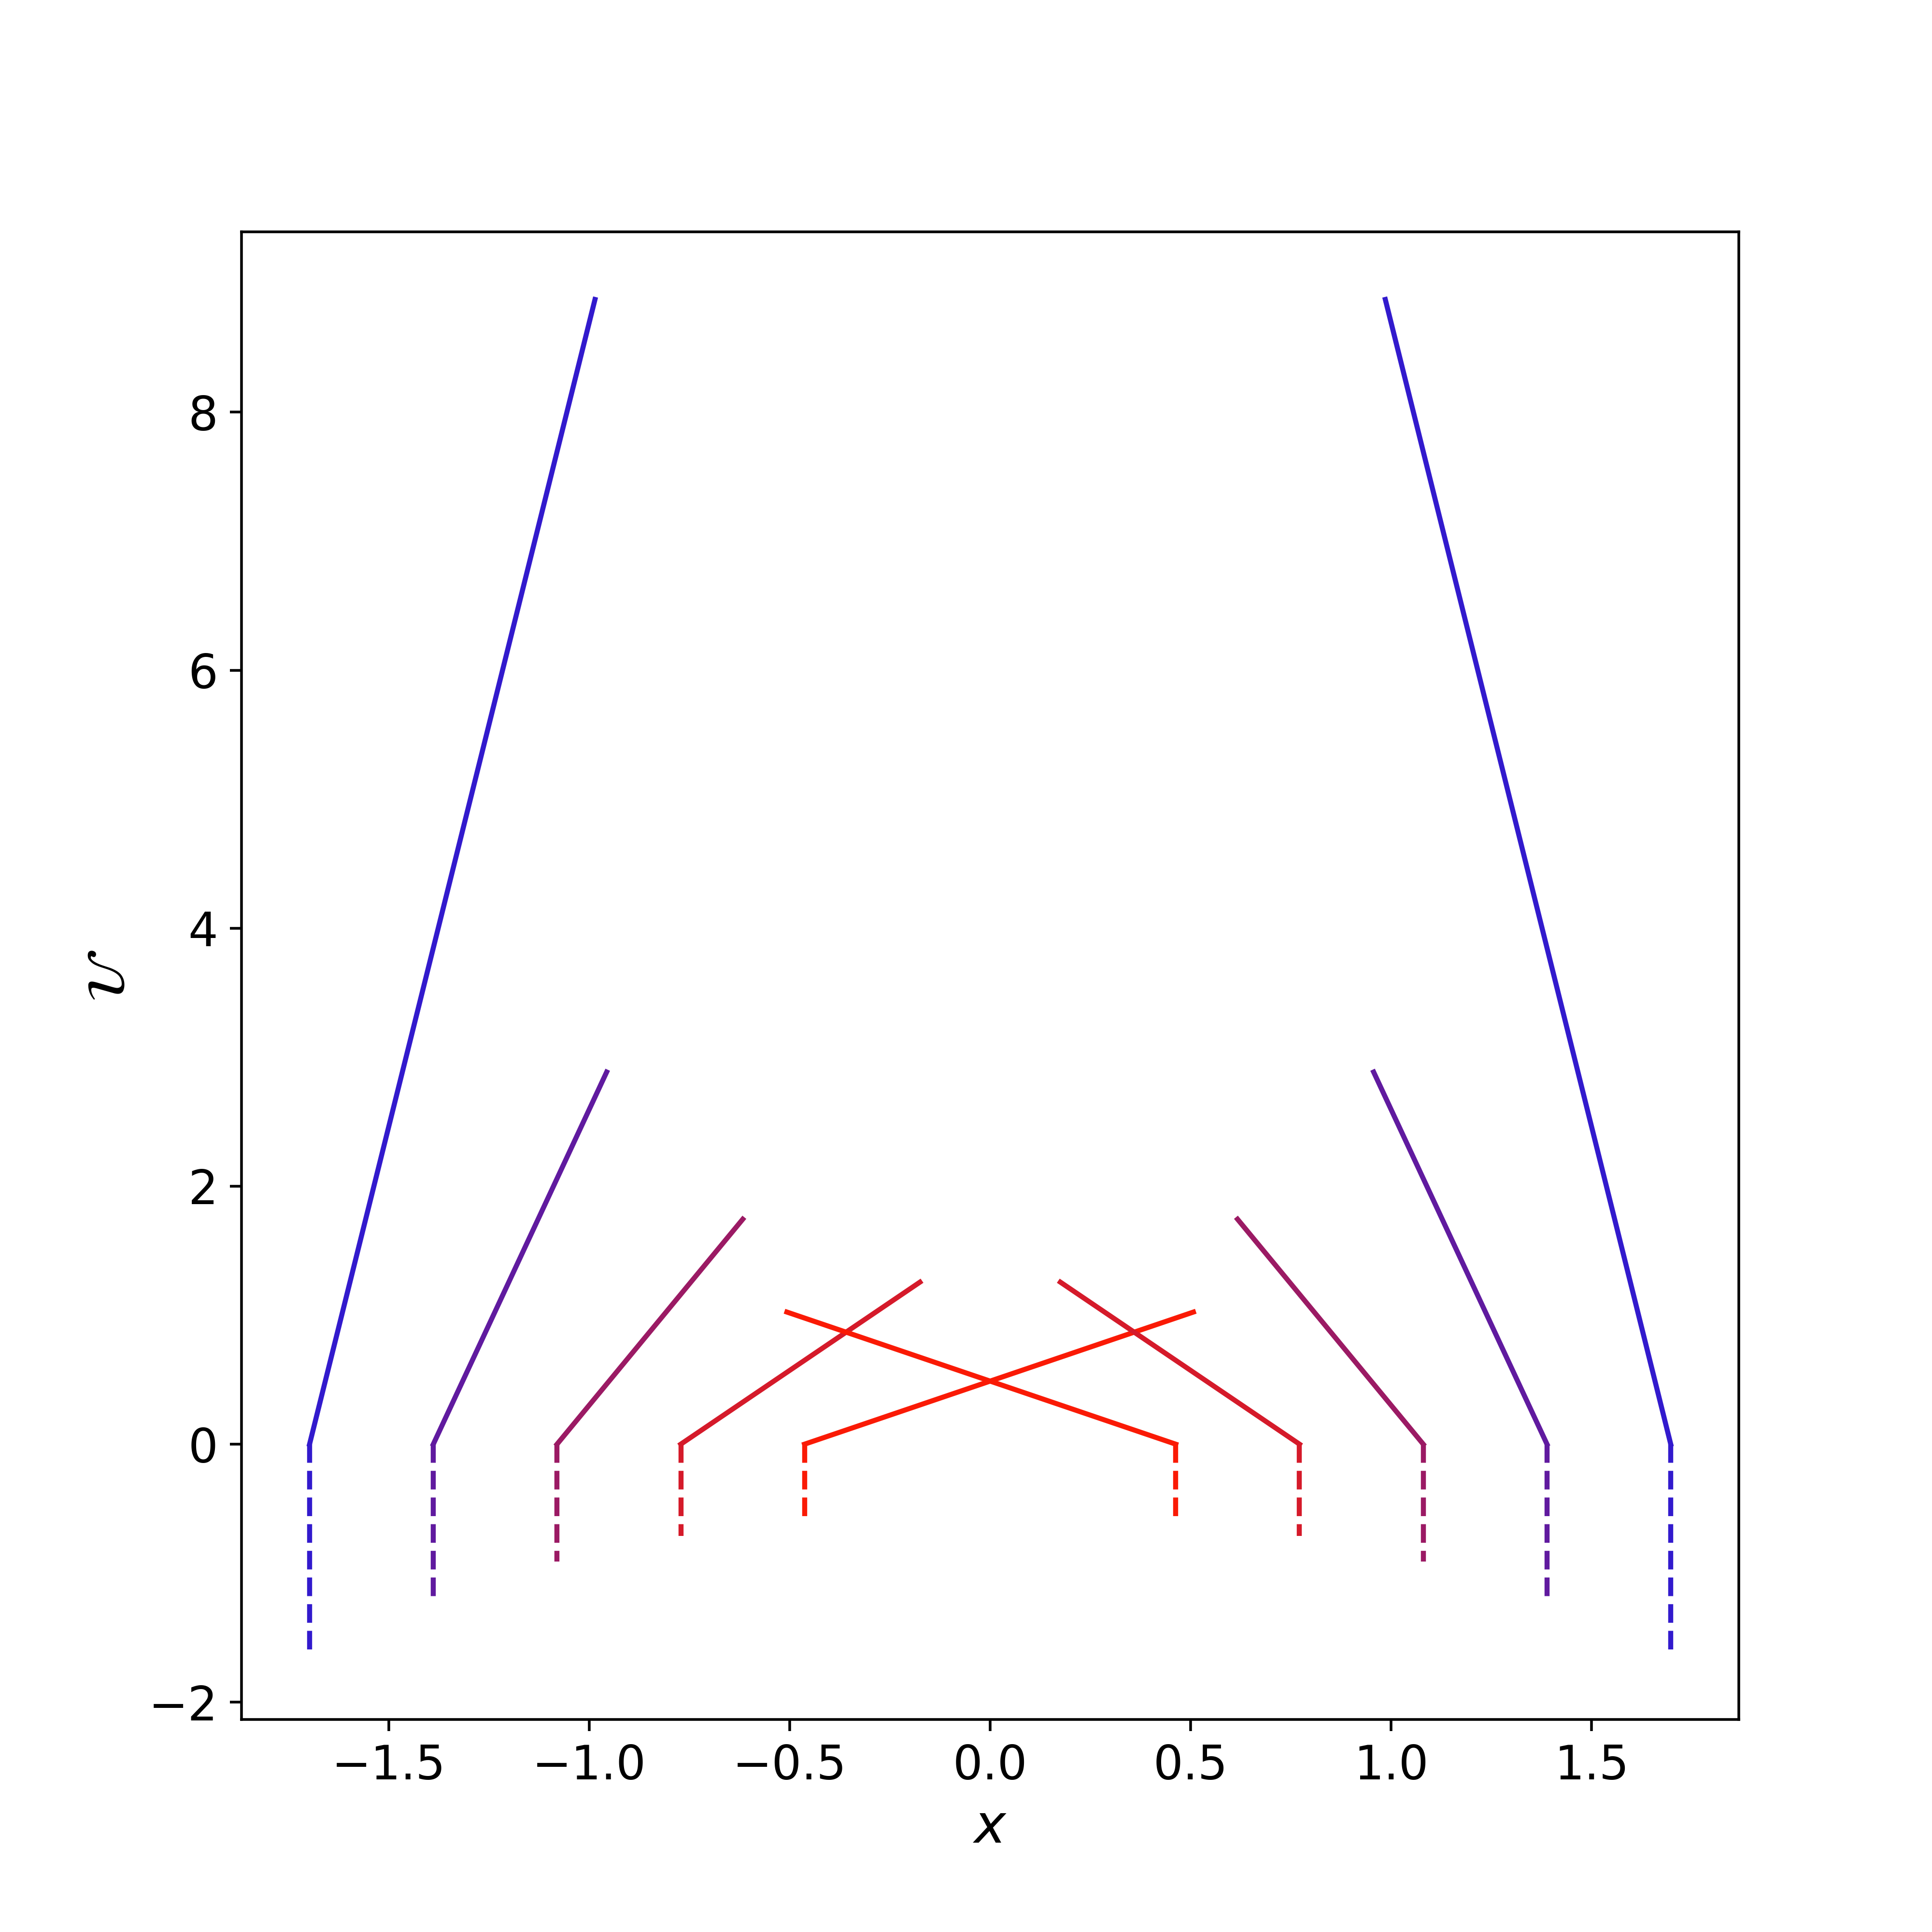
\includegraphics[width=.95\textwidth, clip]{../img/kap02/HT_y-0__xU_mu1_lmb1,5.png}};
            \filldraw[white] (0.29,3.1) circle (4pt);
            \node[text width=7pt] at (0.29,3.1) {\scriptsize{$\matu$}};
            \filldraw[white] (3.25,0.28) circle (4pt);
            \node[text width=7pt] at (3.25,0.28) {\scriptsize{$x$}};
        \end{tikzpicture}
        \caption{$\Lambda = 1,5$}
    \end{subfigure}
    \hfill
    \begin{subfigure}[b]{0.45\textwidth}
        \begin{tikzpicture}
            \node[inner sep=0pt, anchor=south west] (ds) at (0,0)
            {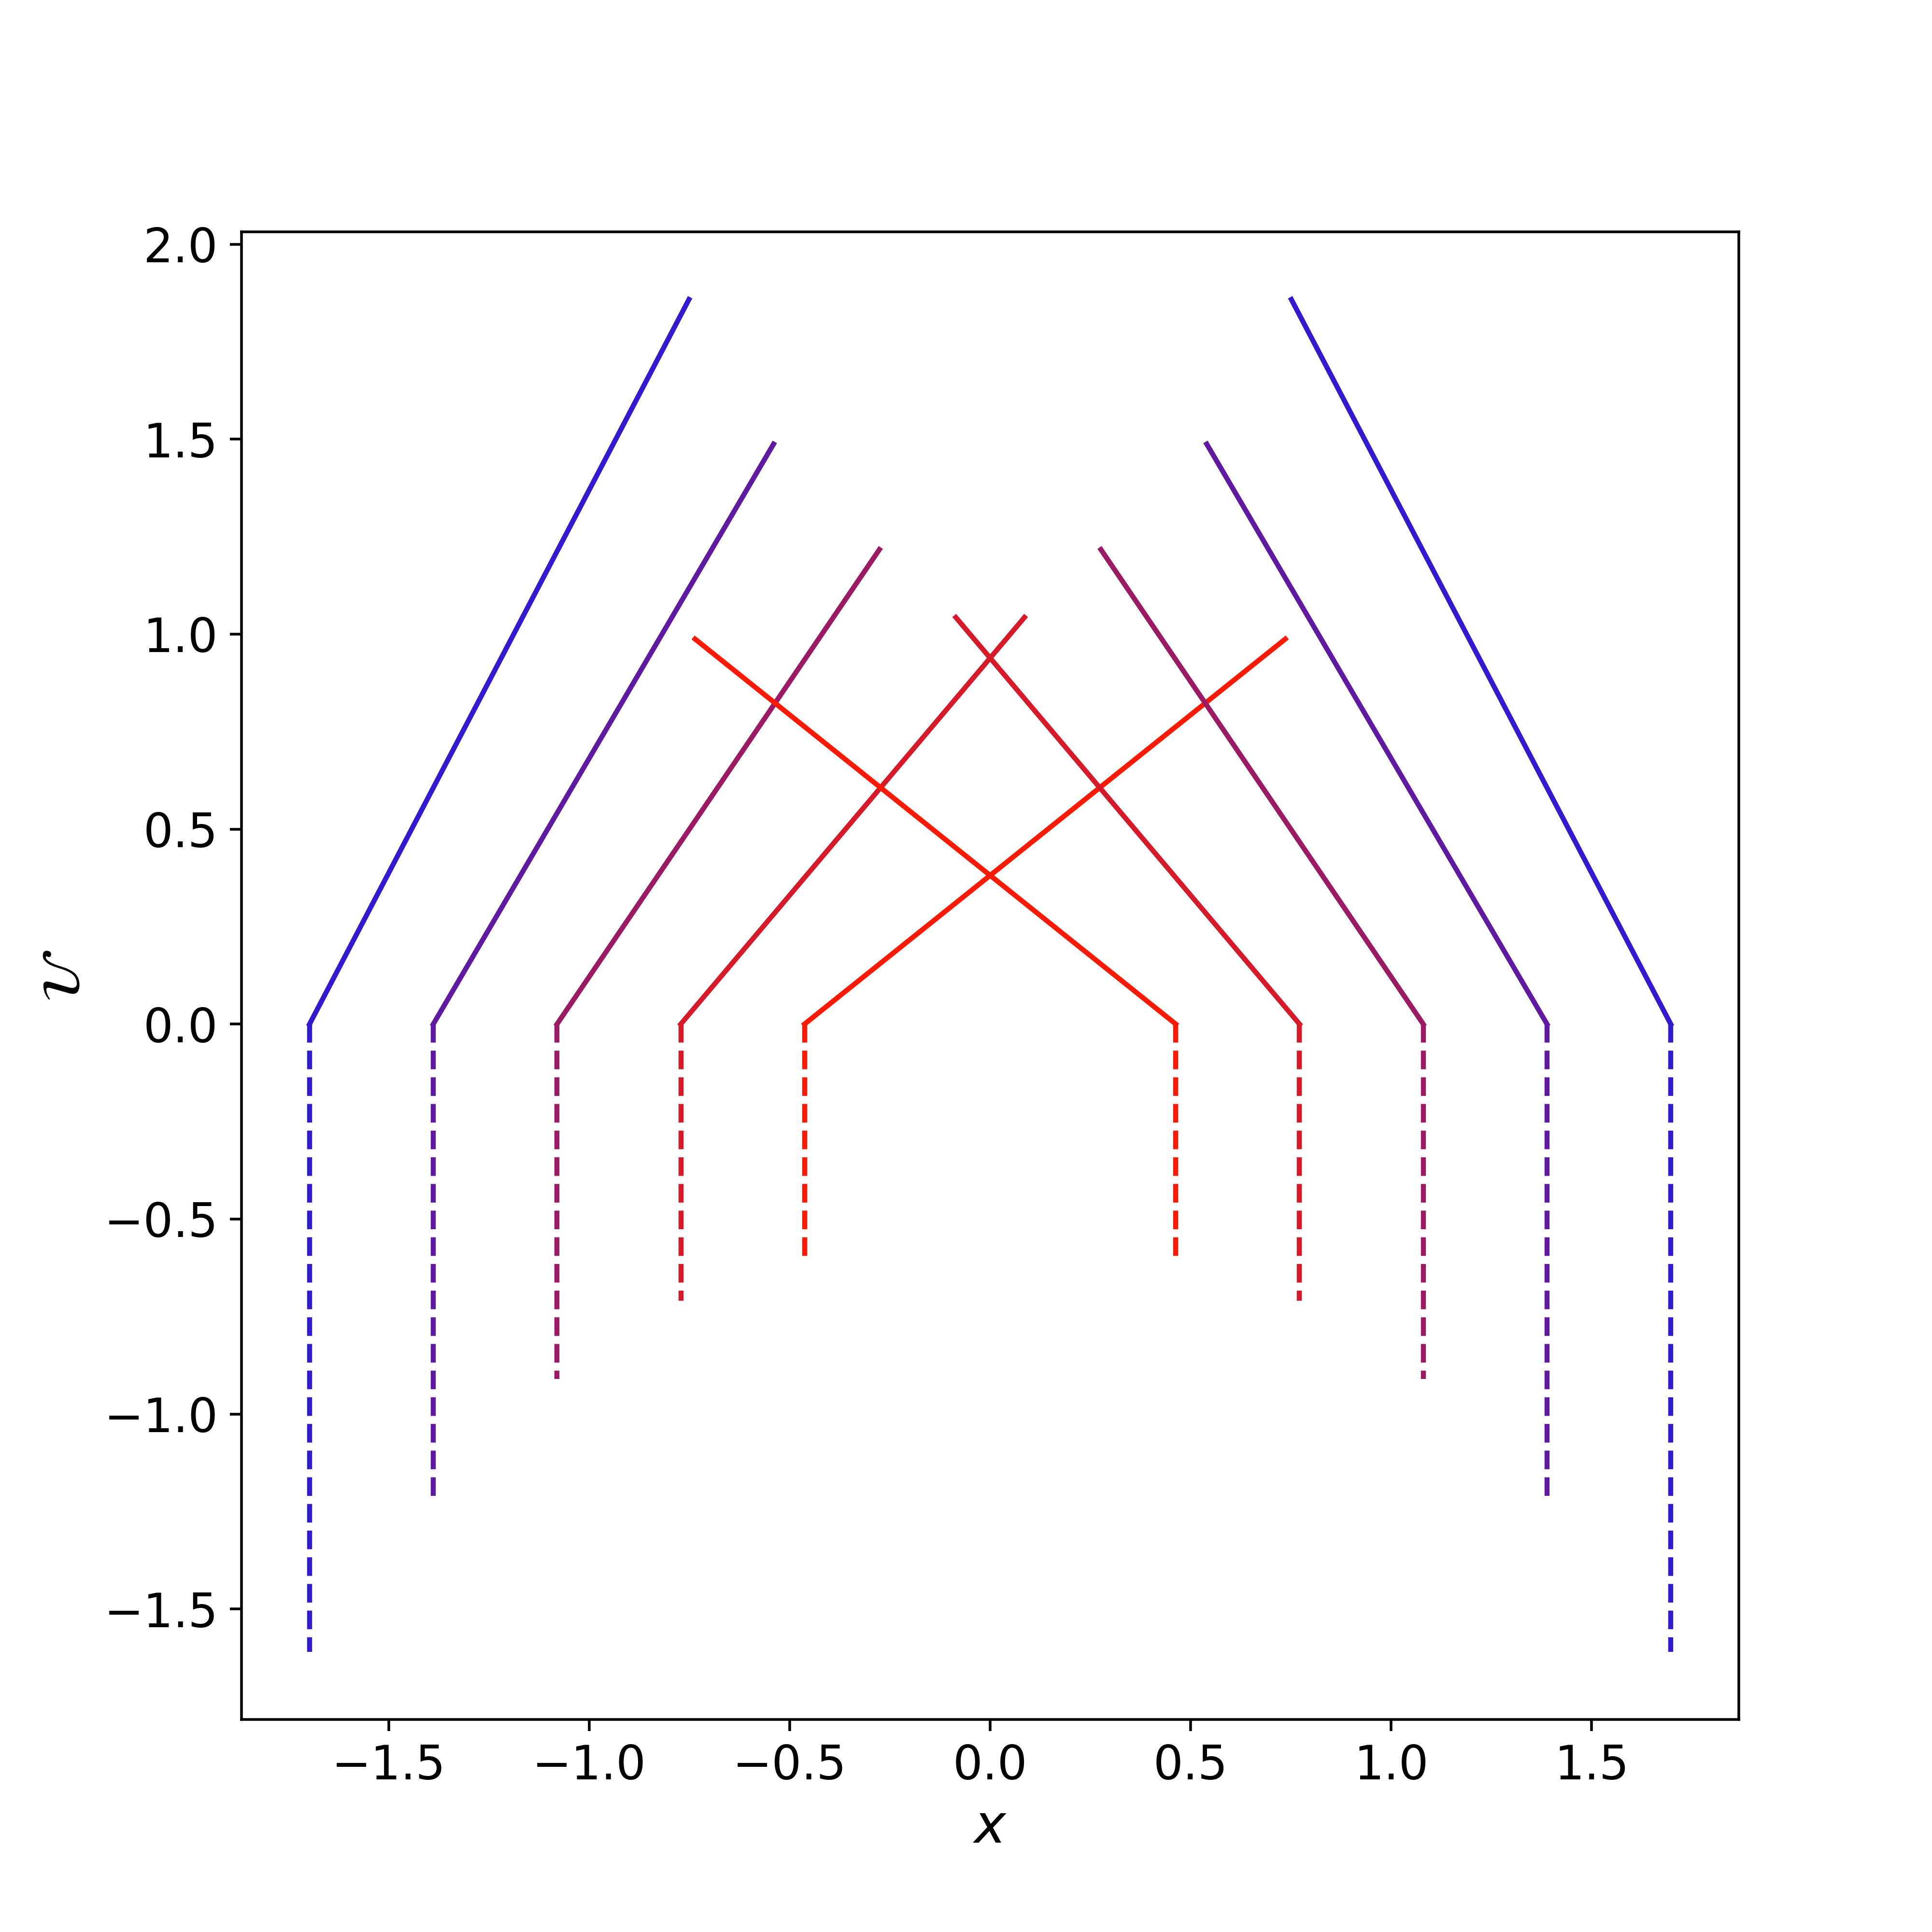
\includegraphics[width=.95\textwidth, clip]{../img/kap02/HT_y-0__xU_mu1_lmb-1,5.png}};
            \filldraw[white] (0.29,3.1) circle (4pt);
            \node[text width=7pt] at (0.29,3.1) {\scriptsize{$\matu$}};
            \filldraw[white] (3.25,0.28) circle (4pt);
            \node[text width=7pt] at (3.25,0.28) {\scriptsize{$x$}};
        \end{tikzpicture}
        \caption{$\Lambda = -1,5$}
    \end{subfigure}
    \caption{Geodetický pohyb nulové částice ($\dot \matu^-=1$, $\dot \matv^-=0$, $\dot \eta^-=0$) v nadploše $y = 0$ v Hottově--Tanakově řešení s parametrem $b_0 = 1$.}
    \label{fig:HottaTanakaNullY0}
\end{figure}

Pro nulové částice nenacházející se na nadploše obsahující osu symetrie dostáváme očekávané strhnutí k
ose symetrie Hottova--Tanakova řešení, k $\eta=0$ (viz obrázek \ref{fig:HottaTanakaNullYsqrt2}). 

\begin{figure}[ht]
    \centering
    \begin{subfigure}[b]{0.45\textwidth}
        \begin{tikzpicture}
            \node[inner sep=0pt, anchor=south west] (ds) at (0,0)
            {\adjincludegraphics[trim={{.08\width} {.1\height} {.12\width} {.15\height}}, width=.95\textwidth, clip]{../img/kap02/HT_y-1__x-y-U_mu1_lmb1.pdf}};
            \filldraw[white] (5,1.2) circle (4pt);
            \node[text width=7pt] at (5, 1.2) {\footnotesize{$\matu$}};
            \filldraw[white] (1.55,1.2) circle (4pt);
            \node[text width=7pt] at (1.55,1.2) {\footnotesize{$x$}};
            \filldraw[white] (0.35,2.85) circle (4pt);
            \node[text width=7pt] at (0.35,2.85) {\footnotesize{$y$}};
        \end{tikzpicture}
        \caption{$\Lambda = 1$}
    \end{subfigure}
    \hfill
    \begin{subfigure}[b]{0.45\textwidth}
        \begin{tikzpicture}
            \node[inner sep=0pt, anchor=south west] (ds) at (0,0)
            {\adjincludegraphics[trim={{.08\width} {.1\height} {.12\width} {.15\height}}, width=.95\textwidth, clip]{../img/kap02/HT_y-1__x-y-U_mu1_lmb-1.pdf}};
            \filldraw[white] (5,1.2) circle (4pt);
            \node[text width=7pt] at (5, 1.2) {\footnotesize{$\matu$}};
            \filldraw[white] (1.55,1.2) circle (4pt);
            \node[text width=7pt] at (1.55,1.2) {\footnotesize{$x$}};
            \filldraw[white] (0.35,2.85) circle (4pt);
            \node[text width=7pt] at (0.35,2.85) {\footnotesize{$y$}};
        \end{tikzpicture}
        \caption{$\Lambda = -1$}
    \end{subfigure}
    \caption{Geodetický pohyb nulových částic ($\dot \matu^-=1$, $\dot \matv^-=0$, $\dot \eta^-=0$) v~nadploše $y = \sqrt{2}$ v Hottově-Tanakově řešení s parametrem $b_0 = 1$.}
    \label{fig:HottaTanakaNullYsqrt2}
\end{figure}

Pro porovnání efektu impulzní vlny na časupodobné testovací částice v konformně plochých souřadnicích byly vykresleny případy geodetického pohybu v prostoročasu bez vlny
a v prostoročasu s impulzní vlnou s parametrem $b_0=3$.

\begin{figure}[ht]
    \centering
    \begin{subfigure}[b]{0.48\textwidth}
        \begin{tikzpicture}
            \node[inner sep=0pt, anchor=south west] (ds) at (0,0)
            {\adjincludegraphics[trim={{.08\width} {.05\height} {.12\width} {.15\height}}, width=.95\textwidth, clip]{../img/kap02/HT1_ring_matter__x-y-U_mu0_lmb1.pdf}};
            \filldraw[white] (0.35,3.46) circle (5pt);
            \node[text width=7pt] at (0.35,3.46) {\footnotesize{$\matu$}};
            \filldraw[white] (5.25,1.05) circle (5pt);
            \node[text width=7pt] at (5.25,1.05) {\footnotesize{$x$}};
            \filldraw[white] (1.75,1.05) circle (5pt);
            \node[text width=7pt] at (1.75,1.05) {\footnotesize{$y$}};
        \end{tikzpicture}
        \caption{de Sitter $(\Lambda = 1)$}
    \end{subfigure}
    \hfill
    \begin{subfigure}[b]{0.48\textwidth}
        \begin{tikzpicture}
            \node[inner sep=0pt, anchor=south west] (ds) at (0,0)
            {\adjincludegraphics[trim={{.08\width} {.05\height} {.12\width} {.15\height}}, width=.95\textwidth, clip]{../img/kap02/HT2_ring_matter__x-y-U_mu3_lmb1.pdf}};
            \filldraw[white] (0.35,3.46) circle (5pt);
            \node[text width=7pt] at (0.35,3.46) {\footnotesize{$\matu$}};
            \filldraw[white] (5.25,1.05) circle (5pt);
            \node[text width=7pt] at (5.25,1.05) {\footnotesize{$x$}};
            \filldraw[white] (1.75,1.05) circle (5pt);
            \node[text width=7pt] at (1.75,1.05) {\footnotesize{$y$}};
        \end{tikzpicture}
        \caption{Hotta--Tanaka$(\Lambda = 1)$}
    \end{subfigure}

    \begin{subfigure}[b]{0.48\textwidth}
        \begin{tikzpicture}
            \node[inner sep=0pt, anchor=south west] (ds) at (0,0)
            {\adjincludegraphics[trim={{.08\width} {.05\height} {.12\width} {.15\height}}, width=.95\textwidth, clip]{../img/kap02/HT3_ring_matter__x-y-U_mu0_lmb-1.pdf}};
            \filldraw[white] (0.35,3.46) circle (5pt);
            \node[text width=7pt] at (0.35,3.46) {\footnotesize{$\matu$}};
            \filldraw[white] (5.25,1.05) circle (5pt);
            \node[text width=7pt] at (5.25,1.05) {\footnotesize{$x$}};
            \filldraw[white] (1.75,1.05) circle (5pt);
            \node[text width=7pt] at (1.75,1.05) {\footnotesize{$y$}};
        \end{tikzpicture}
        \caption{Anti--de Sitter $(\Lambda = -1)$}
    \end{subfigure}
    \hfill
    \begin{subfigure}[b]{0.48\textwidth}
        \begin{tikzpicture}
            \node[inner sep=0pt, anchor=south west] (ds) at (0,0)
            {\adjincludegraphics[trim={{.08\width} {.05\height} {.12\width} {.15\height}}, width=.95\textwidth, clip]{../img/kap02/HT4_ring_matter__x-y-U_mu3_lmb-1.pdf}};
            \filldraw[white] (0.35,3.46) circle (5pt);
            \node[text width=7pt] at (0.35,3.46) {\footnotesize{$\matu$}};
            \filldraw[white] (5.25,1.05) circle (5pt);
            \node[text width=7pt] at (5.25,1.05) {\footnotesize{$x$}};
            \filldraw[white] (1.75,1.05) circle (5pt);
            \node[text width=7pt] at (1.75,1.05) {\footnotesize{$y$}};
        \end{tikzpicture}
        \caption{Hotta-Tanaka $(\Lambda = -1)$}
    \end{subfigure}
    \caption{Časupodobné geodetiky ($\dot \matu^-=\frac{1}{2N}$, $\dot \matv^-=-\frac{1}{N}$, $\dot \eta^-=0$), kde $N$ je normalizační faktor, v (A)--dS a Hottově--Tanakově řešení s parametrem $b_0 = 3$.}
    \label{fig:HottaTanakaMatter}
\end{figure}

Dále vizualizujeme efekt refrakce geodetik v 5--dimenzionálním formalismu. Nulové geodetiky tvoří generátory (A)--dS hyperboloidu, protože při refrakci nedochází
ke změně kauzálního charakteru, po refrakci zůstává geodetika generátorem hyperboloidu, ale, jak vyplývá z refrakčních rovnic \eqref{eq:refraction_velocity_null_cart}, v jiné nadploše - dochází k refrakci
ve všech směrech, kromě směru normály na vlnoplochu. Případ refrakce nulových částic na de Sitterově prostoročasu je na vizualizován na obrázku \ref{fig:HottaTanaka5D}.

\begin{figure}[ht]
    \centering
    \begin{tikzpicture}
        \node[inner sep=0pt, anchor=south west] (ds) at (0,0)
        {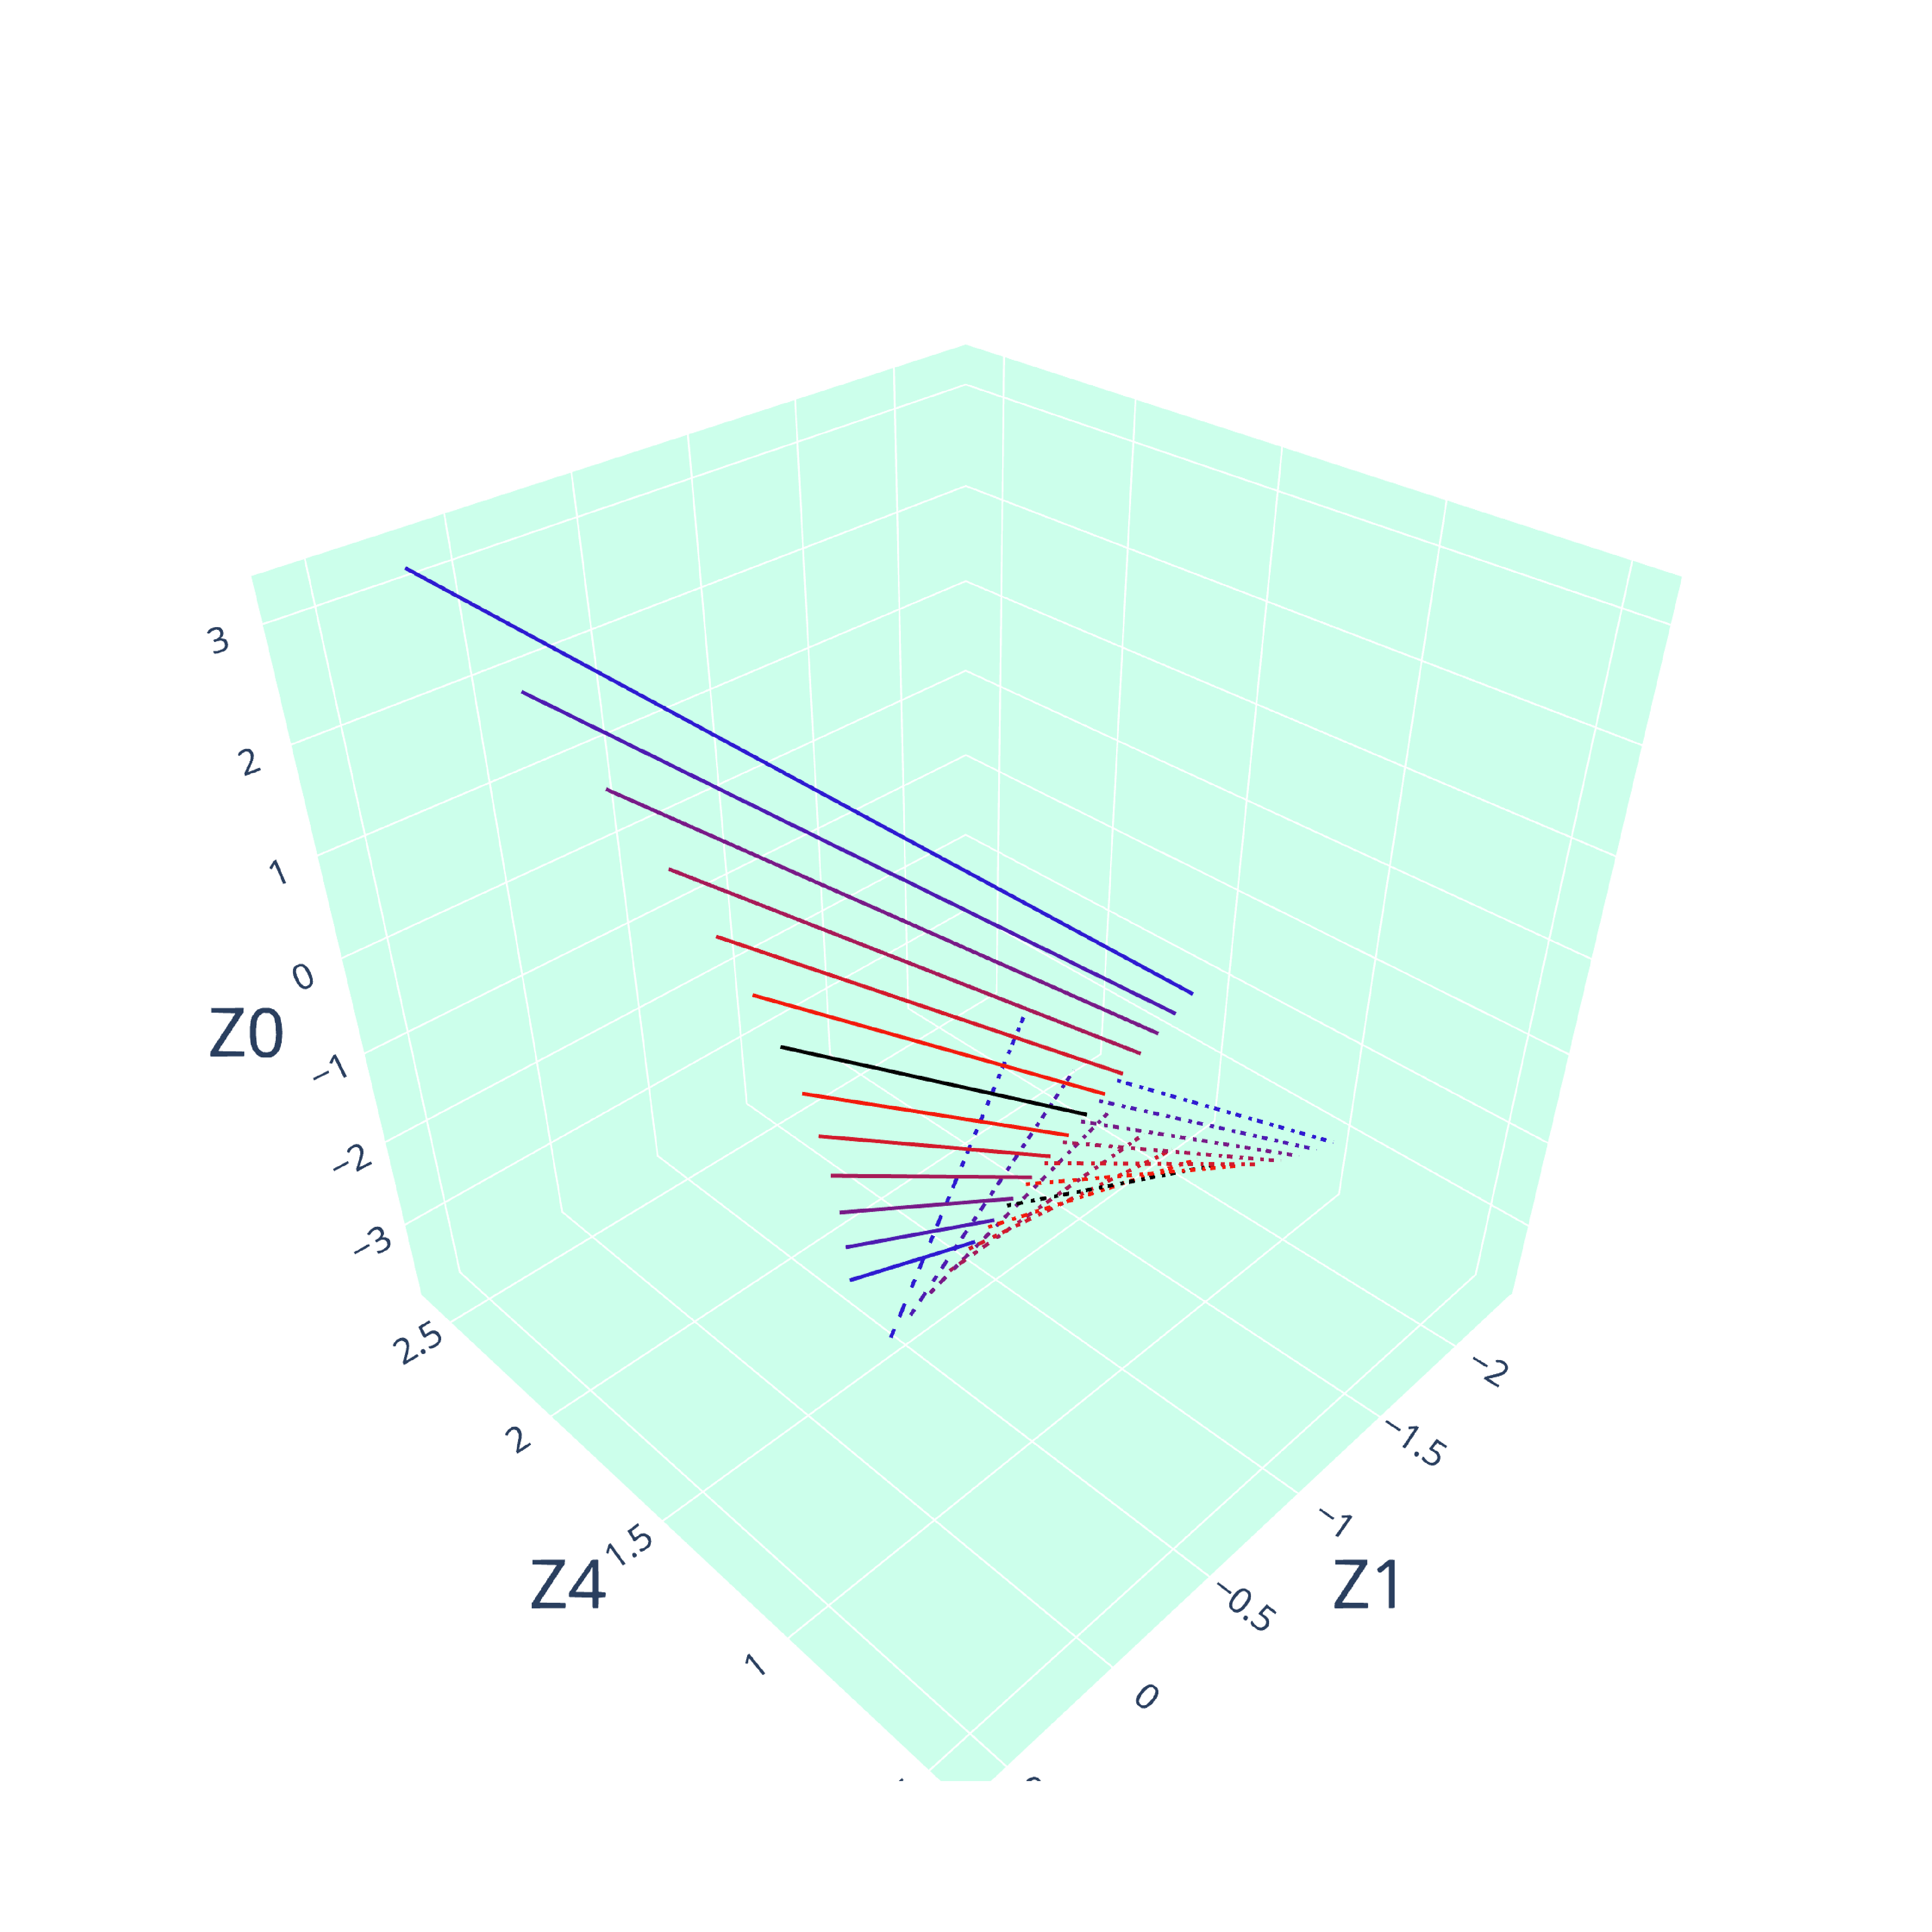
\includegraphics[width=.95\textwidth, clip]{../img/kap02/HT1_x1_null__Z0-Z1-Z4_mu1_lmb1.pdf}};
        \filldraw[white] (1.65,6.35) circle (12pt);
        \node[text width=14pt] at (1.65,6.35) {\normalsize{$Z_0$}};
        \filldraw[white] (4.02,2.33) circle (12pt);
        \node[text width=14pt] at (4.02,2.33) {\normalsize{$Z_4$}};
        \filldraw[white] (9.8,2.4) circle (12pt);
        \node[text width=14pt] at (9.8,2.4) {\normalsize{$Z_1$}};
    \end{tikzpicture}
    \caption{Geodetický pohyb nulové částice ($\dot \matu^-=1$, $\dot \matv^-=0$, $\dot \eta^-=0$) procházející vlnoplochou $\Lambda=1$ Hottova--Tanakova řešení s parametrem $b_0 = 1$ v~$\eta=1,5$ a různých časech (tedy v různých hodnotách souřadnice $\matv$) vyobrazený ve vnoření do $\mathbb{E}^{1,4}$.}
    \label{fig:HottaTanaka5D}
\end{figure}

\cleardoublepage
\chapter{Neexpandující gravitační vlny s gyratonovými členy}
\label{chap:kap03}
Distribuční vyjádření metriky impulzní vlny \eqref{eq:nonexp_distr_metric_omega} není nejobecnější metrikou popisující
impulzní vlny. Lze jí rozšířit o mimodiagonální členy do tvaru
\begin{equation}
    \label{eq:nonexp_gyra_distrib_metric_omega}
    \begin{split}
        \mathrm{d}s^2=&\frac{2\mathrm{d}\eta~\mathrm{d}\bar{\eta} - 2 \mathrm{d}\mathcal{U}~\mathrm{d}\mathcal{V} + 2H(\eta, \bar{\eta}) \delta(\mathcal{U}) 
        ~\mathrm{d}\mathcal{U}^2}{\left[1+\frac{1}{6}\Lambda(\eta \bar{\eta}-\mathcal{U}\mathcal{V})\right]^2} \\
        &+ \frac{2J\left(\eta, \bar{\eta}, \mathcal{U}\right) \mathrm{d}\eta~\mathrm{d}\mathcal{U}
        +2\overline{J}\left(\eta, \bar{\eta}, \mathcal{U}\right) \mathrm{d}\bar{\eta}~\mathrm{d}\mathcal{U}}{\left[1+\frac{1}{6}\Lambda(\eta \bar{\eta}-\mathcal{U}\mathcal{V})\right]^2}.
    \end{split}
\end{equation}
Tvar metriky s mimodiagonálními členy odpovídající gravitační vlně byl uvažován už v Brinkmannově studii \cite{Brinkmann1925} Einsteinových prostoročasů svázaných konformními transformacemi.

Obvyklým postupem je odstranění členů s funkcí $J$ vhodnou souřadnicovou transformací (Brinkmannova forma metriky \emph{pp}-vln \cite{griffiths_podolsky_2009} se také běžně uvádí už bez mimodiagonálních členů), to ale vede k odstranění
možného rotačního charakteru zdroje gravitační vlny, taková transformace pak není globální a dochází ke změně topologických vlastností celého prostoročasu.
Rotující charakter zdrojů byl zkoumán Bonnorem \cite{Bonnor1970} a nezávisle objeven Frolovem a Fursaevem v \cite{Frolov2005_0} a \cite{Frolov2005} Přehled a podrobnější
fyzikální analýzu je možné najít v \cite{Podolsky2014}.
V této kapitole budeme studovat a vizualizovat vliv nediagonálních prvků metriky.

\section{Zobecnění impulzních vln na prostoročasy s~gyratonovými členy}
Konstrukce neexpandujících gracitačních vln s mimodagonálními gyratonovými členy je obdobná konstrukci prostoročasů bez gyratonů z minulé kapitoly, popíšeme ji formalismem spojitých souřadnic
použitým v \cite{Podolsky_2017}, kde jsou také odvozeny refrakční rovnice pro pohyb testovacích částic, pomocí kterých budeme vizualizovat geodetický pohyb procházející impulzní vlnoplochou.

Penroseova "cut and paste"\ konstrukce vede i v případě gyratonových prostoročasů na Penroseovy lepící podmínky ve tvaru \eqref{eq:lepici_podminky}, začneme tedy rovnou zobecněním
spojitého tvaru metriky z předchozí kapitoly.

\subsection{Zobecnění spojitého tvaru metriky}
Tvar spojité metriky pro gyratonové neexpandující impulzní vlny obdržíme zobecněním transformace \eqref{eq:nonexp_cont_full_transform},
do tvaru který nalezli Podolský, Švarc, Sämann a Steinbauer v \cite{Podolsky_2017}
\begin{equation}
    \label{eq:gyraton_cont_transformation}
    \begin{split}
        \matu &= U \\
        \matv &= V + \Theta H + U_{+} H_{,Z} H_{,\bar{Z}} + W \\
        \eta &= \left(Z + U_{+} H_{,\bar{Z}}\right) \exp \left(i F \right),
    \end{split}
\end{equation}

kde opět $H = H(Z, \bar{Z})$, zároveň funkce $W = W(Z, \bar{Z}, U)$ a $F = F(Z, \bar{Z}, U)$ jsou reálné a splňují
\begin{equation}
    \label{eq:podminky_F_a_W}
    \begin{split}
        F_{,U} &= \frac{i\bar{J}}{Z + U_{+}H_{,\bar{Z}}} \exp{\left(-iF\right)}, \\
        W_{,U} &= -J \bar{J}, \\
        W &= 0 \text{ pro } U \leq 0.
    \end{split}
\end{equation}
Zavedením
\begin{equation}
    \zeta \equiv Z + U_{+} H_{,\bar{Z}}
\end{equation}
a prostorového diferenciálu $\underline{\rmd}$ tak, že
\begin{equation}
    \label{eq:spatial_differential_on_functions}
    \begin{split}
        \underline{\rmd}\zeta &\equiv \rmd Z + U_{+}(H_{,\bar{Z}Z}\rmd Z + H_{,\bar{Z}\bar{Z}}\rmd \bar{Z}), \\
        \underline{\rmd}H &\equiv H_{,Z}\rmd Z + H_{,\bar{Z}}\rmd \bar{Z}, \\
        \underline{\rmd}F &\equiv F_{,Z}\rmd Z + F_{,\bar{Z}}\rmd \bar{Z}, \\
        \underline{\rmd}W &\equiv W_{,Z}\rmd Z + W_{,\bar{Z}}\rmd \bar{Z},
    \end{split}
\end{equation}
dosazením \eqref{eq:gyraton_cont_transformation} do \eqref{eq:nonexp_gyra_distrib_metric_omega} a využitím vztahů \eqref{eq:podminky_F_a_W},
\eqref{eq:spatial_differential_on_functions} a multiplikativních pravidel z nelineární teorie distribucí,
\begin{equation}
    \label{eq:pravidla_distribuce}
    \Theta^2 = \Theta, ~~~~~~ \Theta U_{+} = U_{+},
\end{equation}
dostaneme metriku ve spojitém tvaru
\begin{equation}
    \label{eq:spojita_gyratonova_metrika}
    \rmd s^2 = \frac{2 \left|\underline{\rmd} \zeta + i \zeta \underline{\rmd}F\right|^2 + 2 \left[i \Theta\left(\zeta H_{,Z} - \bar{\zeta} H_{,\bar{Z}}\right) \underline{\rmd}F - \underline{\rmd}W\right] \rmd U - 2\rmd U \rmd V}{\left[1+\frac{1}{6}\Lambda\left(Z \bar{Z} - UV - U_{+}G\right)\right]^2},
\end{equation}
kde byla zavedena funkce
\begin{equation}
    G \left( Z, \bar{Z}, U \right) = H - Z H_{,Z} - \bar{Z} H_{,\bar{Z}} + W.
\end{equation}

Oproti minulé kapitole se ve funkci $G$ vyskytuje člen $W$. Aplikací transformace \eqref{eq:gyraton_cont_transformation}
na konformní faktor $\Omega = 1 + \frac{1}{6} \Lambda (\eta \bar{\eta} - \matu \matv)$ dostáváme po použití pravidel násobení distribucí v nelineární teorii \eqref{eq:pravidla_distribuce} tvar
\begin{equation}
    \Omega = 1 + \frac{1}{6} \Lambda \left(Z \bar{Z} - UV - U_+ (H - Z H_{,Z} \bar{Z} H_{,\bar{Z}}) - UW \right).
\end{equation}
V případě že $W = 0$ pro $U \leq 0$, platí $UW = U_+ W$. To je ale splněno v \eqref{eq:podminky_F_a_W} a tvar funkce $G$ je tedy ospravedlněn.

Volba $J=0$ dovoluje řešení $F = W = 0$, přičemž se metrika \eqref{eq:spojita_gyratonova_metrika} redukuje na \eqref{eq:nonexp_continuous_metric}.
Metrika \eqref{eq:spojita_gyratonova_metrika} je spojitá v případě, že $\underline{\rmd}F$ a $\underline{\rmd}W$ jsou funkce spojité v $U$ a $\underline{\rmd}F$
jde v $U=0$ k nule. V tomto případě je metrika lokálně lipschitzovská a lze využít formalismu Filippovových řešení, jako v předchozí kapitole.


\subsection{Frolovův--Fursaevův gyraton}
Dále budeme uvažovat konkrétní realizaci gyratonového prostoročasu, tedy metriku \eqref{eq:nonexp_gyra_distrib_metric_omega} s volbou
\begin{equation}
    J(\eta , \matu) = \frac{\chi}{2 i \eta} \Theta( \matu ),~~~ \Lambda = 0,
\end{equation}
kde $\chi$ je konstantní. Rovnice \eqref{eq:podminky_F_a_W} lze zintegrovat do tvaru
\begin{equation}
    \label{eq:zintegrovane1}
    \begin{split}
        F &= \frac{\chi}{2(Z H_{,Z}-\bar{Z}H_{,\bar{Z}})} \log \frac{Z\bar{Z}+U_{+}\bar{Z}H_{,\bar{Z}}}{Z\bar{Z}+U_{+}ZH_{,Z}}, \\
        W &= \frac{\chi}{2}F,
    \end{split}
\end{equation}
kde přirozeně uvažujeme hlavní větev logaritmu, aby se zachovala rovnost $\eta = Z$ pro $U \leq 0$.

V případě že $Z H_{,Z} - \bar{Z}H_{,\bar{Z}}=0 \iff \log \frac{Z \bar{Z} + U_{+}\bar{Z}H_{,\bar{Z}}}{Z\bar{Z}+U_{+}ZH_{,Z}}=0$
není tvar \eqref{eq:zintegrovane1} platný. Diferenciální operátor působící na funkci $H$ v levé části ekvivalence
lze (díky $Z = \frac{1}{\sqrt{2}} \rho \exp(i \phi)$) zapsat jako $Z \partial_Z - \bar{Z}\partial_{\bar{Z}} = - i \partial_\phi$,
jedná se tedy o generátor rotace kolem osy $Z = 0$. Tento případ tedy nastává ve všech axiálně symetrických prostoročasech, kde
funkce $H$ závisí pouze na $\rho^2 = 2 Z \bar{Z}$, včetně Aichelburg--Sexlova řešení
$H = b_0 \log(2\eta \bar{\eta}) = b_0 \log (2Z \bar{Z})$, kterým se budeme dále zabývat.
Funkce $F$ a $W$ lze v takovém případě volit ve tvaru
\begin{equation}
    \label{eq:zintegrovane2}
    \begin{split}
        F &= -\frac{\chi}{2} \frac{U_{+}}{Z \bar{Z} + b_0 U_{+}}, \\
        W &= \frac{\chi}{2}F,
    \end{split}
\end{equation}
spojitá metrika nabývá tvaru z třídy Frolovových--Fursaevových gyratonů \cite{Frolov2005} 
\begin{equation}
    \begin{split}
    \rmd s^2 = &2 \left| \rmd Z + U_{+} \left(i \frac{\chi}{2}\frac{\bar{Z}\rmd Z + Z \rmd \bar{Z}}{\bar{Z}\left(Z \bar{Z} + b_0 U_{+}\right)} - b_0 \frac{d\bar{Z}}{\bar{Z}^2}\right) \right|^2 \\
    &- \frac{\chi^2}{2}U_{+}\frac{\bar{Z} \rmd Z \rmd U + Z \rmd \bar{Z} \rmd U}{\left(Z \bar{Z} + b_0 U_{+}\right)^2} - 2 \rmd U \rmd V
    \end{split}
\end{equation}
reprezentujících zobecnění
originální Aichelburg--Sexlovy metriky \cite{Aichelburg_1971} na impulzní vlnu generovanou částicí s
nenulovým vnitřním momentem hybnosti, přičemž $\chi \Theta(\matu)$ odpovídá hustotě momentu hybnosti gyratonu \cite{Podolsky2014}.
Při absenci gyratonu ($\chi=0$) se metrika redukuje na standardní Aichelburg--Sexlovo řešení.

Díky tomu, že pracujeme v konformně plochých souřadnicích, nejsou výše uvedené závěry závislé na kosmologické konstantě.
Za funkci $H$ pak můžeme uvažovat například Hottovo--Tanakovo řešení \eqref{eq:Hotta_Tanaka_H_conf_flat_coords}. Pro toto řešení nebudeme explicitně odvozovat
spojitý tvar metriky, později ale využijeme formalismus refrakčních rovnic pro vykreslení geodetického pohybu gyratonového zdroje na (anti-)de Sitterově prostoročasu
s výše uvedenou funkcí $J$ a funkcí $H$ odpovídající právě Hottově--Tanakově řešení. Zmíníme ale, že ekvivalence znemožňující integraci funkcí $F$ a $W$ do tvaru
\eqref{eq:zintegrovane1} neplatí ani v tomto případě, jedná se také o axiálně symetrické řešení.


\section{Refrakční rovnice pro geodetiky v impulzních gyratonových prostoročasech}
Stejně jako v případě bez gyratonových členů v předchozí kapitole, i zde k vizualizaci geodetik využijeme refrakčních rovnic,
které byly pro impulzní neexpandující gyratonové prostoročasy s funkcemi $F$ a $W$ ve tvaru
\eqref{eq:zintegrovane1}, resp. \eqref{eq:zintegrovane2}, odvozeny z limity spojitých souřadnic \eqref{eq:spojita_gyratonova_metrika}
v $\matu = 0$ v článku \cite{Podolsky_2017}.
Napojovací podmínky prostorových poloh jsou v tomto případě ve tvaru
\begin{equation}
    \label{eq:refrakcni_rovnice_gyra_polohy}
    \begin{split}
        \matu_{\rmi}^{+} &= \matu_{\rmi}^{-}, \\
        \matv_{\rmi}^{+} &= \matv_{\rmi}^{-} + H_{\rmi}, \\
        \eta_{\rmi}^{+} &= \eta_{\rmi}^{-},
    \end{split}
\end{equation}
což přesně odpovídá Penroseovým napojovacím podmínkám \eqref{eq:lepici_podminky},
jejichž tvar nezávisí na přítomnosti gyratonových členů. Co se bude lišit od
výsledků popsaných v minulé kapitole jsou refrakční rovnice pro složky rychlosti,
\begin{equation}
    \label{eq:refrakcni_rovnice_gyra_rychlosti}
    \begin{split}
        \dot{\matu}_{\rmi}^{+} &= \dot{\matu}_{\rmi}^{-}, \\
        \dot{\matv}_{\rmi}^{+} &= \dot{\matv}_{\rmi}^{-} + H_{\rmi, Z} \dot{\eta}_{\rmi}^{-} + H_{\rmi, \bar{Z}} \dot{\bar{\eta}}_{\rmi}^{-} + \left(H_{\rmi, Z} H_{\rmi, \bar{Z}} - \frac{\chi^2}{4 \eta_{\rmi}^{-} \bar{\eta}_{\rmi}^{-}}\right) \dot{\matu}_{\rmi}^{-} \\
        \dot{\eta}_{\rmi}^{+} &= \dot{\eta}_{\rmi}^{-} + \left(H_{\rmi, \bar{Z}} - \frac{i \chi}{2 \bar{\eta}_{\rmi}^{-}}\right) \dot{\matu}_{\rmi}^{-},
    \end{split} 
\end{equation}
kde gyratonové členy s $\chi$ přispívají ke skoku ve složkách $\dot{\matv}_{\rmi}$ a $\dot{\eta}_{\rmi}$ členy
\begin{equation}
    \Delta \dot{\matv}_{\rmi} = -\frac{\chi^2}{4 \eta_{\rmi}^{-} \bar{\eta}_{\rmi}^{-}} \dot{\matu}_{\rmi}^{-}, ~~~~~~ \Delta \dot{\eta}_{\rmi} = -\frac{i \chi}{2 \bar{\eta}_{\rmi}^{-}} \dot{\matu}_{\rmi}^{-}.
\end{equation}
Tyto skoky navíc se díky $C^1-$regularitě geodetik a spojitosti metriky kompenzují, neboť normalizace čtyřrychlosti musí být zachována, a platí
\begin{equation}
    \Delta \dot{\eta}_{\rmi} \Delta \dot{\bar{\eta}}_{\rmi} = - \dot{\matu}_{\rmi} \Delta \dot{\matv}_{\rmi}.
\end{equation}
Tyto skoky pro $\eta_{\rmi}^{-} \to 0$ rostou nad všechny meze, toto chování ale očekáváme -- v $\eta_{\rmi} = 0$ se nachází bodový zdroj.
Pro $\chi \to 0$ se tyto rovnice redukují na rovnice \eqref{eq:refraction_nonexpanding_velocities} z minulé kapitoly.

Obdobně jako v předchozí kapitole, refrakční rovnice \eqref{eq:refrakcni_rovnice_gyra_rychlosti} můžeme také zapsat v reálných
polárních souřdnicích jako
\begin{equation}
    \begin{split}
    \dot{\matv}_{\rmi}^{+} &= \dot{\matv}_{\rmi}^{-} + \halfsqrt \left(e^{i \varphi_{\rmi}^{-}} H_{\rmi, Z} + e^{-i \varphi_{\rmi}^{-}} H_{\rmi, \bar{Z}}\right) \dot{\rho}_{\rmi}^{-} +
    \frac{i}{\sqrt{2}} \left( e^{i \varphi_{\rmi}^{-}} H_{\rmi, Z} - e^{-i \varphi_{\rmi}^{-}} H_{\rmi, \bar{Z}} \right) \rho_{\rmi}^{-} \dot{\varphi}_{\rmi}^{-} \\
    &~~~+ \left(H_{\rmi, Z} H_{\rmi, \bar{Z}} - \frac{\chi^2}{2(\rho_{\rmi}^{-})^2}\right)\dot{\matu}_{\rmi}^{-}, \\
    \dot{\rho}_{\rmi}^{+} &= \dot{\rho}_{\rmi}^{-} + \halfsqrt \left(e^{-i \varphi_{\rmi}^{-}} H_{\rmi, \bar{Z}} + e^{i \varphi_{\rmi}^{-}} H_{\rmi, Z} \right), \\
    \dot{\varphi}_{\rmi}^{+} &= \dot{\varphi}_{\rmi}^{-} + \left[ \frac{i}{\sqrt{2} \rho_{\rmi}^{-}} \left(e^{i \varphi_{\rmi}^{-}} H_{\rmi, Z} - e^{-i \varphi_{\rmi}^{-}} H_{\rmi, \bar{Z}} \right) - \frac{\chi}{(\rho_{\rmi}^{-})^2}\right] \dot{\matu}_{\rmi}^{-}.
    \end{split}
\end{equation}
Tento tvar potvrzuje interpretaci gyratonových členů jako interního momentu hybnosti částice generující impulz -- 
přítomnost gyraonických členů nemá vliv na radiální složku $\dot{\rho}$, přispívá ale k další změně v
axiální složce $\dot{\varphi_{\rmi}}$ členem $\frac{\chi}{(\rho_{\rmi})^2}$.

\section{Vizualizace geodetik v neexpandujících impulzních gyratonových prostoročasech}
V této části budeme explicitně analyzovat geodetický pohyb v prostoročasech s gyratonovými zdroji, generujícími impulzní vlny.
\subsection{Geodetický pohyb ve Frolovově--Fursaevově gyratonovém řešení}

Stejně jako v minulé kapitole využijeme refrakční rovnice \eqref{eq:refrakcni_rovnice_gyra_polohy}, \eqref{eq:refrakcni_rovnice_gyra_rychlosti}
k vizualizaci interakce impulzního Frolova--Fursaevova gyratonu s geodetikami na prostoročasech tvořících pozadí impulzní vlny.
V případě gyratonu je pozadí odlišné, pro $\Lambda = 0$ je prostoročas $\mathcal{M}^{-}$ (před impulzní vlnou) Minkowského prostoročas,
za impulzní vlnou je ale pozadí $\mathcal{M}^+$ popsáno metrikou
\begin{equation}
    \rmd s^2 = - 2 \rmd \matu ~ \rmd \matv + 2 \rmd \eta ~ \rmd \bar{\eta} + i \chi \rmd \matu \left(\frac{\rmd \bar{\eta}}{\bar{\eta}} - \frac{\rmd \eta}{\eta}\right),
\end{equation}
jediné nenulové Christoffelovy symboly jsou
\begin{equation}
    \Gamma^{\matv}_{\eta \eta} = - \frac{i \chi}{2 \eta^2} ~~~~~ \Gamma^{\matv}_{\bar{\eta}\bar{\eta}} = \frac{i \chi}{2 \bar{\eta}^2}.
\end{equation}

Rotující charakter zdroje je také dobře vidět z metriky za impulzní vlnou při parametrizaci reálnými souřadnicemi $(x, y)$ \eqref{eq:complex_coordinates},
ve kterých metrika nabývá tvaru
\begin{equation}
    \label{eq:gyra_plus_uv_metric}
    \rmd s^2 = -2 \rmd \matu ~ \rmd \matv + \rmd x^2 + \rmd y^2 + \frac{2 \chi \rmd \matu (x~\rmd y - y~\rmd x)}{x^2 + y^2}.
\end{equation}
Transformací do standardních polárních souřadnic $x = r \sin{\varphi}, y = r \cos{\varphi}$ přechází metrika \eqref{eq:gyra_plus_uv_metric} do tvaru
\begin{equation}
    \rmd s^2 = \rmd r^2 + r^2 \rmd \varphi^2 - 2 \rmd \matu (\rmd \matv + \chi \rmd \varphi).
\end{equation}
Prostoročas za vlnou se tak netriviálně liší od maximálně symetrického pozadí (nejedná se ani o statické řešení) a zvolený přístup
numerické integrace rovnice geodetiky zde dostává plný význam.

Na následujících vizualizacích je pro různé hodnoty parametru $\chi$ znázorněno chování nejprve nulových a následně časupodobných geodetik procházejících impulzní plochou v
axiálně symetrickém uspořádání kolem gyratonového zdroje na nadploše $\matu = 0, \matv=0$ v různé vzdálenosti $\rho$ od osy symetrie.

Na obrázku \ref{fig:gyra_flat_null_b1_chi1_2} jsou pro hodnoty $\chi = \pi, 2\pi$ vizualizovány nulové geodetiky procházející nadplochou $\matu = 0$ s
čtyřrychlostí $\dot{\matu} = 1, \dot{\matv} = 0, \dot{\eta} = 0$, oproti negyratonovému řešení, vizualizovanému v předchozí kapitole, dochází
nejen ke strhnutí geodetik k ose symetrie, ale i k vychýlení vlivem rotačního charakteru zdroje. V této vizualizaci se
přítomnost gyratonu projevuje pouze refrakcí na impulzní nadploše -- jediné nenulové Christoffelovy symboly vstupují do geodetické rovnice pro $\matv$.
S~rostoucím parametrem $\chi$ je strhávání silnější.
\begin{figure}[H]
    \centering
    \begin{subfigure}[b]{0.48\textwidth}
        \begin{tikzpicture}
            \node[inner sep=0pt, anchor=south west] (ds) at (0,0)
            {\adjincludegraphics[trim={{.17\width} {.2\height} {.17\width} {.22\height}}, width=1\textwidth, clip]{../img/kap03/flat_gyraton/null/null_gyraton_ring__r_2__mu_1__chi_1pi_uxy.pdf}};
            \filldraw[white] (0.45,2.8) circle (5pt);
            \node[text width=7pt] at (0.45,2.8) {\footnotesize{$\matu$}};
            \filldraw[white] (2,0.55) circle (6pt);
            \node[text width=7pt] at (2,0.55) {\footnotesize{$y$}};
            \filldraw[white] (5.68,0.88) circle (6pt);
            \node[text width=7pt] at (5.68,0.88) {\footnotesize{$x$}};
            \filldraw[white] (0.82,1.13) circle (4pt);
        \end{tikzpicture}
         \caption{$b_0=1, \chi=\pi, \rho=\sqrt{2}$} 
    \end{subfigure}
    \begin{subfigure}[b]{0.48\textwidth}
        \begin{tikzpicture}
            \node[inner sep=0pt, anchor=south west] (ds) at (0,0)
            {\adjincludegraphics[trim={{.17\width} {.2\height} {.17\width} {.22\height}}, width=1\textwidth, clip]{../img/kap03/flat_gyraton/null/null_gyraton_ring__r_3__mu_1__chi_1pi_uxy.pdf}};
            \filldraw[white] (0.45,2.8) circle (5pt);
            \node[text width=7pt] at (0.45,2.8) {\footnotesize{$\matu$}};
            \filldraw[white] (2,0.55) circle (6pt);
            \node[text width=7pt] at (2,0.55) {\footnotesize{$y$}};
            \filldraw[white] (5.68,0.88) circle (6pt);
            \node[text width=7pt] at (5.68,0.88) {\footnotesize{$x$}};
        \end{tikzpicture}
         \caption{$b_0=1, \chi=\pi, \rho=\frac{3}{\sqrt{2}}$} 
    \end{subfigure}
    \hfill
    \begin{subfigure}[b]{0.48\textwidth}
        \begin{tikzpicture}
            \node[inner sep=0pt, anchor=south west] (ds) at (0,0)
            {\adjincludegraphics[trim={{.17\width} {.2\height} {.17\width} {.22\height}},width=1\textwidth, clip]{../img/kap03/flat_gyraton/null/null_gyraton_ring__r_2__mu_1__chi_2pi_uxy.pdf}};
            \filldraw[white] (0.45,2.8) circle (5pt);
            \node[text width=7pt] at (0.45,2.8) {\footnotesize{$\matu$}};
            \filldraw[white] (2,0.55) circle (6pt);
            \node[text width=7pt] at (2,0.55) {\footnotesize{$y$}};
            \filldraw[white] (5.68,0.88) circle (6pt);
            \node[text width=7pt] at (5.68,0.88) {\footnotesize{$x$}};
        \end{tikzpicture}
         \caption{$b_0=1, \chi=2\pi, \rho=\sqrt{2}$} 
    \end{subfigure}
    \begin{subfigure}[b]{0.48\textwidth}
        \begin{tikzpicture}
            \node[inner sep=0pt, anchor=south west] (ds) at (0,0)
            {\adjincludegraphics[trim={{.17\width} {.2\height} {.17\width} {.22\height}}, width=1\textwidth, clip]{../img/kap03/flat_gyraton/null/null_gyraton_ring__r_3__mu_1__chi_2pi_uxy.pdf}};
            \filldraw[white] (0.45,2.8) circle (5pt);
            \node[text width=7pt] at (0.45,2.8) {\footnotesize{$\matu$}};
            \filldraw[white] (2,0.55) circle (6pt);
            \node[text width=7pt] at (2,0.55) {\footnotesize{$y$}};
            \filldraw[white] (5.68,0.88) circle (6pt);
            \node[text width=7pt] at (5.68,0.88) {\footnotesize{$x$}};
        \end{tikzpicture}
         \caption{$b_0=1, \chi=2\pi, \rho=\frac{3}{\sqrt{2}}$} 
    \end{subfigure}
    \caption{Nulové geodetiky procházející impulzní plochou Frolova--Fursaevova gyratonu, vykreslené souřadnice $\matu, x, y$}
    \label{fig:gyra_flat_null_b1_chi1_2}
\end{figure}

\begin{figure}[H]
    \centering
    \begin{subfigure}[b]{0.48\textwidth}
        \begin{tikzpicture}
            \node[inner sep=0pt, anchor=south west] (ds) at (0,0)
            {\adjincludegraphics[trim={{.17\width} {.2\height} {.17\width} {.22\height}}, width=1\textwidth, clip]{../img/kap03/flat_gyraton/null/null_gyraton_ring__r_1__mu_1__chi_2pi_vxy.pdf}};
            \filldraw[white] (0.45,2.8) circle (5pt);
            \node[text width=7pt] at (0.45,2.8) {\footnotesize{$\matv$}};
            \filldraw[white] (2,0.55) circle (6pt);
            \node[text width=7pt] at (2,0.55) {\footnotesize{$y$}};
            \filldraw[white] (5.68,0.88) circle (6pt);
            \node[text width=7pt] at (5.68,0.88) {\footnotesize{$x$}};
        \end{tikzpicture}
        \caption{$b_0=1, \chi=2\pi, \rho=1$}
    \end{subfigure}
    \begin{subfigure}[b]{0.48\textwidth}
        \begin{tikzpicture}
            \node[inner sep=0pt, anchor=south west] (ds) at (0,0)
            {\adjincludegraphics[trim={{.17\width} {.2\height} {.17\width} {.22\height}}, width=1\textwidth, clip]{../img/kap03/flat_gyraton/null/null_gyraton_ring__r_2__mu_1__chi_2pi_vxy.pdf}};
            \filldraw[white] (0.45,2.8) circle (5pt);
            \node[text width=7pt] at (0.45,2.8) {\footnotesize{$\matv$}};
            \filldraw[white] (2,0.55) circle (6pt);
            \node[text width=7pt] at (2,0.55) {\footnotesize{$y$}};
            \filldraw[white] (5.68,0.88) circle (6pt);
            \node[text width=7pt] at (5.68,0.88) {\footnotesize{$x$}};
        \end{tikzpicture}
        \caption{$b_0=1, \chi=2\pi, \rho=\sqrt{2}$} 
    \end{subfigure}
    \caption{Nulové geodetiky po průchodu impulzní plochou Frolova--Fursaevova gyratonu, vykreslené souřadnice $\matv, x, y$}
    \label{fig:gyra_flat_null_b1_chi1_2_vxy}
\end{figure}

Vliv gyratonového charakteru prostoročasu za impulzní plochou je vidět při vizualizaci souřadnice $\matv$ (viz obrázek \ref{fig:gyra_flat_null_b1_chi1_2_vxy}),
při refrakci ve vizualizovaném případě kladná složka $\dot{\matv}$ přechází v zápornou, vlivem gyratonu je ale vynucováno kladné zrychlení a
geodetika se ve směru $\matv$ obrací.

Na obrázku \ref{fig:gyra_skewed_flat_null_b1_chi2} pak vidíme nulové geodetiky procházející impulzní nadplochou
s čtyřrychlostí $\dot{\matu} = 1, \dot{\matv} = 1, \dot{\eta} = 1$, před průchodem $\matu=0$ se v Minkowského části
prostoročasu jednotlivé geodetiky pohybují na nadploše $t, x$.

\begin{figure}[H]
    \centering
    \begin{subfigure}[b]{1\textwidth}
        \begin{subfigure}[b]{0.48\textwidth}
            \begin{tikzpicture}
                \node[inner sep=0pt, anchor=south west] (ds) at (0,0)
                {\adjincludegraphics[trim={{.14\width} {.15\height} {.15\width} {.22\height}}, width=1\textwidth, clip]{../img/kap03/flat_gyraton/null/null_skewed_gyraton_ring__r_1__mu_1__chi_2pi_uxy.pdf}};
                \filldraw[white] (0.39,2.91) circle (5pt);
                \node[text width=7pt] at (0.39,2.91) {\footnotesize{$\matu$}};
                \filldraw[white] (2.2,0.4) circle (6pt);
                \node[text width=7pt] at (2.2,0.4) {\footnotesize{$x$}};
                \filldraw[white] (5.87,1.14) circle (6pt);
                \node[text width=7pt] at (5.87,1.14) {\footnotesize{$y$}};
            \end{tikzpicture}
        \end{subfigure}
        \hfill
        \begin{subfigure}[b]{0.48\textwidth}
            \begin{tikzpicture}
                \node[inner sep=0pt, anchor=south west] (ds) at (0,0)
                {\adjincludegraphics[trim={{.12\width} {.1\height} {.15\width} {.18\height}}, width=1\textwidth, clip]{../img/kap03/flat_gyraton/null/null_skewed_top_gyraton_ring__r_1__mu_1__chi_2pi_uxy.pdf}};
                \filldraw[white] (0.39,3.4) circle (5pt);
                \node[text width=7pt] at (0.39,3.4) {\footnotesize{$\matu$}};
                \filldraw[white] (2,1.4) circle (6pt);
                \node[text width=7pt] at (2,1.4) {\footnotesize{$x$}};
                \filldraw[white] (5.34,1.32) circle (6pt);
                \node[text width=7pt] at (5.34,1.32) {\footnotesize{$y$}};
            \end{tikzpicture}
        \end{subfigure}
        \caption{$b_0=1, \chi=2\pi, \rho=1$, vykreslené souřadnice $\matu, x, y$} 
    \end{subfigure}
    \hfill
    \begin{subfigure}[b]{1\textwidth}
        \begin{subfigure}[b]{0.48\textwidth}
            \begin{tikzpicture}
                \node[inner sep=0pt, anchor=south west] (ds) at (0,0)
                {\adjincludegraphics[trim={{.14\width} {.15\height} {.15\width} {.22\height}}, width=1\textwidth, clip]{../img/kap03/flat_gyraton/null/null_skewed_gyraton_ring__r_1__mu_1__chi_2pi_vxy.pdf}};
                \filldraw[white] (0.39,2.91) circle (5pt);
                \node[text width=7pt] at (0.39,2.91) {\footnotesize{$\matv$}};
                \filldraw[white] (2.2,0.4) circle (6pt);
                \node[text width=7pt] at (2.2,0.4) {\footnotesize{$x$}};
                \filldraw[white] (5.87,1.14) circle (6pt);
                \node[text width=7pt] at (5.87,1.14) {\footnotesize{$y$}};
            \end{tikzpicture}
        \end{subfigure}
        \hfill
        \begin{subfigure}[b]{0.48\textwidth}
            \begin{tikzpicture}
                \node[inner sep=0pt, anchor=south west] (ds) at (0,0)
                {\adjincludegraphics[trim={{.12\width} {.10\height} {.15\width} {.18\height}}, width=1\textwidth, clip]{../img/kap03/flat_gyraton/null/null_skewed_top_gyraton_ring__r_1__mu_1__chi_2pi_vxy.pdf}};
                \filldraw[white] (0.39,3.4) circle (5pt);
                \node[text width=7pt] at (0.39,3.4) {\footnotesize{$\matv$}};
                \filldraw[white] (2,1.4) circle (6pt);
                \node[text width=7pt] at (2,1.4) {\footnotesize{$x$}};
                \filldraw[white] (5.34,1.32) circle (6pt);
                \node[text width=7pt] at (5.34,1.32) {\footnotesize{$y$}};
            \end{tikzpicture} 
        \end{subfigure}
        \caption{$b_0=1, \chi=2\pi, \rho=1$, vykreslené souřadnice $\matv, x, y$}
    \end{subfigure}
    \caption{Nulové geodetiky procházející impulzní plochou Frolova--Fursaevova gyratonu, pro lepší zřetelnost vykresleno z různých úhlů pohledu.}
    \label{fig:gyra_skewed_flat_null_b1_chi2}
\end{figure}

Časupodobné geodetiky byly vyzualizovány v několika uspořádáních, nejprve v případě kdy impulzní
vlnoplochu protínají s tečným vektorem normovaným na jednotku
ve směru $\dot{\matu}=\frac{1}{2}, \dot{\matv} = 1, \dot{\eta}=0$, tato vizualizace je zobrazena na
obrázcích \ref{fig:gyra_flat_timelike_b1_chi1_2} a \ref{fig:gyra_flat_timelike_b1_chi2_vxy} a obdobně jako u
nulových geodetik pozorujeme vliv gyratonu reprezentovaný strháváním geodetiky ve smyslu rotace.

\begin{figure}[H]
    \centering
    \begin{subfigure}[b]{0.48\textwidth}
        \begin{tikzpicture}
            \node[inner sep=0pt, anchor=south west] (ds) at (0,0)
            {\adjincludegraphics[trim={{.17\width} {.2\height} {.17\width} {.22\height}}, width=1\textwidth, clip]{../img/kap03/flat_gyraton/timelike/gyraton_ring__r_2__mu_1__chi_1pi_uxy.pdf}};
            \filldraw[white] (0.45,2.8) circle (5pt);
            \node[text width=7pt] at (0.45,2.8) {\footnotesize{$\matu$}};
            \filldraw[white] (2,0.55) circle (6pt);
            \node[text width=7pt] at (2,0.55) {\footnotesize{$y$}};
            \filldraw[white] (5.68,0.88) circle (6pt);
            \node[text width=7pt] at (5.68,0.88) {\footnotesize{$x$}};
        \end{tikzpicture}
         \caption{$b_0=1, \chi=\pi, \rho=\sqrt{2}$} 
    \end{subfigure}
    \begin{subfigure}[b]{0.48\textwidth}
        \begin{tikzpicture}
            \node[inner sep=0pt, anchor=south west] (ds) at (0,0)
            {\adjincludegraphics[trim={{.17\width} {.2\height} {.17\width} {.22\height}}, width=1\textwidth, clip]{../img/kap03/flat_gyraton/timelike/gyraton_ring__r_3__mu_1__chi_1pi_uxy.pdf}};
            \filldraw[white] (0.45,2.8) circle (5pt);
            \node[text width=7pt] at (0.45,2.8) {\footnotesize{$\matu$}};
            \filldraw[white] (2,0.55) circle (6pt);
            \node[text width=7pt] at (2,0.55) {\footnotesize{$y$}};
            \filldraw[white] (5.68,0.88) circle (6pt);
            \node[text width=7pt] at (5.68,0.88) {\footnotesize{$x$}};
        \end{tikzpicture}
         \caption{$b_0=1, \chi=\pi, \rho=\frac{3}{\sqrt{2}}$} 
    \end{subfigure}
    \hfill
    \begin{subfigure}[b]{0.48\textwidth}
        \begin{tikzpicture}
            \node[inner sep=0pt, anchor=south west] (ds) at (0,0)
            {\adjincludegraphics[trim={{.17\width} {.2\height} {.17\width} {.22\height}},width=1\textwidth, clip]{../img/kap03/flat_gyraton/timelike/gyraton_ring__r_2__mu_1__chi_2pi_uxy.pdf}};
            \filldraw[white] (0.45,2.8) circle (5pt);
            \node[text width=7pt] at (0.45,2.8) {\footnotesize{$\matu$}};
            \filldraw[white] (2,0.55) circle (6pt);
            \node[text width=7pt] at (2,0.55) {\footnotesize{$y$}};
            \filldraw[white] (5.68,0.88) circle (6pt);
            \node[text width=7pt] at (5.68,0.88) {\footnotesize{$x$}};
        \end{tikzpicture}
         \caption{$b_0=1, \chi=2\pi, \rho=\sqrt{2}$} 
    \end{subfigure}
    \begin{subfigure}[b]{0.48\textwidth}
        \begin{tikzpicture}
            \node[inner sep=0pt, anchor=south west] (ds) at (0,0)
            {\adjincludegraphics[trim={{.17\width} {.2\height} {.17\width} {.22\height}}, width=1\textwidth, clip]{../img/kap03/flat_gyraton/timelike/gyraton_ring__r_3__mu_1__chi_2pi_uxy.pdf}};
            \filldraw[white] (0.45,2.8) circle (5pt);
            \node[text width=7pt] at (0.45,2.8) {\footnotesize{$\matu$}};
            \filldraw[white] (2,0.55) circle (6pt);
            \node[text width=7pt] at (2,0.55) {\footnotesize{$y$}};
            \filldraw[white] (5.68,0.88) circle (6pt);
            \node[text width=7pt] at (5.68,0.88) {\footnotesize{$x$}};
        \end{tikzpicture}
         \caption{$b_0=1, \chi=2\pi, \rho=\frac{3}{\sqrt{2}}$} 
    \end{subfigure}
    \caption{Časupodobné geodetiky procházející impulzní plochou gyratonu.}
    \label{fig:gyra_flat_timelike_b1_chi1_2}
\end{figure}

\begin{figure}[H]
    \centering
    \begin{subfigure}[b]{0.48\textwidth}
        \begin{tikzpicture}
            \node[inner sep=0pt, anchor=south west] (ds) at (0,0)
            {\adjincludegraphics[trim={{.17\width} {.2\height} {.17\width} {.22\height}}, width=1\textwidth, clip]{../img/kap03/flat_gyraton/timelike/gyraton_ring__r_1__mu_1__chi_2pi_vxy.pdf}};
            \filldraw[white] (0.45,2.8) circle (5pt);
            \node[text width=7pt] at (0.45,2.8) {\footnotesize{$\matv$}};
            \filldraw[white] (2,0.55) circle (6pt);
            \node[text width=7pt] at (2,0.55) {\footnotesize{$y$}};
            \filldraw[white] (5.68,0.88) circle (6pt);
            \node[text width=7pt] at (5.68,0.88) {\footnotesize{$x$}};
        \end{tikzpicture}
        \caption{$b_0=1, \chi=2\pi, \rho=1$}
    \end{subfigure}
    \begin{subfigure}[b]{0.48\textwidth}
        \begin{tikzpicture}
            \node[inner sep=0pt, anchor=south west] (ds) at (0,0)
            {\adjincludegraphics[trim={{.17\width} {.2\height} {.17\width} {.22\height}}, width=1\textwidth, clip]{../img/kap03/flat_gyraton/timelike/gyraton_ring__r_2__mu_1__chi_2pi_vxy.pdf}};
            \filldraw[white] (0.45,2.8) circle (5pt);
            \node[text width=7pt] at (0.45,2.8) {\footnotesize{$\matv$}};
            \filldraw[white] (2,0.55) circle (6pt);
            \node[text width=7pt] at (2,0.55) {\footnotesize{$y$}};
            \filldraw[white] (5.68,0.88) circle (6pt);
            \node[text width=7pt] at (5.68,0.88) {\footnotesize{$x$}};
        \end{tikzpicture}
        \caption{$b_0=1, \chi=2\pi, \rho=\sqrt{2}$} 
    \end{subfigure}
    \caption{Časupodobné geodetiky procházející impulzní plochou gyratonu. Částice před impulzem
    letí ve směru rostoucí souřadnice $\matv$, po impulzu jsou refraktovány zpět a složka čtyřrychlosti $\dot{\matv}$ vlivem refrakce přechází do záporných hodnot.}
    \label{fig:gyra_flat_timelike_b1_chi2_vxy}
\end{figure}

Ve vizualizaci na obrázcích \ref{fig:gyra_flat_timelike_b1_chi1_2_skewed} a \ref{fig:gyra_flat_timelike_b1_chi1_2_vxy_skewed} protínají geodetiky impulzní plochu s~jednotkovým tečným vektorem
ve směru $\dot{\matu} = 0,5, \dot{\matv} = 1, \dot{\eta} = 0,5$.

\begin{figure}[H]
    \centering
    \begin{subfigure}[b]{0.48\textwidth}
        \begin{tikzpicture}
            \node[inner sep=0pt, anchor=south west] (ds) at (0,0)
            {\adjincludegraphics[trim={{.1\width} {.13\height} {.12\width} {.22\height}}, width=1\textwidth, clip]{../img/kap03/flat_gyraton/timelike/skewed_gyraton_ring__r_1__mu_1__chi_1pi_uxy.pdf}};
            \filldraw[white] (0.47,2.6) circle (5pt);
            \node[text width=7pt] at (0.47,2.6) {\footnotesize{$\matu$}};
            \filldraw[white] (2.56,0.35) circle (6pt);
            \node[text width=7pt] at (2.56,0.35) {\footnotesize{$x$}};
            \filldraw[white] (5.82,1.1) circle (6pt);
            \node[text width=7pt] at (5.82,1.1) {\footnotesize{$y$}};
        \end{tikzpicture}
         \caption{$b_0=1, \chi=\pi, \rho=1$} 
    \end{subfigure}
    \begin{subfigure}[b]{0.48\textwidth}
        \begin{tikzpicture}
            \node[inner sep=0pt, anchor=south west] (ds) at (0,0)
            {\adjincludegraphics[trim={{.1\width} {.13\height} {.12\width} {.22\height}}, width=1\textwidth, clip]{../img/kap03/flat_gyraton/timelike/skewed_gyraton_ring__r_2__mu_1__chi_1pi_uxy.pdf}};
            \filldraw[white] (0.47,2.6) circle (5pt);
            \node[text width=7pt] at (0.47,2.6) {\footnotesize{$\matu$}};
            \filldraw[white] (2.54,0.3) circle (5pt);
            \node[text width=7pt] at (2.54,0.3) {\footnotesize{$x$}};
            \filldraw[white] (5.82,1.1) circle (6pt);
            \node[text width=7pt] at (5.82,1.1) {\footnotesize{$y$}};
        \end{tikzpicture}
         \caption{$b_0=1, \chi=\pi, \rho=\sqrt{2}$} 
    \end{subfigure}
    \hfill
    \begin{subfigure}[b]{0.48\textwidth}
        \begin{tikzpicture}
            \node[inner sep=0pt, anchor=south west] (ds) at (0,0)
            {\adjincludegraphics[trim={{.1\width} {.13\height} {.12\width} {.22\height}},width=1\textwidth, clip]{../img/kap03/flat_gyraton/timelike/skewed_gyraton_ring__r_1__mu_1__chi_2pi_uxy.pdf}};
            \filldraw[white] (0.47,2.6) circle (5pt);
            \node[text width=7pt] at (0.47,2.6) {\footnotesize{$\matu$}};
            \filldraw[white] (2.56,0.33) circle (5pt);
            \node[text width=7pt] at (2.56,0.33) {\footnotesize{$x$}};
            \filldraw[white] (5.82,1.1) circle (6pt);
            \node[text width=7pt] at (5.82,1.1) {\footnotesize{$y$}};
        \end{tikzpicture}
         \caption{$b_0=1, \chi=2\pi, \rho=1$} 
    \end{subfigure}
    \begin{subfigure}[b]{0.48\textwidth}
        \begin{tikzpicture}
            \node[inner sep=0pt, anchor=south west] (ds) at (0,0)
            {\adjincludegraphics[trim={{.1\width} {.13\height} {.12\width} {.22\height}}, width=1\textwidth, clip]{../img/kap03/flat_gyraton/timelike/skewed_gyraton_ring__r_2__mu_1__chi_2pi_uxy.pdf}};
            \filldraw[white] (0.47,2.6) circle (5pt);
            \node[text width=7pt] at (0.47,2.6) {\footnotesize{$\matu$}};
            \filldraw[white] (2.56,0.35) circle (6pt);
            \node[text width=7pt] at (2.56,0.35) {\footnotesize{$x$}};
            \filldraw[white] (5.82,1.1) circle (6pt);
            \node[text width=7pt] at (5.82,1.1) {\footnotesize{$y$}};
        \end{tikzpicture}
         \caption{$b_0=1, \chi=2\pi, \rho=\sqrt{2}$} 
    \end{subfigure}
    \caption{Časupodobné geodetiky procházející impulzní plochou gyratonu.}
    \label{fig:gyra_flat_timelike_b1_chi1_2_skewed}
\end{figure}

\begin{figure}[H]
    \centering
    \begin{subfigure}[b]{0.48\textwidth}
        \begin{tikzpicture}
            \node[inner sep=0pt, anchor=south west] (ds) at (0,0)
            {\adjincludegraphics[trim={{.1\width} {.13\height} {.12\width} {.22\height}}, width=1\textwidth, clip]{../img/kap03/flat_gyraton/timelike/skewed_gyraton_ring__r_1__mu_1__chi_2pi_vxy.pdf}};
            \filldraw[white] (0.47,2.6) circle (5pt);
            \node[text width=7pt] at (0.47,2.6) {\footnotesize{$\matv$}};
            \filldraw[white] (2.56,0.35) circle (6pt);
            \node[text width=7pt] at (2.56,0.35) {\footnotesize{$x$}};
            \filldraw[white] (5.82,1.1) circle (6pt);
            \node[text width=7pt] at (5.82,1.1) {\footnotesize{$y$}};
        \end{tikzpicture}
        \caption{$b_0=1, \chi=2\pi, \rho=1$}
    \end{subfigure}
    \begin{subfigure}[b]{0.48\textwidth}
        \begin{tikzpicture}
            \node[inner sep=0pt, anchor=south west] (ds) at (0,0)
            {\adjincludegraphics[trim={{.1\width} {.13\height} {.12\width} {.22\height}}, width=1\textwidth, clip]{../img/kap03/flat_gyraton/timelike/skewed_gyraton_ring__r_2__mu_1__chi_2pi_vxy.pdf}};
            \filldraw[white] (0.47,2.6) circle (5pt);
            \node[text width=7pt] at (0.47,2.6) {\footnotesize{$\matv$}};
            \filldraw[white] (2.56,0.3) circle (5pt);
            \node[text width=7pt] at (2.56,0.3) {\footnotesize{$x$}};
            \filldraw[white] (5.82,1.1) circle (6pt);
            \node[text width=7pt] at (5.82,1.1) {\footnotesize{$y$}};
        \end{tikzpicture}
        \caption{$b_0=1, \chi=2\pi, \rho=\sqrt{2}$} 
    \end{subfigure}
    \caption{Časupodobné geodetiky procházející impulzní plochou gyratonu, vykreslené souřadnice $\matv, x, y$.}
    \label{fig:gyra_flat_timelike_b1_chi1_2_vxy_skewed}
\end{figure}

\subsection{Geodetický pohyb v přítomnosti gyratonu~s profilem odpovídajícím Hottově--Tanakově řešení}
Dále byla vizualizovány geodetiky v explicitní realizaci gyratonového prostoročasu s parametrem $J = \frac{\chi}{2 i \eta} \Theta(\matu), \Lambda \not= 0$, s profilovou funkcí $H$ odpovídající
Hottově-Tanakově řešení \eqref{eq:Hotta_Tanaka_H_conf_flat_coords}.
Stejně jako v plochém případě je gyratonový efekt prostoročasu za vlnou zřetelný už na skoku v úhlové části čtyřrychlosti.

Na obrázcích \ref{fig:gyra_ht_null_b1_chi12_lmb1} a \ref{fig:gyra_ht_null_b1_chi12_lmb-1} je vizualizace nulových geodetik na de Sitterově a anti-de Sitterově pozadí v axiálně symetrickém uspořádání.
Geodetiky procházejí, stejně jako v případě $\Lambda = 0$, v různých vzdálenostech od osy symetrie s tečným vektorem při průchodu $\dot\matu = 1, \dot\matv=0, \dot\eta=0$.
K efektu způsobenému impulzní vlnou, který strhne geodetiky směrem k (respektive směrem od, pro opačné znaménko parametru $b_0$ v případě Hottova-Tanakova řešení) ose symetrie, přidává efekt gyratonu,
který geodetiky strhne v rotačním smyslu.

\begin{figure}[H]
    \centering
    \begin{subfigure}[b]{0.45\textwidth}
        \begin{tikzpicture}
            \node[inner sep=0pt, anchor=south west] (ds) at (0,0)
            {\adjincludegraphics[trim={{.12\width} {.10\height} {.16\width} {.22\height}}, width=1\textwidth, clip]{../img/kap03/ht_gyraton/null/null__udot_1__vdot_0__ring__r_1__mu_1__chi_1pi_uxy.pdf}};
            \filldraw[white] (0.31,2.81) circle (4pt);
            \node[text width=7pt] at (0.31,2.81) {\footnotesize{$\matu$}};
            \filldraw[white] (2.35,0.5) circle (4pt);
            \node[text width=7pt] at (2.35,0.5) {\footnotesize{$x$}};
            \filldraw[white] (5.68,1.48) circle (5pt);
            \node[text width=7pt] at (5.68,1.48) {\footnotesize{$y$}};
        \end{tikzpicture}
        \caption{$b_0=1, \chi=\pi, \rho=1, \Lambda = 1$} 
    \end{subfigure}
    \hfill
    \begin{subfigure}[b]{0.45\textwidth}
        \begin{tikzpicture}
            \node[inner sep=0pt, anchor=south west] (ds) at (0,0)
            {\adjincludegraphics[trim={{.12\width} {.10\height} {.16\width} {.22\height}}, width=1\textwidth, clip]{../img/kap03/ht_gyraton/null/null__udot_1__vdot_0__ring__r_2__mu_1__chi_1pi_uxy.pdf}};
            \filldraw[white] (0.31,2.81) circle (4pt);
            \node[text width=7pt] at (0.31,2.81) {\footnotesize{$\matu$}};
            \filldraw[white] (2.35,0.5) circle (4pt);
            \node[text width=7pt] at (2.35,0.5) {\footnotesize{$x$}};
            \filldraw[white] (5.68,1.48) circle (5pt);
            \node[text width=7pt] at (5.68,1.48) {\footnotesize{$y$}};
        \end{tikzpicture}
        \caption{$b_0=1, \chi=\pi, \rho=\sqrt{2}, \Lambda = 1$}
    \end{subfigure}
    \hfill
    \begin{subfigure}[b]{0.45\textwidth}
        \begin{tikzpicture}
            \node[inner sep=0pt, anchor=south west] (ds) at (0,0)
            {\adjincludegraphics[trim={{.12\width} {.10\height} {.15\width} {.22\height}}, width=1\textwidth, clip]{../img/kap03/ht_gyraton/null/null__udot_1__vdot_0__ring__r_1__mu_1__chi_2pi_uxy.pdf}};
            \filldraw[white] (0.31,2.76) circle (4pt);
            \node[text width=7pt] at (0.31,2.76) {\footnotesize{$\matu$}};
            \filldraw[white] (2.35,0.5) circle (4pt);
            \node[text width=7pt] at (2.35,0.5) {\footnotesize{$x$}};
            \filldraw[white] (5.62,1.44) circle (5pt);
            \node[text width=7pt] at (5.62,1.44) {\footnotesize{$y$}};
        \end{tikzpicture}
        \caption{$b_0=1, \chi=2\pi, \rho=1, \Lambda = 1$}
    \end{subfigure}
    \hfill
    \begin{subfigure}[b]{0.45\textwidth}
        \begin{tikzpicture}
            \node[inner sep=0pt, anchor=south west] (ds) at (0,0)
            {\adjincludegraphics[trim={{.12\width} {.10\height} {.15\width} {.22\height}}, width=1\textwidth, clip]{../img/kap03/ht_gyraton/null/null__udot_1__vdot_0__ring__r_2__mu_1__chi_2pi_uxy.pdf}};
            \filldraw[white] (0.31,2.76) circle (4pt);
            \node[text width=7pt] at (0.31,2.76) {\footnotesize{$\matu$}};
            \filldraw[white] (2.35,0.5) circle (4pt);
            \node[text width=7pt] at (2.35,0.5) {\footnotesize{$x$}};
            \filldraw[white] (5.62,1.44) circle (5pt);
            \node[text width=7pt] at (5.62,1.44) {\footnotesize{$y$}};
        \end{tikzpicture} 
        \caption{$b_0=1, \chi=2\pi, \rho=\sqrt{2}, \Lambda = 1$}
    \end{subfigure}
    \caption{Nulové geodetiky procházející impulzní plochou "gyratonového Hottova-Tanakova řešení"\ s čtyřrychlostí $\dot\matu = 1, \dot\matv=0, \dot\eta=0$. Případ de Sitterova pozadí.}
    \label{fig:gyra_ht_null_b1_chi12_lmb1}
\end{figure}

\begin{figure}[H]
    \centering
    \begin{subfigure}[b]{0.48\textwidth}
        \begin{tikzpicture}
            \node[inner sep=0pt, anchor=south west] (ds) at (0,0)
            {\adjincludegraphics[trim={{.12\width} {.10\height} {.16\width} {.22\height}}, width=1\textwidth, clip]{../img/kap03/ht_gyraton/null/null__udot_1__vdot_0__ring__r_1__lambda-1__mu_1__chi_1pi_uxy.pdf}};
            \filldraw[white] (0.34,3) circle (4pt);
            \node[text width=7pt] at (0.34,3) {\footnotesize{$\matu$}};
            \filldraw[white] (2.54,0.52) circle (4pt);
            \node[text width=7pt] at (2.54,0.52) {\footnotesize{$x$}};
            \filldraw[white] (6,1.54) circle (5pt);
            \node[text width=7pt] at (6,1.54) {\footnotesize{$y$}};
        \end{tikzpicture}
        \caption{$b_0=1, \chi=\pi, \rho=1, \Lambda = -1$} 
    \end{subfigure}
    \hfill
    \begin{subfigure}[b]{0.48\textwidth}
        \begin{tikzpicture}
            \node[inner sep=0pt, anchor=south west] (ds) at (0,0)
            {\adjincludegraphics[trim={{.12\width} {.10\height} {.16\width} {.22\height}}, width=1\textwidth, clip]{../img/kap03/ht_gyraton/null/null__udot_1__vdot_0__ring__r_2__lambda-1__mu_1__chi_1pi_uxy.pdf}};
            \filldraw[white] (0.34,3) circle (5pt);
            \node[text width=7pt] at (0.34,3) {\footnotesize{$\matu$}};
            \filldraw[white] (2.54,0.52) circle (4pt);
            \node[text width=7pt] at (2.54,0.52) {\footnotesize{$x$}};
            \filldraw[white] (6,1.54) circle (5pt);
            \node[text width=7pt] at (6,1.54) {\footnotesize{$y$}};
        \end{tikzpicture}
        \caption{$b_0=1, \chi=\pi, \rho=\sqrt{2}, \Lambda = -1$}
    \end{subfigure}
    \hfill
    \begin{subfigure}[b]{0.48\textwidth}
        \begin{tikzpicture}
            \node[inner sep=0pt, anchor=south west] (ds) at (0,0)
            {\adjincludegraphics[trim={{.12\width} {.10\height} {.16\width} {.22\height}}, width=1\textwidth, clip]{../img/kap03/ht_gyraton/null/null__udot_1__vdot_0__ring__r_1__lambda-1__mu_1__chi_2pi_uxy.pdf}};
            \filldraw[white] (0.34,3) circle (5pt);
            \node[text width=7pt] at (0.34,3) {\footnotesize{$\matu$}};
            \filldraw[white] (2.54,0.52) circle (4pt);
            \node[text width=7pt] at (2.54,0.52) {\footnotesize{$x$}};
            \filldraw[white] (6,1.54) circle (5pt);
            \node[text width=7pt] at (6,1.54) {\footnotesize{$y$}};
        \end{tikzpicture}
        \caption{$b_0=1, \chi=2\pi, \rho=1, \Lambda = -1$}
    \end{subfigure}
    \hfill
    \begin{subfigure}[b]{0.48\textwidth}
        \begin{tikzpicture}
            \node[inner sep=0pt, anchor=south west] (ds) at (0,0)
            {\adjincludegraphics[trim={{.12\width} {.10\height} {.16\width} {.22\height}}, width=1\textwidth, clip]{../img/kap03/ht_gyraton/null/null__udot_1__vdot_0__ring__r_2__lambda-1__mu_1__chi_2pi_uxy.pdf}};
            \filldraw[white] (0.34,3) circle (5pt);
            \node[text width=7pt] at (0.34,3) {\footnotesize{$\matu$}};
            \filldraw[white] (2.54,0.52) circle (4pt);
            \node[text width=7pt] at (2.54,0.52) {\footnotesize{$x$}};
            \filldraw[white] (6,1.54) circle (5pt);
            \node[text width=7pt] at (6,1.54) {\footnotesize{$y$}};
        \end{tikzpicture} 
        \caption{$b_0=1, \chi=2\pi, \rho=\sqrt{2}, \Lambda = -1$}
    \end{subfigure}
    \caption{Nulové geodetiky procházející impulzní plochou "gyratonového Hottova--Tanakova řešení"\ pro anti-de Sitterovo pozadí.}
    \label{fig:gyra_ht_null_b1_chi12_lmb-1}
\end{figure}

Jako poslední byly vizualizovány časupodobné geodetiky procházející impulzní nadplochou s čtyřrychlostí (normovanou na -1) ve směru $\dot \matu = 0,5,~ \dot \matv = 1, \dot \eta = 0$ (viz obrázek \ref{fig:gyra_ht_timelike_b1_chi1}) a dále, pro úplnost, časupodobné
geodetiky procházející $\matu = 0$ s (opět normovanou) čtyřrychlostí ve směru $\dot \matu = 0.5, \dot \matv = 1, \dot \eta = 0.3$ (viz obrázek \ref{fig:skewed_gyra_ht_timelike_b1_chi1}).

\begin{figure}[H]
    \centering
    \begin{subfigure}[b]{0.48\textwidth}
        \begin{tikzpicture}
            \node[inner sep=0pt, anchor=south west] (ds) at (0,0)
            {\adjincludegraphics[trim={{.12\width} {.10\height} {.16\width} {.22\height}}, width=1\textwidth, clip]{../img/kap03/ht_gyraton/timelike/timelike__udot_1__vdot_0__ring__r_1__lambda1__mu_1__chi_1pi_uxy.pdf}};
            \filldraw[white] (0.34,3) circle (5pt);
            \node[text width=7pt] at (0.34,3) {\footnotesize{$\matu$}};
            \filldraw[white] (2.54,0.52) circle (4pt);
            \node[text width=7pt] at (2.54,0.52) {\footnotesize{$x$}};
            \filldraw[white] (6,1.54) circle (5pt);
            \node[text width=7pt] at (6,1.54) {\footnotesize{$y$}};
        \end{tikzpicture}
        \caption{$b_0=1, \chi=\pi, \rho=1, \Lambda = 1$}
    \end{subfigure}
    \hfill
    \begin{subfigure}[b]{0.48\textwidth}
        \begin{tikzpicture}
            \node[inner sep=0pt, anchor=south west] (ds) at (0,0)
            {\adjincludegraphics[trim={{.12\width} {.10\height} {.16\width} {.22\height}}, width=1\textwidth, clip]{../img/kap03/ht_gyraton/timelike/timelike__udot_1__vdot_0__ring__r_2__lambda1__mu_1__chi_1pi_uxy.pdf}};
            \filldraw[white] (0.34,3) circle (5pt);
            \node[text width=7pt] at (0.34,3) {\footnotesize{$\matu$}};
            \filldraw[white] (2.54,0.52) circle (4pt);
            \node[text width=7pt] at (2.54,0.52) {\footnotesize{$x$}};
            \filldraw[white] (6,1.54) circle (5pt);
            \node[text width=7pt] at (6,1.54) {\footnotesize{$y$}};
        \end{tikzpicture}
        \caption{$b_0=1, \chi=\pi, \rho=\sqrt{2}, \Lambda = 1$}
    \end{subfigure}
    \hfill
    \begin{subfigure}[b]{0.48\textwidth}
        \begin{tikzpicture}
            \node[inner sep=0pt, anchor=south west] (ds) at (0,0)
            {\adjincludegraphics[trim={{.12\width} {.10\height} {.16\width} {.22\height}}, width=1\textwidth, clip]{../img/kap03/ht_gyraton/timelike/timelike__udot_1__vdot_0__ring__r_1__lambda-1__mu_1__chi_1pi_uxy.pdf}};
            \filldraw[white] (0.34,3) circle (5pt);
            \node[text width=7pt] at (0.34,3) {\footnotesize{$\matu$}};
            \filldraw[white] (2.54,0.52) circle (4pt);
            \node[text width=7pt] at (2.54,0.52) {\footnotesize{$x$}};
            \filldraw[white] (6,1.54) circle (5pt);
            \node[text width=7pt] at (6,1.54) {\footnotesize{$y$}};
        \end{tikzpicture}
        \caption{$b_0=1, \chi=\pi, \rho=1, \Lambda = -1$}
    \end{subfigure}
    \hfill
    \begin{subfigure}[b]{0.48\textwidth}
        \begin{tikzpicture}
            \node[inner sep=0pt, anchor=south west] (ds) at (0,0)
            {\adjincludegraphics[trim={{.12\width} {.10\height} {.15\width} {.18\height}}, width=1\textwidth, clip]{../img/kap03/ht_gyraton/timelike/timelike__udot_1__vdot_0__ring__r_2__lambda-1__mu_1__chi_1pi_uxy.pdf}};
            \filldraw[white] (0.34,2.98) circle (5pt);
            \node[text width=7pt] at (0.34,2.98) {\footnotesize{$\matu$}};
            \filldraw[white] (2.54,0.52) circle (4pt);
            \node[text width=7pt] at (2.54,0.52) {\footnotesize{$x$}};
            \filldraw[white] (6,1.54) circle (5pt);
            \node[text width=7pt] at (6,1.54) {\footnotesize{$y$}};
        \end{tikzpicture} 
        \caption{$b_0=1, \chi=\pi, \rho=\sqrt{2}, \Lambda = -1$}
    \end{subfigure}
    \caption{Časupodobné geodetiky procházející impulzní plochou "gyratonového Hottova--Tanakova řešení"\ ve směru $\dot \matu = 0,5,~ \dot \matv = 1, \dot \eta = 0$ pro (anti--)de Sitterovo pozadí.}
    \label{fig:gyra_ht_timelike_b1_chi1}
\end{figure}

\begin{figure}[H]
    \centering
    \begin{subfigure}[b]{0.48\textwidth}
        \begin{tikzpicture}
            \node[inner sep=0pt, anchor=south west] (ds) at (0,0)
            {\adjincludegraphics[trim={{.12\width} {.10\height} {.15\width} {.22\height}}, width=1\textwidth, clip]{../img/kap03/ht_gyraton/timelike/skewed_timelike__udot_1__vdot_0__ring__r_1__lambda1__mu_1__chi_1pi_uxy.pdf}};
            \filldraw[white] (0.34,2.95) circle (5pt);
            \node[text width=7pt] at (0.34,2.95) {\footnotesize{$\matu$}};
            \filldraw[white] (2.54,0.52) circle (4pt);
            \node[text width=7pt] at (2.54,0.52) {\footnotesize{$x$}};
            \filldraw[white] (6,1.54) circle (5pt);
            \node[text width=7pt] at (6,1.54) {\footnotesize{$y$}};
        \end{tikzpicture}
        \caption{$b_0=1, \chi=\pi, \rho=1, \Lambda = 1$}
    \end{subfigure}
    \hfill
    \begin{subfigure}[b]{0.48\textwidth}
        \begin{tikzpicture}
            \node[inner sep=0pt, anchor=south west] (ds) at (0,0)
            {\adjincludegraphics[trim={{.12\width} {.10\height} {.15\width} {.22\height}}, width=1\textwidth, clip]{../img/kap03/ht_gyraton/timelike/skewed_timelike__udot_1__vdot_0__ring__r_1__lambda-1__mu_1__chi_1pi_uxy.pdf}};
            \filldraw[white] (0.34,2.95) circle (5pt);
            \node[text width=7pt] at (0.34,2.95) {\footnotesize{$\matu$}};
            \filldraw[white] (2.54,0.52) circle (4pt);
            \node[text width=7pt] at (2.54,0.52) {\footnotesize{$x$}};
            \filldraw[white] (6,1.54) circle (5pt);
            \node[text width=7pt] at (6,1.54) {\footnotesize{$y$}};
        \end{tikzpicture} 
        \caption{$b_0=1, \chi=\pi, \rho=1, \Lambda = -1$}
    \end{subfigure}
    \caption{Časupodobné geodetiky procházející impulzní plochou "gyratonového Hottova--Tanakova řešení"\ ve směru $\dot \matu = 0.5, \dot \matv = 1, \dot \eta = 0.3$ pro (anti--)de Sitterovo pozadí.}
    \label{fig:skewed_gyra_ht_timelike_b1_chi1}
\end{figure}

\cleardoublepage
\newcommand{\Ab}{{\boldsymbol{A}}}
\newcommand{\Bb}{{\boldsymbol{B}}}
\newcommand{\Cb}{{\boldsymbol{C}}}
\newcommand{\Db}{{\boldsymbol{D}}}

\chapter{Expandující gravitační vlny a spinorový popis}
V této kapitole zavedeme spinorový formalismus na Minkowského prostoročase, následně jej použijeme k popisu expandujících
gravitačních vln. Spinorový formalismus vybudujeme na základě geometrického přístupu i přes fakt, že
nejpřirozenější popis spinorů je v řeči teorie reprezentací grup, kde spolu s pinory tvoří vektory v
irreducibilních reprezentacích sudých subalgeber Cliffordových algeber, resp. v reprezentacích příslušných
Pinových a Spinových grup. S tímto přístupem se setkáme například v \textcolor{red}{zde přidat Cartana 1966
+ novější články}
\cite{fecko_2006}. Geometrická konstrukce spinorů je ale pro použití v relativitě jakožto geometrické teorii,
příhodnější a tohoto přístupu pak využívají právě práce zabývající se čistě relativistickým využitím spinorů, například
\cite{penrose_rindler_1984}, \cite{doi:10.1142/5222}.
\section{Spinorový formalismus}
\subsection{Krátký úvod do 2-spinorů}
Definujme zde Minkowského prostor $\mathbb{M}$ jako čtyřdimenzionální vektorový prostor nad $\mathbb{R}$ s Lorentzovskou metrikou
$\eta_{\mu \nu} = diag(1, -1, -1, -1)$. V každém bodě prostoru $\mathbb{R}^4$ existuje množina bázových vektorů z $\mathbb{M}$ kterou
nazýváme tetrádou.
Vezměme světelný kužel v $\mathbb{M}$, tedy úplný podprostor kde pro každý vektor platí
\begin{equation}
    \eta_{\mu \nu} x^\mu x^\nu = 0.
\end{equation}

Každému časupodobnému nebo světelnému vektoru v prostoročasu přiřazujeme orientaci vůči počátku světelného
kužele, může mířit do minulosti nebo do budoucnosti, světelný kužel tak rozdělíme na budoucí a minulý.
Průnikem svetelného kuželu s plochou konstantního času dostaneme sféru v $\mathbb{R}^3$. Pokud leží nadplocha
konstantního času v souřadnici $x^0 = t =1$, představuje vzniklá sféra tzv. Riemannovu sféru $\Sigma$ pro kterou
platí rovnice
\begin{equation}
    x^2 + y^2 + z^2 = 1
\end{equation} 

Stereografickou projekcí pak můžeme ztotožnit sféru $\Sigma$ s rozšířenou komplexní rovinou $\tilde{\mathbb{C}}$
(tedy $\mathbb{C} \cup \{\infty\}$) a body $x$, $y$ a $z$ na sféře můžeme popsat jednou komplexní souřadnicí,
které se obvykle říká stereografická souřadnice,
\begin{equation}
    \xi = \frac{x + iy}{1-z},
\end{equation}
případně v polárních souřadnicích $(\theta, \phi)$
\begin{equation}
    \xi = e^{i \phi} \cos \frac{\theta}{2}.
\end{equation}
Inverzní vztahy jsou pak
\begin{equation}
    x=\frac{\xi+\bar{\xi}}{\xi \bar{\xi}+1},~~~y=\frac{\bar{\xi}-\xi}{\xi \bar{\xi}+1},~~~z=\frac{\xi\bar{\xi}-1}{\xi\bar{\xi}+1}.
\end{equation}

Dále zavedeme složky spinoru $\xi^\Ab$, $\xi^A = (\zeta, \eta)$, jako
\begin{equation}
    \label{eq:zavedeni_slozek_spinoru_z_stereograf_souradnice}
    \xi = \frac{\zeta}{\eta},
\end{equation}
vyhneme se tak nekonečné hodnotě stereografické souřadnice pro horní (severní) pól Riemannovy sféry. Nyní
potřebujeme udělat jistou formalizaci indexové notace.
Pokud je horní (a později i dolní) index tučný, jedná se o tzv. abstraktní index, který není svázaný se
spinorovou bází, kterou zavedeme dále, ale pouze naznačuje strukturu objektu. Pokud index není tučný, jedná
se přímo o souřadnicový index, který nabývá hodnot $1, 2$ a je svázaný s bází. Je zřejmé, že spinor $\xi^\Ab$
a stereografická souřadnice $\xi$ jsou i přes použití podobného značení
dva odlišné objekty.
Pomocí komponent spinoru lze popsat libovolný bod $(t, x, y, z)$ na světelném kuželu jako
\begin{equation}
    \label{eq:inverse_spinor_souradnicove}
    \begin{split}
        t &= \frac{1}{\sqrt{2}} \left( \zeta\bar{\zeta} + \eta\bar{\eta} \right) \\
        x &= \frac{1}{\sqrt{2}} \left( \zeta\bar{\eta} + \eta\bar{\zeta} \right) \\
        y &= \frac{1}{\sqrt{2}} \left( \bar{\zeta}\eta - \eta\bar{\zeta} \right) \\
        z &= \frac{1}{\sqrt{2}} \left( \zeta\bar{\zeta} - \eta\bar{\eta} \right).
    \end{split}
\end{equation}
Na prostoru spinorů se dále zavádí 2-forma $[ \cdot , \cdot ]$, která je
\begin{enumerate}[(1)]
    \item antisymetrická,
    \item bilineární a
    \item nedegenerovaná.
\end{enumerate}
Všimněme si, že kombinací prvních dvou podmínek dostaneme pro dva lineárně závislé spinory
(tedy pro dvojici $(\xi^\Ab, \kappa^\Ab)$ takové, že $\kappa^\Ab = \lambda \xi^\Ab$,
$\lambda \in \mathbb{C}$)
\begin{equation}
    [\xi^\Ab, \kappa^\Ab] = 0.
\end{equation}
Z třetí podmínky ale máme
\begin{equation}
    [\xi^\Ab, \eta^\Ab] \neq 0
\end{equation}
pro všechny $\xi^\Ab$, $\eta^\Ab$ z prostoru spinorů.

Tuto 2-formu obvykle zapisujeme symbolem $\epsilon_{\Ab \Bb}$, jedná se o tzv. Levi-Civitův spinor a na prostoru
spinorů zavádí skalární součin
\begin{equation}
    \label{eq:pusobeni_levicivitova_symbolu_na_spinory1}
    \epsilon_{\Ab \Bb} \xi^\Ab \eta^\Bb = \xi_\Bb \eta^\Bb = -\xi^\Ab\eta_\Ab
\end{equation}
a zastává tedy funkci obdobnou metrickému tenzoru. Zápis \ref{eq:pusobeni_levicivitova_symbolu_na_spinory1} lze
také vyjádřit jako
\begin{equation}
    \label{eq:pusobeni_levicivitova_symbolu_na_spinory2}
    \xi^\Ab = \epsilon^{\Ab\Bb} \xi_\Bb, ~~~~ \xi_\Ab = \epsilon_{\Bb\Ab} \xi^\Bb,
\end{equation}
kde platí
\begin{equation}
    \epsilon^{\Ab\Cb} \epsilon_{\Bb\Cb} = \delta_\Bb^\Ab.
\end{equation}
Dále se zavádí spin-báze $(o^\Ab, \iota^\Ab)$ tak, aby platilo
\begin{equation}
    \label{eq:noramlizacni_podminky_spinorove_baze}
    [o^\Ab, \iota^\Ab] = -[\iota^\Ab, o^\Ab] = 1.
\end{equation}

Tak formálně propojíme souřadnicový zápis $\xi^A$ se samotným spinorem $\xi^\Ab$
\begin{equation}
    \xi^\Ab = \xi^0 o^\Ab + \xi^1 \iota^\Ab
\end{equation}

Z prvků báze lze pomocí dyadického součinu sestrojit Levi-Civitův spinor. S využitím normalizačních podmínek
\ref{eq:noramlizacni_podminky_spinorove_baze} a vlastnosti \ref{eq:pusobeni_levicivitova_symbolu_na_spinory2}
dostaneme vztah
\begin{equation}
    \epsilon_{\Ab\Bb} = o_\Ab \iota_\Bb - o_\Bb \iota_\Ab.
\end{equation}

V transformaci spinorových složek na reálné souřadnice \ref{eq:inverse_spinor_souradnicove} máme komplexně
sdružené složky spinorů, operace komplexního sdružení ale není uzavřená na prostor spinorů, což lze jednoduše
ukázat když sečteme složky spinoru se složkami komplexně sdruženého - výsledný objekt má reálné složky.
Operace komplexního sdružení tedy zobrazuje spinory na prostor komplexně sdružených spinorů a píšeme
\begin{equation}
    \overline{\xi^\Ab} = \bar{\xi}^{\Ab'}.
\end{equation}
Komplexním sdružením spinorové báze dostáváme bázi prostoru komplexně sdružených spinorů
\begin{equation}
    \overline{o^\Ab} = \bar{o}^{\Ab'} = o^{\Ab'}, ~~ \overline{\iota^{\Ab}} = \bar{\iota}^{\Ab'} = \iota^{\Ab'}.
\end{equation}
U Levi-Civitova spinoru je stejně jako u složek spin-báze konvence psát $\overline{\epsilon_{\Ab\Bb}} = \epsilon_{\Ab'\Bb'}$ a ne 
$\bar{\epsilon}_{\Ab'\Bb'}$ jak bychom mohli očekávat.

Nejobecnějším typem spinoru je pak spinor s tzv. valencí $(p, q; r, s)$ který zapisujeme jako
\begin{equation}
    \chi^{\Ab\dots \Cb ~\boldsymbol{S}'\dots \boldsymbol{U}'}_{~~~~~~~~~~~\Db\dots \boldsymbol{F}~ \boldsymbol{W}'\dots \boldsymbol{Y}'},
\end{equation}

který má $p$ kontravariantních nečárkovaných indexů, $q$ kontravariantních čárkovaných indexů, $r$
kovariantních nečárkovaných indexů a $s$ kovariantních čarkovaných indexů. Obecně platí
\begin{equation}
    \chi^{\Ab\Bb'}_{~~~~\Cb\Db'} = \chi^{\Bb'\Ab}_{~~~~\Db'\Cb} = \chi^{\Ab~~\Bb'}_{~~\Cb~~\Db'},
\end{equation}
tedy čárkované indexy můžeme libovolně prohazovat s něčárkovanými, musí ale zůstat pozice čárkovaných mezi sebou
a nečárkovaných mezi sebou.

Nyní jsme kompletně vybaveni k přepsání vztahů \ref{eq:inverse_spinor_souradnicove} do zápisu čistě pomocí spinorů.
Využijeme k tomu Infield-van der Waerdenovy symboly $\sigma_\mu^{\Ab\Ab'}$. Ty můžeme v Minkowského prostoru reprezentovat
čtyřmi hermitovskými maticemi
\begin{equation} \scriptstyle
    \sigma_0^{AA'}=\frac{1}{\sqrt{2}}\left(\begin{smallmatrix}
        1 & 0 \\
        0 & 1
    \end{smallmatrix}\right)~,~~~ \sigma_1^{AA'}=\frac{1}{\sqrt{2}}\left(\begin{smallmatrix}
        0 & 1 \\
        1 & 0
    \end{smallmatrix}\right)~,~~~ \sigma_2^{AA'}=\frac{1}{\sqrt{2}}\left(\begin{smallmatrix}
        0 & -i \\
        i & 0
    \end{smallmatrix}\right)~,~~~ \sigma_3^{AA'}=\frac{1}{\sqrt{2}}\left(\begin{smallmatrix}
        1 & 0 \\
        0 & -1
    \end{smallmatrix}\right).
\end{equation}

Tyto symboly nám dávají propojení mezi \textcolor{red}{world-tensory (překlad)} a spinory. Komponenty
\ref{eq:inverse_spinor_souradnicove} vektoru ležícího na světelném kuželu pomocí spinoru se
složkami $\xi^A=(\zeta, \eta)$ zapíšeme jako
\begin{equation}
    x^\mu = \bar{\xi}^{A'} \sigma_{AA'}^\mu \xi^A.
\end{equation}

Dále zavedeme spinorovou formu vektoru $x^\mu$
\begin{equation}
    x^{AA'} = \sigma_\mu^{AA'} x^\mu = \frac{1}{\sqrt{2}} \begin{pmatrix}
        t + z & x - iy \\
        x + iy & t - z
    \end{pmatrix}.
\end{equation}
\textcolor{red}{Je tohle správně? Je to jen speciální případ na Minkowského PČ - spinová
struktura na varietě $\mathcal{M}$ je ekvivariantní lift frame bandlu - rozmyslet jak ten
funguje}
Z Levi-Civitových spinorů a Infield-van der Waerdenových symbolů můžeme zkonstruovat metriku
\begin{equation}
    g_{\mu \nu} = \epsilon_{AB} \epsilon_{A'B'} \sigma_\mu^{AA'} \sigma_\nu^{BB'}.
\end{equation}
Obecně můžeme s pomocí těchto symbolů vyjádřit spinory libovolné valence jako tenzory a
naopak.

Ve výpočtech se obvykle Infield-van der Waerdenovy symboly vynechávají a rovnou se píše
\begin{equation}
    g_{\mu \nu} = \epsilon_{AB}\epsilon_{A'B'}.
\end{equation}
Z tvaru Infield-van der Waerdenových symbolů je vidět korespondence mezi tenzorovými a spinorovými indexy,
každému tenzorovému indexu odpovídají dva spinorové.

Pomocí spinorové báze můžeme zavést světelnou (nulovou) tetrádu vztahy
\begin{equation}
    \begin{split}
        l^a &= o^A o^{A'}, \\
        n^a &= \iota^A \iota^{A'}, \\
        m^a &= o^A \iota^{A'}, \\
        \bar{m}^a &= \iota^A o^{A'}
    \end{split}
\end{equation}
kde $l^a, n^a, m^a$ a $\bar{m}^a$ jsou normalizované světelné vektory tvořící bázi.



\section{Expandující gravitační vlny}




\subsection{Refrakční rovnice}

\chapter*{Závěr}
\addcontentsline{toc}{chapter}{Závěr}

V této práci jsme rekapitulovali metody konstrukce prostoročasů s impulzními gravitačními vlnami
a metodu $C^1$-matchingu udávající refrakční rovnice - lepící podmínky pro geodetický pohyp při průchodu
testovací částice impulzní vlnou. Kapitola \ref{chap:kap02} se věnuje impulzní limitě neexpandujících
gravitačních vln propagujících se na Minkowského a (anti-)de Sitterově prostoročasu, v kapitole \ref{chap:kap03}
je pak situace zobecněna na impulsní vlny generované gyratonovým zdrojem, kde v~metrice v části prostoročasu "za impulzní vlnou"\
vystupují mimodiagonální členy odpovídající rotujícímu charakteru zdroje.
Refrakční rovnice byly v rámci studia této problematiky přepočítány a byl odvozen správný tvar refrakční rovnice
pro radiální rychlost v reálných polárních souřadnicích.

Hlavním původním výsledkem této práce jsou samotné vizualizace geodetického pohybu, pro které byly nejprve ve vhodných souřadnicích dopočítány
profilové funkce a jejich derivace vystupující v refrakčních rovnicích, dále byl vytvořen balíček \textit{GRImpulsiveWaves} pro programovací jazyk
Python, který za pomoci refrakčních rovnic a numerické integrace rovnice geodetiky
vytváří statické i interaktivní zobrazení geodetik v prostoročasech s impulzními vlnami.
Vizualizované chování bylo blíže popsáno a fyzikálně interpretováno.

Se studovaným tématem zdálnivě přímo nesouvisející příloha \ref{chap:kap04} je pak věnována základnímu přehledu konstrukce expandujících vln pomocí spinorového formalismu.
Balíček \emph{GrImpulsiveWaves} lze rozšířit o prostoročasy s expandujícími impulzy, studium takových prostoročasů však bylo
za hranicí časových možností.

Na tuto práci tak lze navázat zejména rozšířením vizualizací na případ expandujících vln. Refrakční rovnice pro
třídu řešení expandujících gravitačních vln jsou známé (například \cite{Podolsky:2016mqg}) a ukazují, že
geodetické chování při přechodu expandující vlny je složitější, než v případě vln neexpandujících. V příloze \ref{chap:kap04}
je naznačena možnost jejich odvození pomocí spinorového formalismu, což by mohlo přinést hlubší porozumění chování geodetik
při průchodu takovým impulsem.

\clearpage


%%% Seznam použité literatury
%%% Seznam použité literatury (bibliografie)
%%%
%%% Pro vytváření bibliografie používáme bibTeX. Ten zpracovává
%%% citace v textu (např. makro \cite{...}) a vyhledává k nim literaturu
%%% v souboru literatura.bib.
%%%
%%% Příkaz \bibliographystyle určuje, jakým stylem budou citovány odkazy
%%% v textu. V závorce je název zvoleného souboru .bst. Styly plainnat
%%% a unsrt jsou standardní součástí latexových distribucí. Styl czplainnat
%%% je dodáván s touto šablonou a bibTeX ho hledá v aktuálním adresáři.

% \bibliographystyle{czplainnat}    %% Autor (rok) s českými spojkami
% \bibliographystyle{plainnat}    %% Autor (rok) s anglickými spojkami
\bibliographystyle{unsrtcz}       %% [číslo]

\renewcommand{\bibname}{Seznam použité literatury}

%%% Vytvoření seznamu literatury. Pozor, pokud jste necitovali ani jednu
%%% položku, seznam se automaticky vynechá.

\bibliography{literatura}

%%% Kdybyste chtěli bibliografii vytvářet ručně (bez bibTeXu), lze to udělat
%%% následovně. V takovém případě se řiďte normou ISO 690 a zvyklostmi v oboru.

% \begin{thebibliography}{99}
%
% \bibitem{lamport94}
%   {\sc Lamport,} Leslie.
%   \emph{\LaTeX: A Document Preparation System}.
%   2. vydání.
%   Massachusetts: Addison Wesley, 1994.
%   ISBN 0-201-52983-1.
%
% \end{thebibliography}


%%% Obrázky v bakalářské práci
%%% (pokud jich je malé množství, obvykle není třeba seznam uvádět)
\listoffigures

%%% Tabulky v bakalářské práci (opět nemusí být nutné uvádět)
%%% U matematických prací může být lepší přemístit seznam tabulek na začátek práce.
\listoftables

%%% Použité zkratky v bakalářské práci (opět nemusí být nutné uvádět)
%%% U matematických prací může být lepší přemístit seznam zkratek na začátek práce.
\chapwithtoc{Seznam použitých zkratek}

%%% Přílohy k bakalářské práci, existují-li. Každá příloha musí být alespoň jednou
%%% odkazována z vlastního textu práce. Přílohy se číslují.
%%%
%%% Do tištěné verze se spíše hodí přílohy, které lze číst a prohlížet (dodatečné
%%% tabulky a grafy, různé textové doplňky, ukázky výstupů z počítačových programů,
%%% apod.). Do elektronické verze se hodí přílohy, které budou spíše používány
%%% v elektronické podobě než čteny (zdrojové kódy programů, datové soubory,
%%% interaktivní grafy apod.). Elektronické přílohy se nahrávají do SISu a lze
%%% je také do práce vložit na CD/DVD. Povolené formáty souborů specifikuje
%%% opatření rektora č. 72/2017.
\appendix
\chapter{Přílohy}

\section{První příloha}

\openright
\end{document}
